% !TEX program = xelatex % (can also use "lualatex") %%%%%%%%%%%%%%%%%%%%%%%%%%%%%%%%%%%%%%%%%%%%%%%%%%%%%%%%%%%%%%%%%%%%%%%%%%%%%%%%
% Preámbulo                                                                    %
%%%%%%%%%%%%%%%%%%%%%%%%%%%%%%%%%%%%%%%%%%%%%%%%%%%%%%%%%%%%%%%%%%%%%%%%%%%%%%%%

\documentclass[11pt,a4paper,titlepage,oneside]{report}

%%% RELACIÓN DE VARIABLES A PERSONALIZAR %%%
\def\lingua{gal}
%\def\lingua{esp} % descomenta esta liña se redactarás a memoria en español
%\def\lingua{eng} % descomenta esta liña se redactarás a memoria en inglés
\def\nome{Diego Losada Gómez}                             % substitúe aquí o teu nome
\def\nomedirectorA{María Noelia Barreira Rodríguez
}              % substitúe aquí o nome de quen dirixe
\def\nomedirectorB{Lucía Ramos García}             % duplica esta liña máis veces se o precisas, cambiando
                                                     % a letra final (A, B, C, D...): úsanse na portada.tex
\def\titulo{Aplicación mobil para a xestión e monitorización do tratamento anticoagulante oral (Sintrom)} % substitúe aquí o título do teu TFG
%\def\titulacion{gced}                               % descomenta esta liña e comenta a seguinte se es estudante do GCED
\def\titulacion{gei}
%\def\mencion{COMPUTACIÓN}                           % descomenta a mención que che corresponda se es estudante do GEI
%\def\mencion{ENXEÑARÍA DO SOFTWARE}
%\def\mencion{ENXEÑARÍA DE COMPUTADORES}
%\def\mencion{SISTEMAS DE INFORMACIÓN}
\def\mencion{TECNOLOXÍAS DA INFORMACIÓN}

%\def\renomearcadros{si} % descomenta esta liña se redactas a memoria en español e prefires que
                         % os "cuadros" e o "índice de cuadros" se renomeen
                         % a "tablas" e "índice de tablas" respectivamente

\usepackage{placeins} % ensure \FloatBarrier is defined even if style load changes
\usepackage{estilo_tfg}
\usepackage{graphicx}
\usepackage{wrapfig}

% Lista de paquetes potencialmente interesantes (uso baixo demanda)
\usepackage{xurl}
% \usepackage{alltt}       % proporciona o entorno alltt, semellante a verbatim pero que respecta comandos
% \usepackage{enumitem}    % permite personalizar os entornos de lista
% \usepackage{eurofont}    % proporciona o comando \euro
 \usepackage{float}       % permite máis opcións para controlar obxectos flotantes (táboas, figuras)
% \usepackage{hhline}      % permite personalizar as liñas horizontais en arrays e táboas
  \usepackage{longtable}   % permite construir táboas que ocupan máis dunha páxina
 \usepackage{lscape}      % permite colocar partes do documento en orientación apaisada
% \usepackage{moreverb}    % permite personalizar o entorno verbatim
% \usepackage{multirow}    % permite crear celdas que ocupan varias filas da mesma táboa
 \usepackage{pdfpages}    % permite insertar ficheiros en PDF no documento
 \usepackage{rotating}    % permite diferentes tipos de rotacións para figuras e táboas
% \usepackage{subcaption}  % permite a inclusión de varias subfiguras nunha figura
 \usepackage{tabu}        % permite táboas flexibles
 \usepackage{tabularx}    % permite táboas con columnas de anchura determinada
 \usepackage{xltabular}
 \usepackage{booktabs}
 \usepackage{pdflscape}
 \usepackage{todonotes}
 \usepackage{geometry}
\usepackage{xcolor}

%%%%%%%%%%%%%%%%%%%%%%%%%%%%%%%%%%%%%%%%%%%%%%%%%%%%%%%%%%%%%%%%%%%%%%%%%%%%%%%%
% Corpo                                                                        %
%%%%%%%%%%%%%%%%%%%%%%%%%%%%%%%%%%%%%%%%%%%%%%%%%%%%%%%%%%%%%%%%%%%%%%%%%%%%%%%%

\begin{document}

 %%%%%%%%%%%%%%%%%%%%%%%%%%%%%%%%%%%%%%%%
 % Preliminares do documento            %
 %%%%%%%%%%%%%%%%%%%%%%%%%%%%%%%%%%%%%%%%

 \include{portada/portada}
 \dedicatoria{Á miña familia e, especialmente, aos que xa non poden estar aquí para verme rematar esta etapa.} % escribe neste comando o teu texto de dedicatoria
 \paxinaenbranco

\begin{agradecementos}

Este traballo marca o final dunha etapa moi importante da miña vida, e non sería posible chegar ata aquí sen todas as persoas que me acompañaron e apoiaron durante estes anos.

En primeiro lugar, quero agradecerlle á miña familia por estar sempre ao meu lado. Aos meus pais, por todo o cariño, apoio e confianza que me deron desde sempre, especialmente nos momentos máis difíciles. Grazas por axudarme a seguir adiante e por facer posible que chegase ata aquí.

Aos meus tíos Mary e Luis, por estar sempre presentes, por apoiarme e preocuparvos por min durante todos estes anos.

Quero lembrar tamén dun xeito moi especial ao meu avó, que faleceu en 2024 e que sempre me preguntaba como ían os estudos e se alegraba de verme continuar coa carreira. Gustaríame que puidese estar aquí para ver rematada esta etapa. Tamén quero dedicar unhas palabras á irmá da miña avoa, que nos deixou en 2026 e que para min foi sempre como unha avoa máis. O cariño de ambos e todos os momentos compartidos con eles seguirán formando parte deste logro.

A Mireia, por facilitarme moitas das follas de tratamento empregadas durante o desenvolvemento deste traballo, que foron de gran utilidade para realizar as probas do proxecto.

Aos meus amigos, grazas por acompañarme ao longo destes anos, polos bos momentos, polo apoio cando foi necesario e por facer que o camiño ata aquí tamén estea cheo de recordos que levarei comigo.

Por último, ás miñas titoras, Lucía e Noelia, polo seu acompañamento durante a realización deste traballo, pola súa dispoñibilidade e orientación, e por todas as indicacións que me axudaron a desenvolvelo e melloralo ao longo destes meses.

Finalmente, quero dedicar este traballo a todas as persoas que, dunha maneira ou doutra, me apoiaron durante a carreira, confiaron en min e contribuíron a que hoxe poida pechar esta etapa.

A todos vós, grazas por formar parte deste camiño.


\end{agradecementos}

%%%%%%%%%%%%%%%%%%%%%%%%%%%%%%%%%%%%%%%%%%%%%%%%%%%%%%%%%%%%%%%%%%%%%%%%%%%%%%%%

\pagestyle{empty}
\begin{abstract}
    O tratamento anticoagulante con Sintrom require seguir unha pauta de doses variables que adoita entregarse nunha folla en papel, un formato que pode perderse ou estragarse e que dificulta a consulta diaria, aumentando o risco de erros.
    Neste traballo desenvolveuse unha aplicación móbil que permite incorporar a folla de tratamento mediante unha fotografía, unha imaxe da galería ou un documento PDF e extraer automaticamente a información necesaria para reconstruír a pauta. A aplicación permite revisar os datos obtidos, consultar o calendario de doses, recibir recordatorios, confirmar as tomas e consultar a evolución do tratamento. Ademais, incorpora un sistema de vinculación entre paciente e supervisor para compartir o estado das tomas e recibir notificacións.
    A solución está desenvolvida en Flutter e conta cunha API baseada en FastAPI encargada do procesamento dos documentos e da extracción da información. Os datos do tratamento almacénanse localmente no dispositivo e a comunicación entre dispositivos vinculados protéxese mediante cifrado.
    
  \vspace*{25pt}
  \begin{segundoresumo}
  Sintrom anticoagulant treatment requires following a variable dosing schedule that is usually provided on a paper treatment sheet. This format can be lost or damaged and may make daily consultation more difficult, increasing the risk of errors.
  This project presents the development of a mobile application that allows users to import a treatment sheet using a photograph, an image from the gallery, or a PDF document and automatically extract the information required to reconstruct the dosing schedule. The application allows users to review the extracted data, consult the dose calendar, receive reminders, confirm medication intake, and monitor treatment progress. It also includes a linking system between patient and supervisor devices to share intake status and receive notifications.
  The solution is developed with Flutter and includes a FastAPI-based backend responsible for document processing and information extraction. Treatment data is stored locally on the device, while communication between linked devices is protected through encryption.
  \end{segundoresumo}
\vspace*{25pt}

\noindent
\begin{minipage}[t]{0.47\linewidth}
    \textbf{\palabraschaveprincipal:}

    \begin{itemize}
        \item Sintrom
        \item Tratamento anticoagulante
        \item Desenvolvemento móbil
        \item Flutter
        \item FastAPI
        \item Procesamento documental
        \item Seguimento da medicación
    \end{itemize}
\end{minipage}
\hfill
\begin{minipage}[t]{0.47\linewidth}
    \textbf{\palabraschavesecundaria:}

    \begin{itemize}
        \item Sintrom
        \item Anticoagulant treatment
        \item Mobile development
        \item Flutter
        \item FastAPI
        \item Document processing
        \item Medication management
    \end{itemize}
\end{minipage}
\end{abstract}
\pagestyle{fancy}

%%%%%%%%%%%%%%%%%%%%%%%%%%%%%%%%%%%%%%%%%%%%%%%%%%%%%%%%%%%%%%%%%%%%%%%%%%%%%%%%



 \pagenumbering{roman}
 \setcounter{page}{1}
 \bstctlcite{IEEEexample:BSTcontrol}

 \tableofcontents
 \listoffigures
 \listoftables
 \clearpage
 
 \pagenumbering{arabic}
 \setcounter{page}{1}

 %%%%%%%%%%%%%%%%%%%%%%%%%%%%%%%%%%%%%%%%
 % Capítulos                            %
 %%%%%%%%%%%%%%%%%%%%%%%%%%%%%%%%%%%%%%%%

 \chapter{Introdución}
\label{chap:introducion}

Este proxecto céntrase no desenvolvemento de \textbf{SintromApp}, unha aplicación móbil destinada a mellorar o seguimento do tratamento anticoagulante, ofrecendo unha alternativa dixital aos métodos físicos tradicionais.

\section{Contexto}

En España, preto de 800.000 persoas reciben tratamento con anticoagulantes. Concretamente, en Galicia estímase que uns 50.000  \cite{PacientesAnticoaguladosAnis} pacientes están baixo este tipo de medicación. Pese a importancia vital deste tratamento, a súa xestión diaria é moi arcaica. O paciente ten que depender \textbf{exclusivamente} dun informe en papel onde se detallan as doses diarias (Figura \ref{fig:follasintrom}).

Este formato físico é \textbf{moi fráxil}, xa que o papel pode perderse ou estragarse, o que deixa ao paciente sen o medio imprescindible para poder realizar correctamente as tomas pautadas, provocando que teña que desprazarse ao centro de saúde. Ademais, a xestión manual do tratamento pode aumentar o risco de esquecementos nas tomas.

Aínda que o informe do tratamento tamén se atopa en formato dixital a través da plataforma eSaude, o acceso a esta pode resultar bastante complexo para algúns pacientes, especialmente no caso das persoas maiores, xa que \textbf{ é imprescindible  dispoñer dun certificado dixital, chave365 ou DNI electrónico.}

Unha das principais complexidades deste tratamento é que a dose non é fixa. Como se pode observar no informe da Figura \ref{fig:follasintrom}, a pauta vai variando dependendo do día da semana, o que obriga ao paciente a realizar un esforzo para asegurarse que a dose que vai a tomar é a correcta e se corresponde co día concreto. 

Un fallo na dosificación pode ter consecuencias moi negativas na saúde do paciente. O Sintrom é un fármaco cunha marxe terapéutica moi estreita, o que implica que un pequeno cambio na dose pode provocar hemorraxias graves ou trombos. Un erro de interpretación da táboa de doses (como por exemplo tomar a dose doutro día en lugar da do día que toca), ou o esquecemento da toma, poden poñer en risco a saúde do paciente. 

Outro inconveniente do formato físico é a dificultade para consultar a evolución do tratamento ao longo do tempo. O paciente adoita tirar os informes vellos, perdendo a información de como evoluciona o \gls{inr} ou as súas doses nos últimos meses. A dixitalización permite manter un histórico que facilita ao paciente unha perspectiva para ver os seus avances.

Ademais, o seguimento manual carece de mecanismos de notificación ou confirmación das tomas, o que limita a capacidade de supervisión por parte dos coidadores. Isto xera incerteza e preocupación, xa que non poden saber se o paciente tomou a dose sen falar directamente con el, quen á súa vez pode non lebrar se a tomou ou non. Como consecuencia, aumenta o risco de non actuar a tempo ante un esquecemento.

\begin{figure}[h!]
\centering
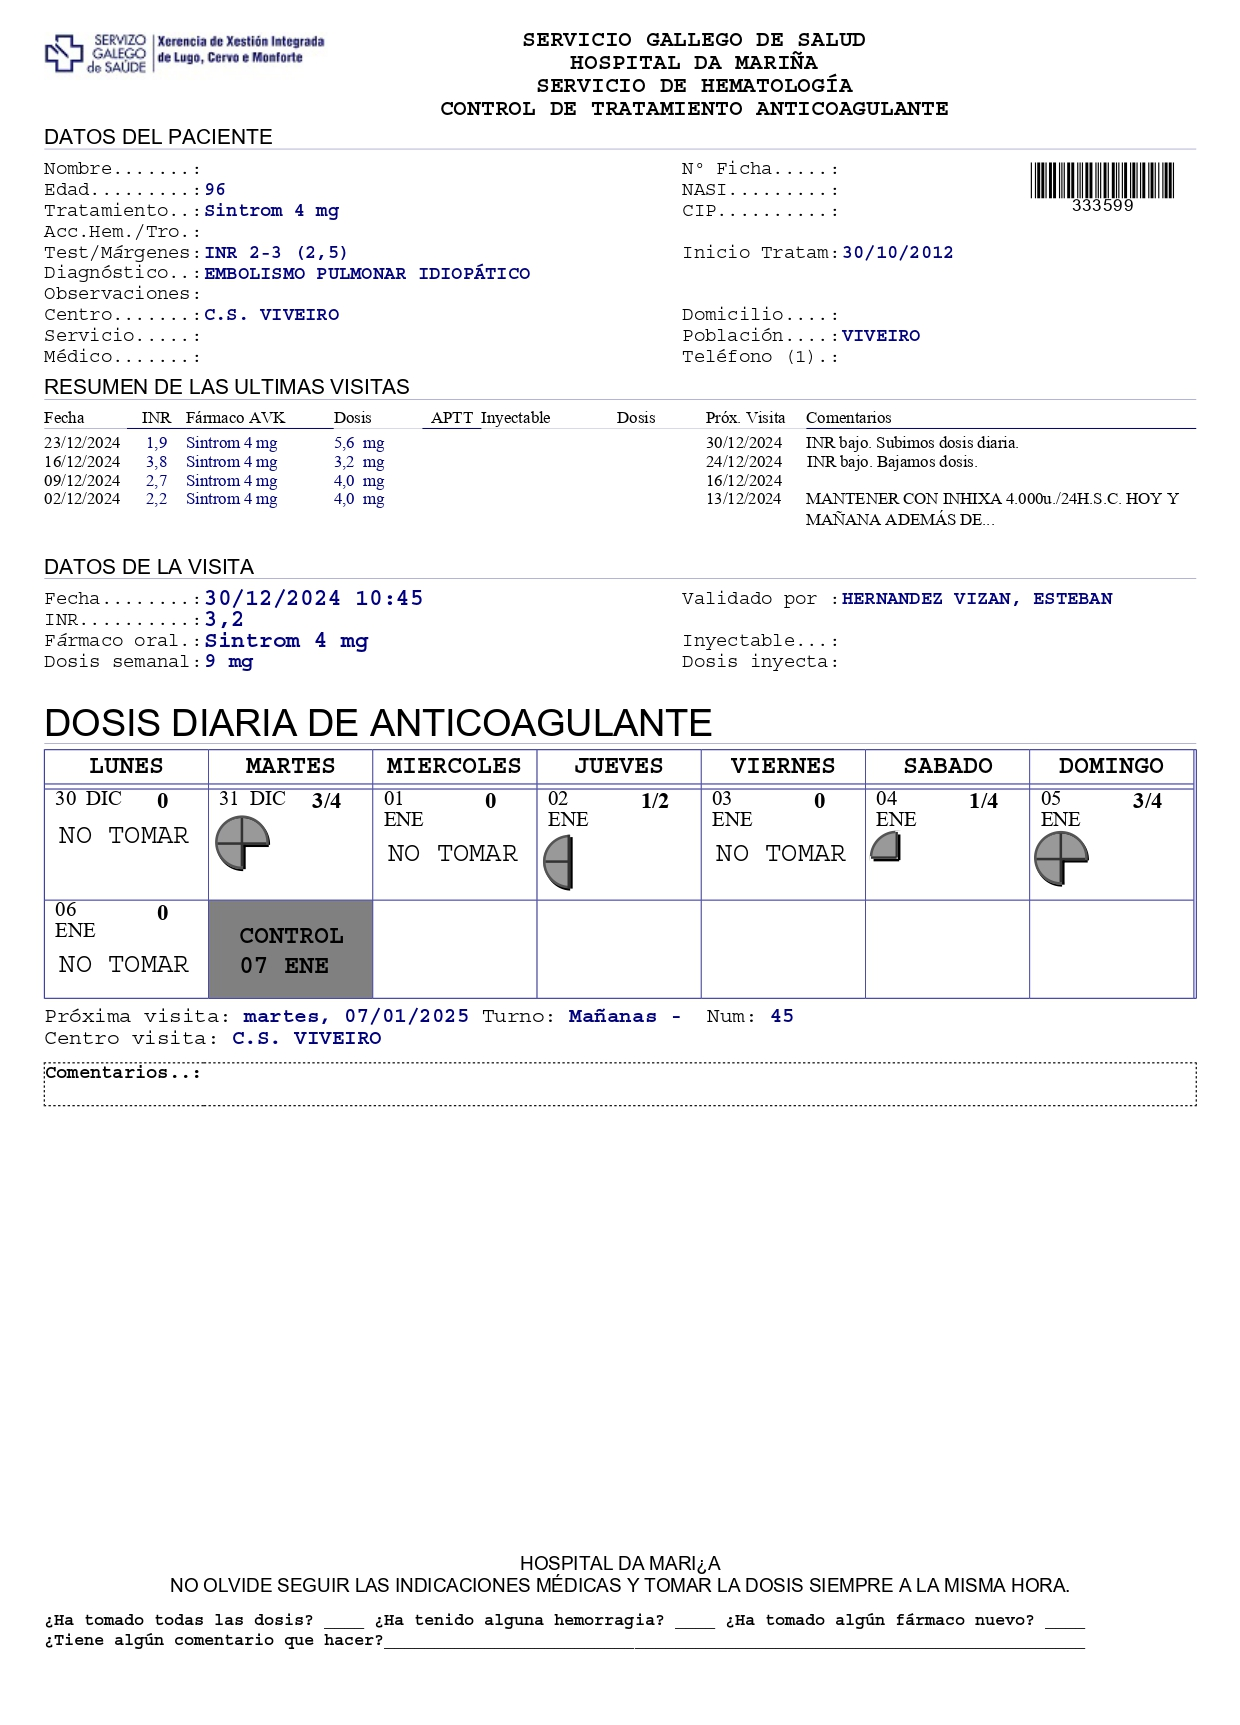
\includegraphics[width=0.7\textwidth]{imaxes/Introducion/IMAXE_SINTROM.jpg}
\caption{Exemplo de folla de tratamento}
\label{fig:follasintrom}
\end{figure}

\section{Motivación}

Este proxecto nace coa premisa de achegar seguridade ao tratamento e maior tranquilidade tanto aos pacientes como aos seus familiares e coidadores. Como se expuxo na sección anterior, no sistema actual, moitos pacientes viven coa constante preocupación de perder ou estragar a folla de tratamento. Ademais deben interpretar a pauta diaria a partir dunha táboa que pode resultar complexa e difícil de ler debido ao reducido tamaño de letra. Ao mesmo tempo, o proxecto busca aliviar os familiares ou coidadores, que adoitan vivir coa incerteza de non saber se a toma foi realizada correctamente.

A motivación principal deste proxecto é aproveitar as posibilidades que nos ofrecen os dispositivos móbiles para simplificar e reducir estes riscos ao mínimo. Para iso, proponse unha ferramenta \textbf{sinxela e intuitiva}, accesible para calquera persoa usuaria. A aplicación pretende dixitalizar a información do tratamento a partir dunha simple fotografía da folla de prescrición, permitindo extraer automaticamente toda a información necesaria e xerar recordatorios diarios para o paciente.

Ademais, incorpórase un sistema de confirmación das tomas. O paciente pode marcar na aplicación cando realiza a toma da dose que lle corresponde e, no caso de que esta non sexa rexistrada nun intervalo de tempo, o sistema envía unha notificación a un familiar ou coidador para que poida comprobar a situación e actuar no caso de que sexa necesario.

Deste modo, a aplicación busca transformar un proceso actualmente manual e dependente do papel nun sistema dixital e accesible que mellore a seguridade do paciente e facilite o seguimento do tratamento anticoagulante no día a día.

\section{Obxectivos}

O obxectivo principal deste proxecto é desenvolver unha aplicación móbil multiplataforma que facilite a xestión diaria do tratamento con Sintrom. Para logralo, establécense os seguintes obxectivos:
\begin{itemize}
    \item\textbf{ Eliminar a dependencia do papel:} Ao dixitalizar o informe, a información estará sempre dispoñible no móbil, evitando desprazamentos ao centro médico no caso de perda ou estragamento do documento orixinal.
    \item \textbf{Automatizar a entrada de datos mediante técnicas de procesado de imaxe:} Substituír a carga manual de información por un sistema que lea a imaxe da folla médica, reducindo os posibles erros ao copiar as doses.
    \item \textbf{Mellorar a seguridade nas tomas:} Reducir o risco de esquecementos mediante recordatorios programados e un sistema de avisos automáticos aos coidadores.
    \item \textbf{Facilitar o control a pacientes e coidadores: } Proporcionar un seguimento detallado das tomas e ofrecer un rexistro visual e sinxelo sobre a evolución histórica dos valores de \gls{inr} e da dose.
    \item \textbf{Garantir a privacidade dos datos:} Protexer a información médica evitando a súa persistencia nos servidores da aplicación, almacenando de forma segura os datos sensibles no dispositivo e cifrando a nivel de aplicación as mensaxes intercambiadas entre os dispositivos vinculados.
\end{itemize}

\section{Estudo de mercado}
Para avaliar a viabilidade deste proxecto, realizouse unha análise das solucións dispoñibles actualmente para o seguimento do tratamento de anticoagulante oral. A análise realizada mostra que o mercado se divide en dúas grandes categorías, aplicacións xenéricas de medicación e aplicacións específicas para Simtrom.


\subsection{Aplicacións xenéricas}
\label{subsec:aplicacións_xenericas}
Nesta categoría inclúense ferramentas que permiten a xestión xeral da medicación, permitindo crear recordatorios e rexistrar diferentes fármacos. 

Algunhas das app máis populares desta categoría son, por exemplo, \textit{Medisafe} \cite{AppMedisafe} ou \textit{MyTherapy} \cite{AppMyTherapy}. As capturas de ambas aplicacións recóllense no Apéndice~\ref{app:capturas-estudo-mercado}. Malia ser aplicacións bastante completas para o control de medicación xeral, non están adaptadas ás características específicas do tratamento anticoagulante. Algunhas das principais limitacións atopadas nestas solucións son:
\begin{itemize}
    \item \textbf{Xestión de pautas variables:} Estas aplicacións están deseñadas só para tratamentos recorrentes ou con doses fixas (ex. unha pastilla cada 8 horas, media pastilla cada 3 horas, unha pastilla diaria...). Se quixésemos empregar este tipo de apps para levar o control do tratamento de Sintrom teríamos que configurar, por exemplo, para unha folla cunha pauta de 7 días cunha dose cambiante diariamente, sete alarmas distintas con doses diferentes, o que induce ao erro.
    \item \textbf{Carga manual de datos:}  O usuario debe escribir cada medicamento e dose. Para unha persoa de avanzada idade isto resulta complexo e pode inducir a erros, creando unha gran barreira de uso da app.
\end{itemize}

\subsection{Aplicacións especializadas}
Existen algunhas solucións deseñadas especificamente para este tratamento como por exemplo:
\begin{itemize}
    \item \textbf{AnticoagulApp} \cite{AppAnticoagulApp}: Esta é unha aplicación lanzada pola \textit{Sociedade Española de Cardioloxía} que permite rexistrar o \gls{inr}, as doses e ofrece consellos de saúde. Se ben mellora as alternativas xenéricas ao adaptarse ás doses variables, mantén a barreira principal, xa que require que o usuario rexistre as doses manualmente. Non ten capacidade de interpretar documentos físicos, obrigando ao paciente a ler e transcribir a folla do médico. A súa interface pode consultarse na Figura~\ref{fig:AppAnticoagulApp} do Apéndice~\ref{app:capturas-estudo-mercado}. \footnote{Durante o período de redacción da memoria deste traballo esta aplicación non está dispoñible xa que se atopa en proceso de actualizacións.}
    \item \textbf{INR Diary} \cite{AppINRDiary}:  Aínda que permite un rexistro detallado do \gls{inr} e das doses tomadas, a entrada de datos segue a ser completamente manual. Ademais esta aplicación é de pago, o que supón unha barreira económica engadida que limita a súa accesibilidade para gran parte dos pacientes.  A súa interface móstrase na Figura~\ref{fig:AppINRDiary} do Apéndice~\ref{app:capturas-estudo-mercado}.
\end{itemize}

\FloatBarrier

\begin{table}[hp!]
  \centering
  \caption{Comparativa de funcionalidades das aplicacións existentes e da nosa solución}
  \rowcolors{2}{white}{udcgray!25}
  \resizebox{\textwidth}{!}{
  \begin{tabular}{c|c|c|c|c}
  \rowcolor{udcpink!25}
  \textbf{Funcionalidade} & \textbf{App Xenérica} & \textbf{AnticoagulApp} & \textbf{INR Diary} & \textbf{SintromApp} \\\hline
  \textit{Recordatorios Sonoros} & Si & Si & Si & Si \\
  \textit{Histórico INR} & Non & Si & Si & Si \\
  \textit{Entrada por técnicas de procesado de imaxe} & Non & Non & Non & Si \\
  \textit{Aviso a coidadores} & Algunhas & Non & Non & Si \\
  \textit{Dose diaria variable} & Manual & Manual & Manual & Automática \\
  \end{tabular}
  }
  \label{tab:comparativa}
\end{table}


Como se pode observar na Táboa \ref{tab:comparativa}, as solucións existentes presentan limitacións importantes no contexto específico do tratamento con Sintrom. Ningunha das aplicacións analizadas permite extraer automaticamente a información a partir dunha folla de prescrición médica, delegando a responsabilidade da carga de datos no paciente.

Para dar resposta a estas limitacións, a nosa proposta introduce unha solución centrada na automatización e na adaptación ás necesidades reais dos pacientes anticoagulados. Concretamente, a ferramenta \textbf{desmarcarase} das alternativas actuais baseándose nos seguintes piares:

\begin{itemize}
    \item \textbf{Automatización mediante procesado de imaxe:} A aplicación \textbf{é capaz} de ler e interpretar a folla do SERGAS mediante a cámara do dispositivo, eliminando por completo a necesidade de que o paciente teña que teclear as súas doses.
    \item \textbf{Adaptación nativa a pautas variables:} A lóxica do sistema \textbf{está deseñada} especificamente para o Sintrom, xestionando de forma autónoma as doses cambiantes de cada día sen requirir múltiples configuracións manuais.
    \item \textbf{Rede de seguridade familiar:} \textbf{Intégrase} un sistema de notificacións que avisará automaticamente aos coidadores ou familiares en caso de que o paciente se esqueza da súa toma diaria.
    \item \textbf{Foco na fenda dixital:} Para romper as barreiras de adopción tecnolóxica, a interface \textbf{conta} cun ``modo sinxelo'' pensado especificamente para persoas de avanzada idade.
\end{itemize}

Con este conxunto de funcionalidades, o proxecto \textbf{busca} cubrir un oco baleiro no mercado, ofrecendo unha ferramenta que non só rexistre datos, senón que reduza a carga cognitiva do usuario e achegue unha tranquilidade real tanto ao paciente como á súa contorna.

\section{Estrutura do documento}

A memoria organízase nos seguintes capítulos:

\begin{itemize}
\item \textbf{Capítulo~\ref{chap:introducion} -- Introdución:} presenta o contexto, a motivación, os obxectivos e o estudo de mercado.

    \item \textbf{Capítulo~\ref{chap:metodoloxia} -- Metodoloxía:} describe o enfoque iterativo, Kanban e a xestión do código.

    \item \textbf{Capítulo~\ref{chap:tecnoloxias} -- Tecnoloxías empregadas:} recolle as principais ferramentas e servizos utilizados.

    \item \textbf{Capítulo~\ref{chap:Analise} -- Análise:} define o alcance, os requisitos e os casos de uso.

    \item \textbf{Capítulo~\ref{chap:planificacion} -- Planificación e seguimento:} presenta a dedicación, os custos e as desviacións.

    \item \textbf{Capítulo~\ref{chap:procesamento-follas} -- Procesamento automático:} compara as alternativas e xustifica a solución seleccionada.

    \item \textbf{Capítulo~\ref{chap:deseño} -- Deseño:} describe a arquitectura, os datos, os fluxos e a interface.

    \item \textbf{Capítulo~\ref{chap:implem} -- Implementación:} explica a construción da API e do cliente móbil.

    \item \textbf{Capítulo~\ref{chap:probas} -- Probas:} presenta as comprobacións realizadas e a cobertura obtida.

    \item \textbf{Capítulo~\ref{chap:conclusions} -- Conclusións:} valora o cumprimento dos obxectivos e propón posibles melloras futuras.
\end{itemize}
 \chapter{Metodoloxía}
\label{chap:metodoloxia}

O proxecto desenvolveuse mediante un enfoque \textbf{incremental e iterativo}, empregando un taboleiro \textbf{Kanban} para organizar as tarefas e realizar o seu seguimento. Esta forma de traballo permitiu avanzar por etapas, comprobar os resultados de cada unha e adaptar o desenvolvemento ás necesidades que foron aparecendo.

Optouse por un fluxo continuo de traballo, no que as tarefas se priorizaron segundo a súa importancia para o funcionamento principal do sistema, as dependencias existentes, a dificultade e a incerteza técnica e a proximidade dos fitos establecidos.

\section{Enfoque incremental e iterativo}

O desenvolvemento incremental consiste en construír o sistema mediante etapas sucesivas que amplían progresivamente as súas capacidades. Cada incremento parte dos resultados obtidos nos anteriores e incorpora novas funcionalidades ou melloras.

O carácter iterativo permite revisar e modificar solucións xa desenvolvidas cando aparecen novos datos ou necesidades. Isto foi especialmente importante neste proxecto, xa que a estrutura das follas de tratamento, os resultados das técnicas de extracción e os requisitos da aplicación móbil fóronse coñecendo con maior precisión durante o desenvolvemento.

En lugar de desenvolver a aplicación completa desde o principio, o traballo dividiuse en varios pasos. Primeiro estudouse se era posible extraer os datos automaticamente dos documentos, despois desenvolveuse unha API capaz de procesar as follas de tratamento e, finalmente, creouse a aplicación móbil que consume esa API e permite utilizar os resultados.

Esta forma de traballo evitou desenvolver a aplicación móbil arredor dunha tecnoloxía de extracción que podía non ofrecer resultados suficientemente fiables. Ademais, permitiu comprobar o funcionamento de cada compoñente antes de realizar a integración completa do sistema.

Os incrementos concretos nos que se dividiu o desenvolvemento e o seu seguimento temporal descríbense no capítulo (\ref{chap:planificacion}).

\section{Aplicación de Kanban}

Kanban é un método de xestión visual que permite representar as tarefas do proxecto segundo o seu estado. Cada tarefa móvese entre distintas columnas a medida que avanza o seu desenvolvemento, o que facilita coñecer o traballo pendente, identificar as actividades que se están realizando e comprobar as que xa foron completadas.  Para aplicar Kanban no proxecto empregouse un taboleiro de GitHub Projects con catro estados:
\begin{itemize}
    \item \textbf{Para máis adiante:} ideas, melloras ou tarefas que se consideraban útiles, pero que non formaban parte do traballo inmediato.
    \item \textbf{Por facer:} tarefas xa definidas, revisadas e priorizadas que estaban preparadas para comezar.
    \item \textbf{En curso:} tarefas nas que se estaba traballando ou que permanecían pendentes dalgunha comprobación.
    \item \textbf{Feito:} tarefas completadas e comprobadas.
\end{itemize}

Na Figura~\ref{fig:taboleiro-kanban} móstrase o estado do taboleiro
Kanban nun momento do desenvolvemento, coas tarefas
distribuídas segundo o seu estado.

O movemento das tarefas entre as columnas non se realizaba automaticamente. As tarefas situadas en \textit{Para máis adiante} revisábanse periodicamente e trasladábanse a \textit{Por facer} cando pasaban a formar parte dos obxectivos próximos do proxecto. Nese momento comprobábase tamén que estivesen suficientemente definidas e que a prioridade asignada seguise sendo adecuada.

Para iniciar unha nova tarefa seleccionábase unha das actividades da columna \textit{Por facer}, atendendo en primeiro lugar á prioridade que tiña asignada. Cando varias tarefas compartían o mesmo nivel, tíñanse en conta as dependencias con outras actividades, a incerteza técnica e a existencia de posibles bloqueos. Antes de movela a \textit{En curso}, comprobábase tamén que non se superase o límite de traballo establecido.

Unha vez iniciado o traballo, a tarefa permanecía na columna \textit{En curso} durante a súa realización e comprobación. Se para completala era necesario realizar modificacións adicionais, probas ou integracións con outros compoñentes, continuaba nesta columna ata que se resolvesen.

Unha tarefa só se trasladaba a \textit{Feito} despois de cumprir os criterios de aceptación, realizar as comprobacións necesarias e integrar o resultado no proxecto. Deste xeito, a existencia dunha implementación parcial non era suficiente para considerar unha tarefa rematada.

O movemento seguido polas tarefas entre as distintas columnas represéntase na Figura~\ref{fig:diagrama-kanban}.
\FloatBarrier

 \begin{figure}
     \centering
     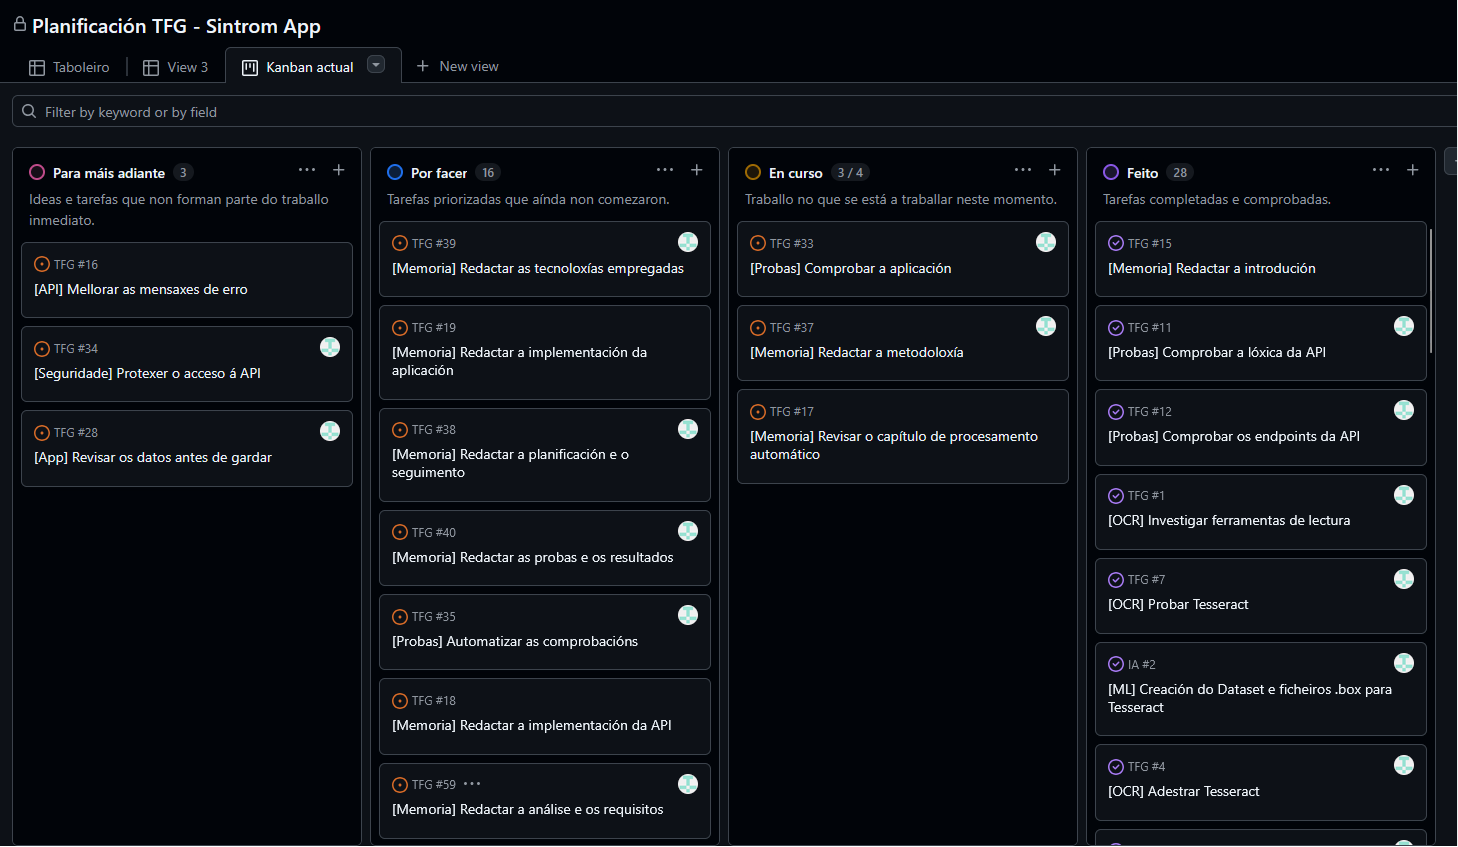
\includegraphics[width=1\linewidth]{imaxes/02-Metodoloxía/taboleiro-kanban.png}
     \caption{Estado do taboleiro Kanban o 20 de Xullo de 2026.}
     \label{fig:taboleiro-kanban}
 \end{figure}
 
\begin{figure}[h!]
    \centering
    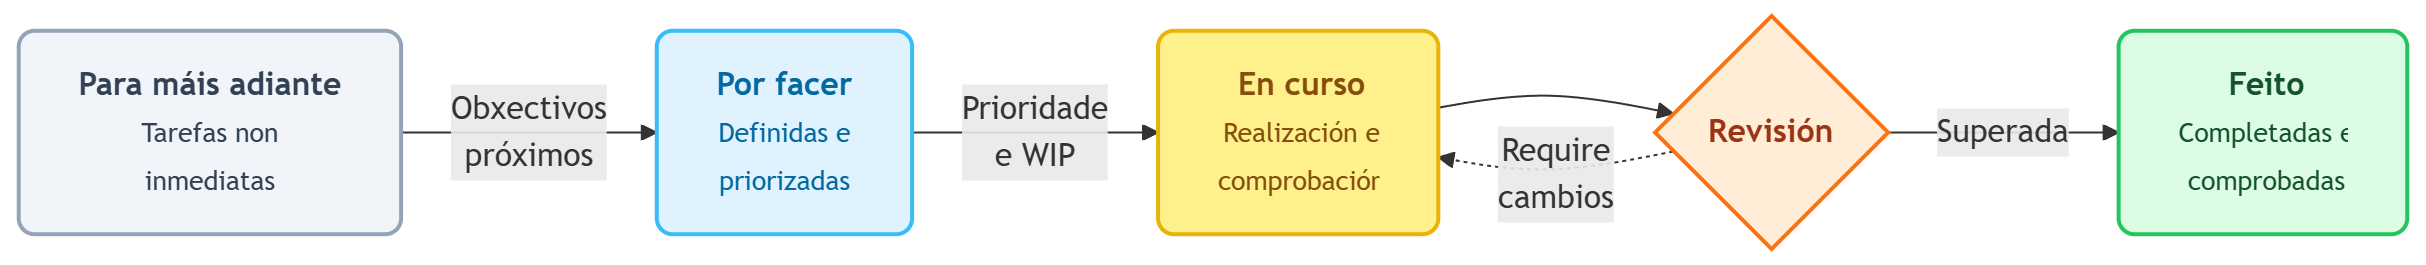
\includegraphics[width=1\linewidth]{imaxes/02-Metodoloxía/diagrama-kanban.png}
    \caption{Diagrama do fluxo de tarefas no taboleiro Kanban.}
    \label{fig:diagrama-kanban}
\end{figure}

\subsection{Límite de traballo en curso}

Estableceuse un límite de traballo en curso, ou límite WIP (\textit{Work In Progress}), de \textbf{catro tarefas}. O seu obxectivo foi favorecer a finalización das tarefas iniciadas antes de comezar outras novas.

Escolleuse este valor porque permitía manter activas tarefas de distintas áreas do proxecto sen acumular un número excesivo de actividades abertas. No cómputo do límite incluíanse tamén as tarefas pendentes de revisión, validación ou
desbloqueo, polo que non implicaba que se desenvolvesen catro tarefas simultaneamente.

Cando se alcanzaba o límite, priorizábase a finalización, integración ou desbloqueo das tarefas existentes antes de iniciar outras novas.


\subsection{Organización e priorización das tarefas}

Cada tarefa do taboleiro representouse mediante unha \textit{issue} de GitHub. Nela recollíanse a descrición do traballo, os criterios de aceptación, a prioridade, as etiquetas e, cando correspondía, as relacións con outras tarefas ou \textit{pull requests}.

Na Figura~\ref{fig:exemplo-tarefa} preséntase unha das tarefas do proxecto, na que se poden observar algúns destes elementos.

\begin{figure}[h!]
    \centering
    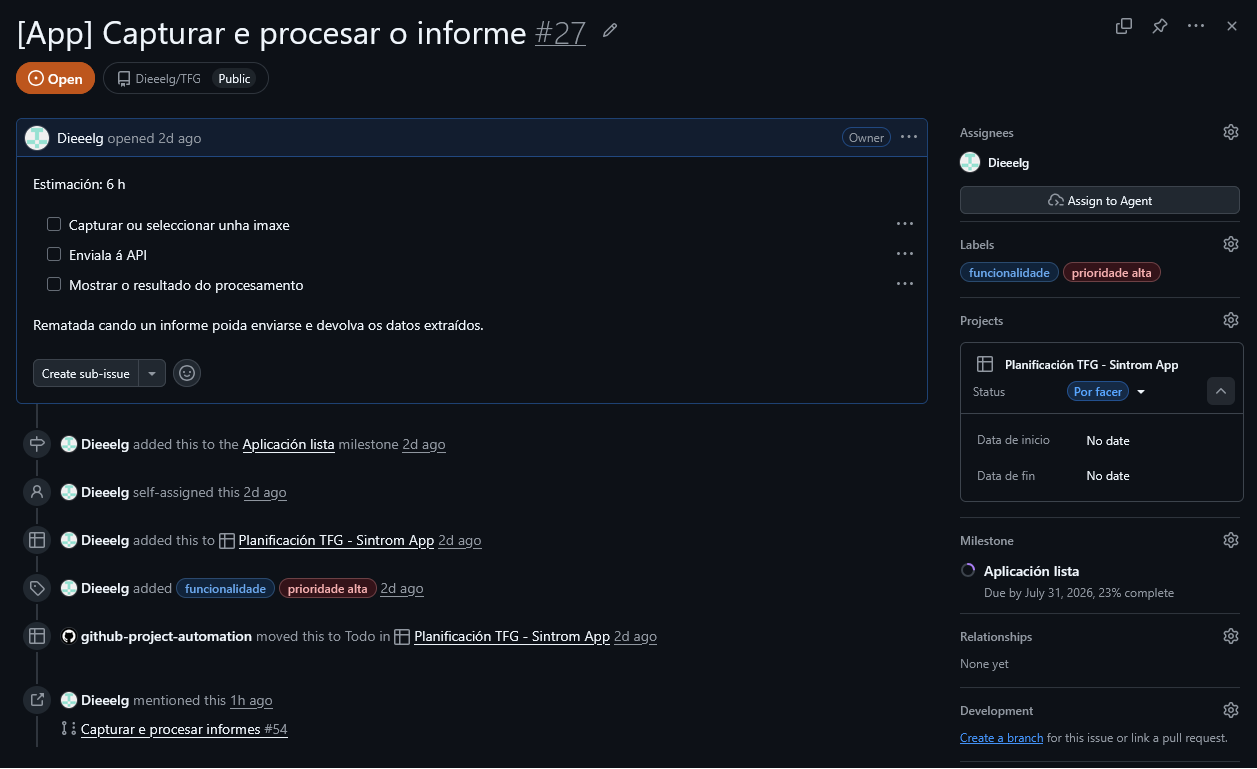
\includegraphics[width=1\linewidth]{imaxes/02-Metodoloxía/exemploTarefa.png}
    \caption{Exemplo dunha tarefa do proxecto.}
    \label{fig:exemplo-tarefa}
\end{figure}
\FloatBarrier

Para representar a prioridade das tarefas empregáronse tres etiquetas:

\begin{itemize}
    \item \textbf{Prioridade alta}: tarefas que debían realizarse canto antes, especialmente cando bloqueaban o fluxo principal ou outras actividades.
    \item \textbf{Prioridade media}: tarefas importantes, pero que non impedían continuar co desenvolvemento.
    \item \textbf{Prioridade baixa}: tarefas que podían pospoñerse ata completar as funcionalidades principais.
\end{itemize}

As tarefas priorizáronse atendendo principalmente á súa importancia para completar o fluxo principal, ás dependencias con outras tarefas, á dificultade e á incerteza técnica, á proximidade do fito ao que pertencían e á existencia de bloqueos que impedisen avanzar noutras funcionalidades.

Deste xeito, as funcionalidades necesarias para procesar unha folla de tratamento, gardar os datos, consultar a pauta e confirmar unha toma recibiron unha prioridade superior ás melloras visuais. Do mesmo xeito, unha corrección que bloqueaba varias tarefas tiña prioridade sobre unha funcionalidade independente que podía incorporarse máis adiante.

O taboleiro revisouse periodicamente e ao finalizar cada incremento. Durante estas revisións actualizáronse os estados e as prioridades das tarefas, e identificáronse posibles bloqueos ou actividades que permanecían demasiado tempo en curso.

Cando unha tarefa resultaba demasiado extensa ou combinaba cambios non relacionados, dividíase en tarefas máis pequenas para facilitar a súa estimación, desenvolvemento e comprobación.

\section{Aplicación de GitFlow ao control de versións}
\label{sec:gitflow}

Para xestionar as distintas versións do código empregáronse Git e GitHub xunto cunha adaptación simplificada de GitFlow. Este modelo permite separar o código estable do código en desenvolvemento e realizar cada cambio nunha rama independente antes de integralo~\cite{DriessenGitFlow}.

No proxecto utilizáronse os seguintes tipos de ramas:
\begin{itemize}
    \item \textit{master}: mantívose como referencia estable do proxecto.
    \item \textit{develop}: empregouse como rama de integración das funcionalidades xa comprobadas.
    \item \textit{feature/nome-da-tarefa}: utilizouse para desenvolver novas funcionalidades. Algúns exemplos son \textit{feature/calendario},  \textit{feature/confirmar-tomas} ou \textit{feature/vincular-coidador}
    \item \textit{fix/nome-do-problema}: empregouse para correccións concretas, como \textit{fix/configuracion-local} e \textit{fix/datos-centros}.
\end{itemize}

\begin{figure}[h!]
    \centering
    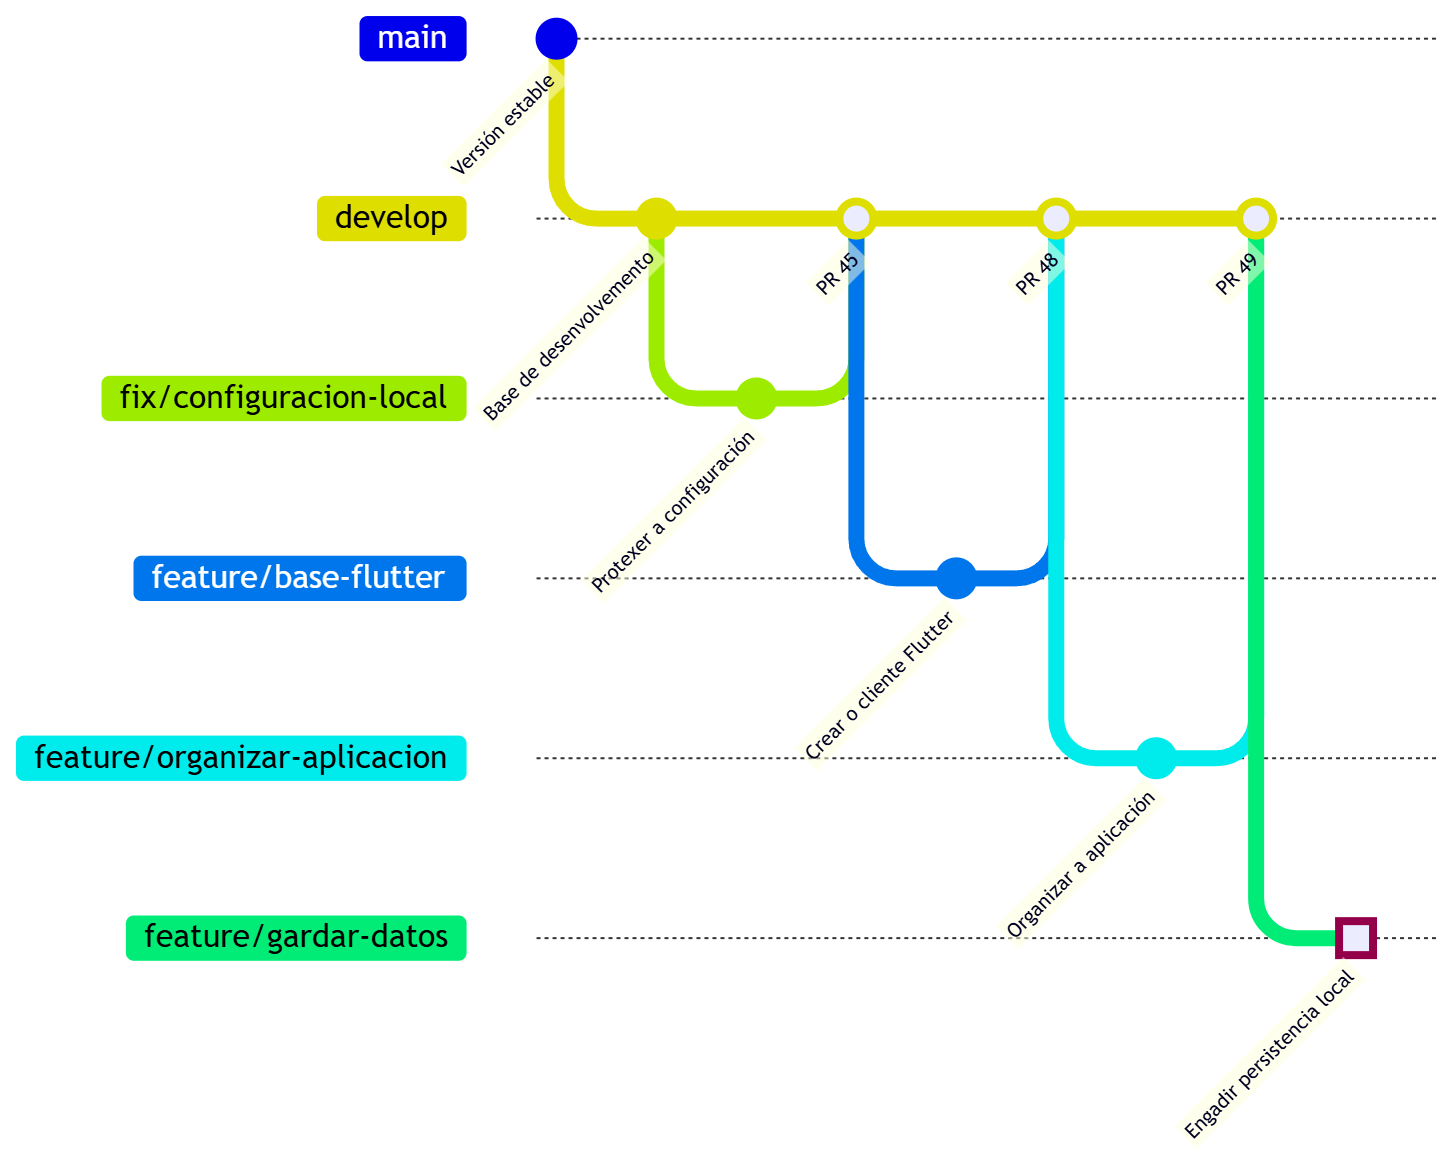
\includegraphics[width=0.7\linewidth]{imaxes/02-Metodoloxía/diagrama-gitflow.png}
    \caption{Adaptación de GitFlow empregada no proxecto.}
    \label{fig:diagrama-gitflow}
\end{figure}

Para ilustrar este fluxo de traballo, a Figura~\ref{fig:diagrama-gitflow} mostra unha representación visual dalgunhas das ramas empregadas no proxecto. No grafo pódese observar a rama principal (\textit{main}) e a base de desenvolvemento (\textit{develop}), así como exemplos reais do historial. As ramas resoltas, como \textit{fix/configuracion-local} ou \textit{feature/base-flutter}, parten de \textit{develop} e intégranse de novo a través das súas respectivas \textit{pull requests} (como as PR 45, PR 48 e PR 49). Pola contra, o traballo en curso, como a rama \textit{feature/gardar-datos}, mantense illado ata a súa finalización.


As ramas de funcionalidades e correccións creábanse a partir de \textit{develop}.  O código nunca se modificou directamente sobre as ramas principais, garantindo así o illamento de cada tarefa. Durante o desenvolvemento, os cambios rexistráronse aplicando a convención de \textit{commits} semánticos (empregando prefixos como \textit{feat:}, \textit{fix:}, \textit{refactor:} ou \textit{chore:}). Isto permitiu manter un historial lexible e descritivo que indica claramente o propósito de cada modificación.

Unha vez rematada unha tarefa, a rama correspondente publicábase no repositorio remoto e abríase unha \textit{pull request} cara a rama \textit{develop}. Este mecanismo empregouse aínda que o proxecto fose desenvolvido por unha única persoa. Neste contexto non proporcionaban unha revisión independente, pero si ofrecían un punto de control antes de modificar \textit{develop}. Ademais, permitían consultar a descrición do cambio, os commits incluídos, os ficheiros modificados e a relación coa tarefa correspondente.

Na Figura~\ref{fig:exemplo-pull-request} móstrase un exemplo deste proceso, correspondente á integración mediante \textit{pull request} dunha das tarefas de desenvolvemento.

\begin{figure}[h!]
    \centering
    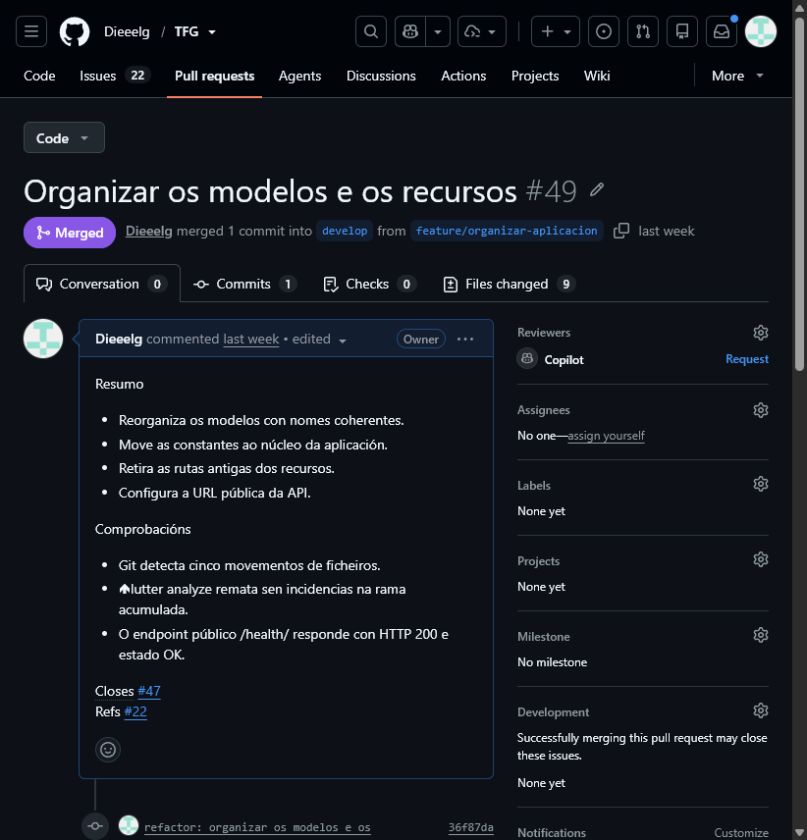
\includegraphics[width=0.7\linewidth]{imaxes/02-Metodoloxía/exemplo-pull-request.png}
    \caption{Integración dunha rama de funcionalidade en \textit{develop} mediante unha \textit{pull request}.}
    \label{fig:exemplo-pull-request}
\end{figure}



A principal diferenza desta adaptación con respecto ao modelo orixinal foi a omisión das ramas de \textit{release} e \textit{hotfix}. Dado que o proxecto non requiría manter simultaneamente varias versións publicadas en produción, esta simplificación permitiu conservar as vantaxes principais do illamento de código sen introducir unha complexidade innecesaria no fluxo de traballo.

\section{Xustificación da metodoloxía}

A combinación dun desenvolvemento incremental e iterativo cun taboleiro Kanban resultou axeitada para as características e necesidades do proxecto. Durante as primeiras etapas existía unha elevada incerteza sobre a viabilidade da extracción automática dos datos e sobre a tecnoloxía máis axeitada para realizala. Por este motivo, resultaba difícil establecer desde o inicio unha planificación pechada ou estimar con precisión a duración das tarefas de investigación e experimentación.

O enfoque incremental permitiu avanzar por etapas e reducir progresivamente esta incerteza. Primeiro estudouse a viabilidade da extracción automática, despois seleccionouse unha tecnoloxía e desenvolveuse unha primeira versión funcional da API e, finalmente, construíuse a aplicación móbil. Cada incremento proporcionou un resultado comprobable que serviu como base para continuar co desenvolvemento.

O carácter iterativo permitiu revisar solucións xa desenvolvidas cando se obtiveron novos resultados. As decisións relacionadas coa extracción dos datos, a organización da API e o funcionamento da aplicación fóronse modificando e refinando a medida que se coñecían mellor a estrutura das follas de tratamento e as necesidades do sistema.

Non se aplicou Scrum de maneira estrita porque a organización do traballo en sprints de duración fixa non se considerou a opción máis axeitada para unhas tarefas cunha duración e uns resultados difíciles de prever. En cambio, Kanban permitiu manter un fluxo continuo, modificar as prioridades segundo os avances realizados e incorporar novas tarefas cando se detectaban necesidades ou problemas.

O taboleiro proporcionou unha representación visual do estado do proxecto, diferenciando as tarefas pendentes, as que se atopaban en desenvolvemento e as que xa foran comprobadas. O límite de traballo en curso favoreceu a finalización das tarefas iniciadas antes de abrir novas liñas de traballo e permitiu identificar aquelas que permanecían pendentes de revisión ou validación.

No relativo á xestión do código, o uso de GitFlow axudou a manter o traballo moito máis organizado. O feito de programar cada tarefa nunha rama separada e usar \textit{pull requests} obrigou a facer unha revisión persoal de cada cambio antes de integralos no código principal. Ademais, o emprego de \textit{commits} semánticos permitiu crear un historial moito máis claro, onde é moi doado entender os pasos que se foron dando.

Como principal limitación, ao tratarse dun proxecto individual non se contou cunha revisión independente continua do traballo realizado. Para reducir este risco combinouse a auto-revisión nas \textit{pull requests} co uso de criterios de aceptación, listas de comprobación e comprobacións técnicas e funcionais antes de integrar os cambios e considerar completadas as tarefas.
\chapter{Tecnoloxías empregadas}
\label{chap:tecnoloxias}

Neste capítulo preséntanse as tecnoloxías empregadas tanto no desenvolvemento da solución como nas probas realizadas durante o estudo da extracción automática das follas de tratamento. A solución está formada por un cliente móbil e por unha \gls{api} que centraliza o procesamento das follas de tratamento e a comunicación cos servizos externos.

%No relativo á extracción automática de información, neste capítulo descríbese unicamente a tecnoloxía finalmente integrada na solución, Azure AI Document Intelligence. As alternativas avaliadas durante o proxecto e os seus resultados experimentais forman parte do Capítulo~\ref{chap:procesamento-follas}.

%A selección realizouse atendendo a cinco criterios sinxelos: adecuación ás necesidades do proxecto, facilidade de integración, dispoñibilidade de documentación, posibilidade de reutilizar código e reproducibilidade do contorno. Tamén se valorou que as ferramentas tivesen unha comunidade activa e que puidesen empregarse cun custo asumible nun traballo académico.

\section{Linguaxes de programación}

\subsection{Dart}
O cliente móbil para Android desenvolveuse empregando Dart~\cite{DartDocs} (\textit{versión 3.9.2}). Trátase dunha linguaxe orientada a obxectos e deseñada especificamente para o desenvolvemento de aplicacións con interfaces de usuario rápidas e multiplataforma.

A súa elección para este proxecto vén motivada pola súa estreita integración co framework de Flutter. Esta combinación permite empregar unha mesma linguaxe para definir tanto o deseño visual das pantallas como a lóxica interna da aplicación. Deste xeito, simplifícase a estrutura do cliente e evítase cambiar de linguaxe entre a parte visual e o seu comportamento, o que axiliza notablemente o proceso de desenvolvemento.

Outro aspecto que facilitou a súa elección foi a familiaridade da súa sintaxe. Dart comparte conceptos con outras linguaxes orientadas a obxectos, como Java, polo que os coñecementos previos nesta tecnoloxía facilitaron a adaptación ao novo contorno de desenvolvemento.

No contexto do proxecto, Dart empregouse para construír as pantallas, representar os modelos de datos, xestionar o estado da sesión e as preferencias do usuario, e realizar as comunicacións asíncronas coa \gls{api}.


\subsection{Python}
A \gls{api} foi implementada con Python ~\cite{PythonDocs} (\textit{versión 3.11.3}). Python é unha linguaxe de programación de alto nivel e propósito xeral, caracterizada por ofrecer unha sintaxe sinxela e lexible. Estas características permiten expresar a lóxica da aplicación de forma clara e favorecen a organización e o mantemento do código.

A súa elección para este proxecto debeuse principalmente á variedade de bibliotecas dispoñibles para o desenvolvemento de servizos web, o procesamento de imaxes e a integración con plataformas externas. Isto permitiu implementar nun mesmo contorno as diferentes tarefas realizadas pola parte servidora, evitando incorporar tecnoloxías adicionais e reducindo a complexidade da solución.

No contexto do proxecto, Python empregouse para implementar a lóxica da \gls{api}, recibir e validar os datos enviados pola aplicación móbil, coordinar as operacións necesarias na parte servidora e devolver os resultados nun formato que puidese ser consumido polo cliente.

\section{Marcos de desenvolvemento }

\subsection{Flutter}
Flutter~\cite{FlutterArchitecture} (\textit{versión 3.35.5}) é o marco de traballo empregado para construír a aplicación móbil.  A súa forma de traballar baséase no uso de \textit{widgets}, pezas visuais reutilizables que permiten construír as pantallas da interface de forma sinxela e estruturada. Este marco incorpora o seu propio motor de renderizado, os compoñentes de interface e as ferramentas necesarias para a construción da aplicación.  Aínda que Flutter é unha tecnoloxía deseñada para crear aplicacións en varios sistemas simultaneamente, o alcance deste proxecto limítase a Android, polo que a solución foi desenvolvida e probada exclusivamente para esta plataforma.

No relativo ao deseño, a aplicación emprega as directrices de Material 3 ~\cite{MaterialDesign3} como sistema visual principal. Isto permite manter unha aparencia coherente e moderna en toda a aplicación usando compoñentes xa estandarizados. Ademais, durante o desenvolvemento, a característica de recarga en quente (\textit{hot reload}) resultou de gran axuda, xa que permitiu visualizar os cambios na interface de maneira case instantánea, axilizando moito o traballo.

Por último, a elección de Flutter tamén se xustifica pola súa facilidade para acceder ás funcións nativas do teléfono mediante complementos \textit{plugins})~\cite{FlutterPlugins}. No caso desta aplicación, foron imprescindibles para acceder ao almacenamento seguro do dispositivo, xestionar a cámara para a lectura de códigos \gls{qr} e recibir notificacións. En resumo, a súa perfecta integración con Dart, a comodidade para crear interfaces e a dispoñibilidade de paquetes listos para usar convertérono na opción ideal para o proxecto.

\subsection{FastAPI}

FastAPI~\cite{FastAPIFeatures} (\textit{versión 0.119.1}) é o marco de traballo web sobre o que se construíu a \gls{api} do proxecto. Esta ferramenta permite declarar as operacións \gls{http} empregando directamente funcións e anotacións de tipo (\textit{type annotations}) de Python. A partir destas declaracións, o marco encárgase de validar os datos automaticamente e de xerar unha especificación OpenAPI con interfaces de documentación interactivas.

No contexto do proxecto, FastAPI utilízase como a ponte de comunicación entre a aplicación móbil e os distintos servizos externos. A \gls{api} permite recibir as follas de tratamento, coordinar o seu procesamento e devolver os resultados estruturados en formato \gls{json}. Ademais, proporciona un punto de acceso para comprobar o estado do servizo e enviar as actualizacións e avisos entre os dispositivos vinculados.

A escolla de FastAPI fronte a outros marcos populares de Python, como Django ou Flask, xustifícase polo seu enfoque moderno e orientado á creación de \glspl{api}. Para as necesidades deste proxecto, Django considerouse unha alternativa máis ampla do necesario, ao incorporar de serie funcionalidades como un ORM e outros compoñentes orientados ao desenvolvemento de aplicacións web completas~\cite{DjangoOverview}. Pola súa parte, Flask ofrece un núcleo máis reducido, pero determinadas funcionalidades adicionais deben incorporarse mediante extensións~\cite{FlaskExtensions}. FastAPI ofrece soporte asíncrono e integración directa con Pydantic, permitindo dispoñer de validación de datos e documentación automática da \gls{api}~\cite{FastAPIFeatures}.

\section{Tecnoloxías para o procesamento automático de documentos}
\label{sec:tecnoloxias-procesamento}

Durante o estudo da extracción automática das follas de tratamento empregáronse diferentes tecnoloxías de recoñecemento de texto, detección de obxectos, anotación de imaxes e procesamento documental. O procedemento seguido nas probas con cada unha delas descríbese no Capítulo~\ref{chap:procesamento-follas}.

\subsection{Google ML Kit}
\label{sec:tec-mlkit}

Google ML Kit é un conxunto de ferramentas de aprendizaxe automática orientado á incorporación de funcionalidades de visión artificial en aplicacións móbiles. Entre os seus módulos inclúese o recoñecemento de texto en imaxes, que permite identificar texto e obter información sobre a súa distribución na imaxe~\cite{GoogleMLKitTextRecognition}.

\subsection{Tesseract}
\label{sec:tec-tesseract}

Tesseract é un motor de recoñecemento óptico de caracteres de código aberto orientado á extracción de texto a partir de imaxes e documentos dixitalizados. Dispón de modelos para diferentes idiomas e permite tamén crear modelos adaptados a documentos concretos~\cite{TesseractOCR}.

\subsection{YOLO}
\label{sec:tec-yolo}

\gls{yolo} é unha familia de modelos de detección de obxectos baseada en redes neuronais. Permite localizar e clasificar elementos presentes nunha imaxe mediante caixas delimitadoras, polo que, a diferenza dun sistema de \gls{ocr}, está orientado á identificación de obxectos e non á extracción directa de texto~\cite{UltralyticsYOLO}.

\subsection{CVAT}
\label{sec:tec-cvat}

\gls{cvat} é unha ferramenta de anotación de imaxes orientada á preparación de conxuntos de datos para tarefas de visión artificial. Permite marcar manualmente rexións dunha imaxe e asignarlles as clases que posteriormente poden utilizarse para adestrar modelos de detección~\cite{CVATDocumentation}.

\subsection{Azure AI Document Intelligence}
\label{sec:tec-azure-di}
\label{sec:azure-document-intelligence}

Azure AI Document Intelligence é un servizo na nube de Microsoft orientado á extracción de información estruturada a partir de documentos. Permite identificar campos, táboas e outros elementos e ofrece tanto modelos preadestrados como modelos personalizados para documentos cunha estrutura específica~\cite{AzureDocumentIntelligence}.

Para a creación e xestión destes modelos empregouse Azure AI Document Intelligence Studio~\cite{AzureDocumentIntelligenceStudio}, a interface web proporcionada por Microsoft para traballar co servizo.

\section{Bibliotecas}

\subsection{Bibliotecas do cliente móbil}

As bibliotecas do cliente seleccionáronse para resolver necesidades concretas e evitar programar desde cero funcións que xa están consolidadas na comunidade:

\begin{description}
  \item[Provider 6.1.5+1] Emprégase para xestionar a información que se comparte entre as diferentes pantallas da aplicación. Deste xeito, calquera cambio nos datos actualiza a interface automaticamente~\cite{ProviderPackage}. A súa elección débese a que permite separar claramente o deseño visual da lóxica da aplicación, mantendo o código organizado e doado de manter.

  \item[HTTP 1.6.0] Utilízase para realizar as comunicacións coa \gls{api}, como o envío dos documentos escaneados e a recepción dos resultados~\cite{DartHttpPackage}. Escolleuse por ser unha solución robusta e un estándar dentro da comunidade para xestionar peticións asíncronas e comunicarse con servizos web.

  \item[Flutter Secure Storage 9.2.4] Permite gardar información sensible aproveitando os mecanismos de almacenamento protexido proporcionados por Android~\cite{FlutterSecureStorage}. No proxecto utilízase para conservar os identificadores da instalación, os datos das vinculacións e as claves criptográficas compartidas entre os dispositivos. Seleccionouse porque esta información non debe gardarse como texto simple na base de datos SQLite do dispositivo mobil nin nos ficheiros ordinarios da aplicación.
  
  \item[Cryptography 2.9.0] Proporciona os algoritmos necesarios para cifrar as mensaxes intercambiadas entre pacientes e supervisores~\cite{CryptographyPackage}. Seleccionouse para empregar unha solución segura, probada e integrada co ecosistema Dart, evitando así ter que implementar manualmente operacións criptográficas sensibles.
  
  \item[sqflite 2.4.2 e path 1.9.1] Proporcionan a ponte de comunicación entre o código de Flutter e o motor de base de datos SQLite do dispositivo~\cite{SqflitePackage}. Seleccionáronse por ofrecer unha integración oficial e estable que permite realizar operacións de lectura e escritura de maneira asíncrona.

  \item[QR Flutter 4.1.0 e Mobile Scanner 5.2.3] A primeira biblioteca xera os códigos \gls{qr} e a segunda emprega a cámara do teléfono para lelos~\cite{QrFlutterPackage,MobileScannerPackage}. Escolléronse por ser compoñentes estables, amplamente probados e que permiten resolver a vinculación dos perfís de usuario de forma eficiente.

  \item[Complementos de Firebase] Os paquetes \textit{firebase\_core}, \textit{firebase\_auth} e \textit{firebase\_messaging} conectan a aplicación cos servizos de identificación e notificacións (descritos na Sección~\ref{sec:firebase}). Optouse polas dependencias oficiais para garantir unha integración segura e estable cos servizos na nube.
\end{description}

\subsection{Bibliotecas da API web}

As dependencias da parte servidora seleccionáronse para xestionar a validación de datos, o procesamento de imaxes e a comunicación externa de forma robusta e estandarizada:

\begin{description}
  \item[Pydantic 2.12.3] Define os esquemas de entrada e saída, converte os tipos recibidos e comproba que os datos cumpran as restricións establecidas antes de seren tratados pola lóxica da aplicación~\cite{PydanticDocumentation}. Seleccionouse pola súa integración nativa con FastAPI e por aproveitar as anotacións de tipo de Python para realizar estas validacións.

  \item[Uvicorn 0.38.0 e python-multipart 0.0.20]
    Para a súa execución, FastAPI apóiase en Uvicorn, un servidor \gls{asgi} encargado de recibir e xestionar as peticións dirixidas á aplicación~\cite{UvicornDocumentation}. Pola súa parte, \textit{python-multipart} permite a FastAPI interpretar os formularios empregados para subir os documentos escaneados~\cite{PythonMultipartPackage}. Escolléronse por seren compatibles directamente co marco de traballo e resolver as necesidades básicas de execución e carga de ficheiros.

  \item[SDK de Azure] Os paquetes \textit{azure-ai-documentintelligence}, \textit{azure-core}, \textit{azure-identity} e \textit{azure-keyvault-secrets} proporcionan un acceso tipado a Document Intelligence e a recuperación segura das credenciais~\cite{AzureDocumentIntelligence,AzureKeyVault}. Optouse polo \gls{sdk} oficial para garantir unha comunicación estable coa plataforma e delegar o mantemento subxacente das peticións en rede.

  \item[OpenCV 4.13 e NumPy 2.4] Utilízanse no preprocesamento xeométrico das imaxes antes de envialas ao servizo de extracción. OpenCV proporciona operacións fundamentais de visión artificial, como as transformacións de perspectiva~\cite{OpenCVTransformations}, mentres que NumPy permite representar e manipular os píxeles como matrices numéricas~\cite{NumPyDocumentation}. Seleccionáronse por ser o estándar da industria en Python, o que permite realizar estas operacións con alto rendemento e sen necesidade de implementar os algoritmos básicos desde cero. 

  \item[Firebase Admin 6.6] Permite á \gls{api} enviar mensaxes a Firebase Cloud Messaging empregando as credenciais do servidor~\cite{FirebaseAdminSDK}. Seleccionouse por ser o paquete oficial para realizar envíos seguros e autenticados desde un contorno de confianza.
\end{description}

\section{Persistencia e bases de datos}

O cliente móbil utiliza unha base de datos relacional SQLite ~\cite{SQLiteOfficial} para conservar localmente a información necesaria para o seu funcionamento. SQLite é un motor integrado que almacena os datos nun ficheiro local sen necesidade dun servidor independente. Esta característica resulta ideal para a nosa aplicación móbil, xa que garante que o usuario poida consultar o seu tratamento independentemente de se ten conexión a internet ou non.

A elección de SQLite xustifícase pola súa capacidade para manter datos estruturados no propio dispositivo de forma eficiente e sen depender de infraestruturas externas. Como complemento a esta base de datos, emprégase Flutter Secure Storage. Esta ferramenta resérvase unicamente para datos sensibles (como os identificadores de sesión e de vinculación), que, por motivos de seguridade, deben gardarse no almacén protexido do sistema operativo en formato clave-valor~\cite{FlutterSecureStorage}.

Por outra banda, no que respecta á parte servidora, a \gls{api} foi deseñada baixo unha arquitectura sen estado (\textit{stateless}). Isto significa que non implementa ningún tipo de persistencia propia: recibe a petición, procesa a folla de tratamento, devolve o resultado ao cliente e descarta a información sen conservar copias dos documentos enviados. En liña con esta decisión, os servizos externos de Firebase empréganse exclusivamente para a autenticación e a mensaxería, sen facer uso das súas solucións de base de datos ou almacenamento na nube.

\section{Servizos na nube}
\subsection{Azure Key Vault}

Para garantir a seguridade da aplicación, as claves de acceso a Document Intelligence nunca se incorporan no código fonte. Para a xestión destes segredos faise uso de Azure Key Vault, un servizo deseñado especificamente para centralizar credenciais e controlar o acceso a elas~\cite{AzureKeyVault}.

Key Vault seleccionouse porque se integra de forma natural co resto dos servizos de Azure e permite que a \gls{api} recupere as claves de forma dinámica. Isto supón unha vantaxe arquitectónica importante, xa que permite cambiar ou rotar os segredos sen necesidade de modificar nin volver despregar o código da aplicación.

\subsection{Firebase}
\label{sec:firebase}

Firebase é a plataforma empregada para resolver dúas necesidades transversais da aplicación sen ter que construír unha infraestrutura propia:

\begin{description}
  \item[Firebase Authentication] Proporciona un identificador de usuario mediante autenticación anónima. Firebase mantén a sesión no dispositivo e permite substituír máis adiante este mecanismo por outro provedor sen que o cliente teña que implementar o sistema completo de autenticación ~\cite{FirebaseAuthentication}. Isto axústase á perfección ao prototipo, xa que permite identificar a instalación sen obrigar ao usuario a crear unha conta con correo e contrasinal.

  \item[Firebase Cloud Messaging] Facilita o envío de notificacións e mensaxes de datos desde a \gls{api} aos dispositivos Android rexistrados. No contexto da aplicación, esta característica resulta fundamental para a comunicación entre pacientes e supervisores, xa que permite tanto mostrar avisos convencionais como intercambiar información interna de forma transparente para o usuario. O cliente obtén e comunica o seu identificador de conexión (\textit{token}), mentres que Firebase encárgase do transporte e a entrega fiable destas mensaxes~\cite{FirebaseCloudMessaging}.


\end{description}

A decisión de integrar Firebase vén xustificada porque dispón de complementos oficiais moi estables para Flutter, resolvendo o rexistro de usuarios e o envío de notificacións \textit{push} de maneira sinxela e estandarizada.

\section{Contornas de desenvolvemento e despregamento}

\subsection{Contornas de desenvolvemento}

O cliente móbil desenvolveuse principalmente con Android Studio, a contorna oficial para o ecosistema Android~\cite{AndroidStudio}. Esta ferramenta integra a edición de código Dart, as ferramentas de Flutter, os emuladores de dispositivos e as opcións de depuración. Seleccionouse por reunir nunha mesma aplicación todo o necesario para o ciclo de desenvolvemento e as probas do cliente móbil. 

Para a construción da \gls{api} empregouse PyCharm ~\cite{PyCharm}, a contorna desenvolvida por JetBrains. A súa escolla xustifícase pola súa integración nativa co ecosistema Python, o que facilita a xestión da contorna virtual, o control do intérprete e a depuración do servidor en tempo real.

\subsection{Deseño de interfaces}

Os primeiros deseños das pantallas e os prototipos (\textit{mockups}) da aplicación realizáronse coa versión web de Figma ~\cite{FigmaDesign}. Esta ferramenta permite crear, compartir e revisar deseños de interfaces directamente desde o navegador. 

Utilizouse nas fases previas á programación para idear a interface e organizar a estrutura da aplicación antes de escribir código. Contar cun deseño previo resulta fundamental, xa que é practicamente inviable iniciar a programación desde cero sen ter unha referencia visual clara do que se quere construír. Ademais, a ferramenta permitiu comprobar rapidamente se o fluxo de navegación entre as distintas pantallas era o adecuado. A escolla de Figma baseouse na súa lixeireza (non require instalación) e na comodidade que ofrece para crear e modificar os deseños. Estes prototipos actuaron como guía principal durante a posterior implementación con Flutter.

\subsection{Contedores e orquestración}

Para garantir que a \gls{api} funcione de maneira idéntica independentemente do equipo onde se execute, utilizouse Docker. Esta tecnoloxía empaqueta o código da aplicación e todas as súas dependencias dentro dun contedor illado, separándoo da configuración do sistema anfitrión~\cite{DockerOverview}. Seleccionouse para asegurar a reproducibilidade do contorno, garantindo que a mesma versión de Python e das bibliotecas estea presente en calquera máquina.

Como complemento, empregouse Docker Compose ~\cite{DockerCompose}, unha ferramenta que permite definir e arrincar aplicacións multicontedor mediante un ficheiro descritivo YAML. No proxecto utilízase para iniciar localmente a \gls{api} e montar o código durante o desenvolvemento. Escolleuse porque simplifica a posta en marcha do contorno local, reducindo todo o proceso a un único comando.

\section{Control de versións}

Para o control de versións do código fonte seleccionouse Git, o cal permite rexistrar a evolución do proxecto, consultar o historial de cambios e traballar de forma segura mediante o uso de ramas independentes~\cite{GitDocumentation}. 

Como plataforma de aloxamento remoto e xestión do traballo empregouse GitHub~\cite{GitHubPullRequests}. A escolla desta plataforma fundaméntase en que centraliza nun único lugar tanto o repositorio de código como as ferramentas de planificación e seguimento. En concreto, no marco deste proxecto, GitHub utilizouse para:

\begin{itemize}
    \item \textbf{GitHub Projects}: para representar o taboleiro Kanban e xestionar visualmente o fluxo de traballo.
    \item \textbf{GitHub Issues}: para describir e facer un seguimento pormenorizado das tarefas.
    \item \textbf{Etiquetas (\textit{labels})}: para clasificar e priorizar o traballo pendente.
    \item \textbf{Fitos (\textit{milestones})}: para agrupar as tarefas segundo os obxectivos temporais ou entregas do proxecto.
    \item \textbf{Ramas (\textit{branches})}: para desenvolver novas funcionalidades illando os cambios do código principal.
    \item \textbf{Solicitudes de integración (\textit{pull requests})}: para revisar os cambios antes de fusionalos coa rama principal.
\end{itemize}

Esta metodoloxía de traballo garante que cada tarefa estea directamente relacionada coas modificacións correspondentes no código. Ademais, seguindo as boas prácticas de seguridade, os ficheiros que conteñen credenciais ou configuracións locais exclúense estritamente do control de versións.

\section{Documentación}

A memoria redáctase integramente en \LaTeX{}, un sistema de composición orientado á produción de documentos técnicos e científicos~\cite{LaTeXDocumentation}. O seu uso vén determinado pola adopción do modelo oficial de Traballo de Fin de Grao proporcionado pola Facultade de Informática. 

%Ademais de cumprir con este requisito institucional, \LaTeX{} resulta a ferramenta tecnolóxica ideal para este propósito, xa que automatiza e facilita enormemente a xestión de referencias cruzadas, a numeración de figuras e táboas, e a xeración de índices. O proxecto compílase con XeLaTeX e emprega BibTeX para xestionar as citas bibliográficas segundo o estándar IEEE.

Como editor de \LaTeX{} utilizouse Overleaf, unha plataforma web que permite editar o código fonte e compilar o documento desde o navegador~\cite{OverleafDocumentation}. Seleccionouse porque non require configurar localmente o contorno de compilación e porque mostra nun mesmo espazo o código, os ficheiros do proxecto, os avisos de compilación e o \gls{pdf} resultante.

Finalmente, para a elaboración dos diagramas e esquemas incluídos na memoria empregáronse Mermaid~\cite{Mermaid} e Draw.io~\cite{Drawio}. O uso combinado de ambas ferramentas permitiu adaptar a elaboración dos diagramas ás características de cada representación.
\chapter{Análise}
\label{chap:Analise}

Este capítulo define as funcionalidades que debe proporcionar SintromApp e as condicións baixo as que debe operar. Para describir o comportamento da aplicación escolleuse un enfoque baseado en \textbf{casos de uso}, xa que permite identificar con claridade os actores que interactúan co sistema e os principais obxectivos que poden realizar mediante a aplicación.

A descrición complétase coa definición dos requisitos funcionais e non funcionais. Estes elementos servirán posteriormente como referencia para o deseño da arquitectura e para a definición das probas da aplicación.

\section{Alcance do sistema}
\label{sec:alcance-sistema}

SintromApp é unha aplicación móbil para dispositivos Android destinada a facilitar o seguimento dunha pauta de tratamento anticoagulante. A aplicación permite dixitalizar unha folla de tratamento mediante unha fotografía, unha imaxe almacenada no dispositivo ou un ficheiro \gls{pdf}. Os datos extraídos móstranse ao usuario para que poida revisalos e, se é necesario, corrixilos antes de incorporalos á aplicación.

Unha vez gardada a pauta, o paciente pode consultar a dose correspondente a cada día, confirmar as tomas realizadas, revisar o calendario, consultar a evolución do \gls{inr} e da dose semanal, coñecer o seu cumprimento da pauta e recibir recordatorios nos días nos que debe tomar medicación.

A aplicación incorpora tamén un modo de supervisión. Un paciente pode vincular unha ou varias persoas supervisoras mediante un código \gls{qr}. As persoas vinculadas poden consultar o estado actualizado do tratamento, recibir avisos relacionados coas tomas e dixitalizar novas follas de tratamento no nome do paciente. Do mesmo xeito, unha persoa supervisora pode manter vinculados varios pacientes.

A información clínica intercambiada entre dispositivos vinculados protéxese mediante cifrado de extremo a extremo a nivel de aplicación. Antes de enviar unha mensaxe, o dispositivo emisor cifra o seu contido, mentres que o dispositivo receptor comproba a súa autenticidade e descífrao. A \gls{api} e Firebase Cloud Messaging actúan como intermediarios para transportar estas mensaxes sen necesitar coñecer o seu contido clínico en claro.

Este mecanismo non debe confundirse co procesamento dunha folla de tratamento. Neste caso, o documento seleccionado polo usuario envíase á \gls{api}, que o prepara e utiliza o servizo de procesado automático de follas de tratamento para realizar a extracción da información.

Quedan fóra do alcance do proxecto a prescrición ou modificación automática dunha pauta médica, a substitución do criterio do persoal sanitario, o mantemento dun historial clínico centralizado na nube, o desenvolvemento e a validación dunha versión para iOS, a interpretación diagnóstica dos resultados analíticos, a identificación formal das persoas usuarias mediante un rexistro con datos persoais, a configuración de permisos diferentes para cada persoa supervisora vinculada e a autenticación dos puntos de acceso da \gls{api} mediante credenciais individuais das persoas usuarias.

Polo tanto, SintromApp debe entenderse como unha ferramenta de apoio á organización e ao seguimento do tratamento. Ante calquera discrepancia, deberá prevalecer sempre a información proporcionada polo persoal sanitario e pola folla de tratamento orixinal.

\section{Actores e sistemas externos}
\label{sec:actores}

Para definir as interaccións con SintromApp identificáronse os usuarios que interactúan directamente coa aplicación e os sistemas externos necesarios para o seu funcionamento.

\subsection*{Usuarios do sistema}

\begin{description}
\item[Paciente (actor principal):] Persoa destinataria do tratamento anticoagulante. Pode dixitalizar as súas follas de tratamento, revisar e corrixir a información extraída, consultar a pauta actual, confirmar as tomas, revisar o calendario e a evolución do tratamento, configurar a hora habitual da toma e empregar o modo sinxelo. Tamén pode vincular ou desvincular persoas supervisoras.


\item[Supervisor (actor principal):] Persoa vinculada cun ou varios pacientes para realizar o seguimento do seu tratamento. Pode consultar a información sincronizada de cada paciente, revisar o estado das tomas e a evolución do tratamento, recibir avisos, configurar determinados datos do paciente e dixitalizar unha nova folla de tratamento no seu nome.


\end{description}

\subsection*{Sistemas externos}

\begin{description}
\item[Servizo de procesado automático de follas de tratamento:] Servizo externo empregado pola \gls{api} para analizar as follas de tratamento e obter de maneira estruturada os campos principais, a pauta de doses e o histórico incluído no documento.


\item[Firebase Authentication:] Servizo empregado para realizar unha autenticación anónima da instalación da aplicación, evitando a necesidade dun rexistro mediante correo electrónico e contrasinal.

\item[Firebase Cloud Messaging:] Servizo empregado para transportar as mensaxes e os avisos entre os dispositivos vinculados. Nas comunicacións entre paciente e supervisor, o contido clínico é cifrado previamente pola aplicación antes de ser enviado.


\end{description}

\section{Requisitos funcionais}
\label{sec:requisitos-funcionais}

Os requisitos funcionais describen os comportamentos que debe proporcionar o sistema. Formúlanse de maneira numerada para facilitar a súa trazabilidade co deseño, cos casos de uso e coas probas realizadas:

\begin{description}


\item[RF-01:] Durante a configuración inicial, a aplicación deberá permitir seleccionar se se utilizará para xestionar o tratamento propio ou para supervisar o tratamento doutra persoa.

\item[RF-02:] A aplicación deberá realizar unha autenticación anónima mediante Firebase e empregar o identificador obtido para distinguir a instalación sen requirir un rexistro mediante correo electrónico e contrasinal.

\item[RF-03:] O paciente deberá poder completar a configuración inicial e empregar as funcionalidades autónomas da aplicación sen necesidade de vincular unha persoa supervisora.

\item[RF-04:] O sistema deberá permitir establecer unha vinculación entre paciente e supervisor mediante un código \gls{qr} xerado no dispositivo do paciente e escaneado desde o dispositivo supervisor. Antes da vinculación informarase ao paciente das capacidades que obterá a persoa vinculada.

\item[RF-05:] Un paciente deberá poder manter varias persoas supervisoras vinculadas e un supervisor deberá poder xestionar varios pacientes de forma independente.

\item[RF-06:] O paciente deberá poder configurar un nome opcional, a hora habitual da toma e a activación do modo sinxelo.

\item[RF-07:] Un supervisor vinculado deberá poder configurar o nome e a hora habitual da toma dun paciente cando sexa necesario e enviar estes datos ao seu dispositivo.

\item[RF-08:] O sistema deberá permitir incorporar unha folla de tratamento mediante unha fotografía realizada coa cámara, unha imaxe seleccionada da galería ou un ficheiro \gls{pdf} almacenado no dispositivo.

\item[RF-09:] A \gls{api} deberá admitir os formatos JPEG, PNG, HEIC, HEIF e \gls{pdf} para o procesamento das follas de tratamento.

\item[RF-10:] A \gls{api} deberá preprocesar o documento cando corresponda, realizar a extracción mediante o servizo de procesado automático de follas de tratamento e devolver os datos estruturados. Durante este proceso comprobarase, entre outros aspectos, que o documento poida ser procesado cun nivel de confianza suficiente, que se detecte a táboa de doses, que a seguinte visita sexa coherente coa data do informe e que o valor de \gls{inr}, cando exista, sexa plausible.

\item[RF-11:] Tras unha extracción correcta, a aplicación deberá mostrar os datos obtidos nunha pantalla de revisión antes de gardalos localmente ou envialos a outro dispositivo. Un erro de procesamento, a cancelación ou o abandono desta revisión non deberá substituír a pauta activa existente.

\item[RF-12:] Durante a revisión deberá ser posible modificar as datas, as doses, a indicación de día de control e a data da seguinte visita. Tamén deberá ser posible eliminar unha fila da pauta, desfacer a eliminación e cancelar as correccións realizadas.

\item[RF-13:] Antes de confirmar unha pauta, a aplicación deberá comprobar que exista polo menos unha fila, que as datas sexan válidas e non estean repetidas, que os días que non sexan de control teñan unha dose válida e que a data da seguinte visita teña un formato válido cando estea presente.

\item[RF-14:] O paciente deberá poder consultar a dose correspondente á xornada actual, a pauta completa almacenada e a información da seguinte visita ou control.

\item[RF-15:] O paciente deberá poder confirmar unha toma pendente correspondente ao día actual cando exista unha dose de medicación. A aplicación gardará a hora exacta da confirmación, a desviación en minutos respecto da hora habitual configurada e o estado resultante da toma.

\item[RF-16:] A aplicación deberá proporcionar un calendario no que se representen as doses planificadas, os días de control, as tomas confirmadas, as tomas non confirmadas e a seguinte visita. Tamén deberá mostrar un resumo co número de días tomados, días non tomados e a porcentaxe de cumprimento.

\item[RF-17:] O paciente deberá poder consultar unha vista de evolución que mostre o \gls{inr} actual, a dose semanal actual, a evolución histórica de ambos valores e información relativa á puntualidade das tomas, como a desviación media e o número de tomas confirmadas fóra da hora habitual.

\item[RF-18:] A aplicación deberá programar automaticamente recordatorios locais unicamente nas datas nas que exista unha dose que deba tomarse. Para cada unha destas datas programarase un aviso á hora habitual e, se a toma segue sen confirmar, un segundo aviso posterior. Non se programarán estes avisos para días de control, doses nulas ou tomas xa pechadas.

\item[RF-19:] Os dispositivos vinculados deberán intercambiar as actualizacións necesarias para manter o seguimento, incluíndo o estado completo do paciente, as tomas confirmadas ou non confirmadas, as novas follas de tratamento, os cambios de configuración e as desvinculacións.

\item[RF-20:] O supervisor deberá dispor dunha vista coa relación de pacientes vinculados e un resumo de cada un deles, incluíndo o estado da toma actual, a dose, o cumprimento da pauta e a seguinte visita. A información poderá actualizarse mediante sincronización coa aplicación do paciente.

\item[RF-21:] O supervisor deberá poder consultar o detalle dun paciente seleccionado, incluíndo os seus valores actuais, a evolución do \gls{inr} e da dose semanal e a seguinte visita. Desde esta vista poderá iniciar o procesamento dunha nova folla de tratamento para ese paciente.

\item[RF-22:] O sistema deberá permitir buscar os datos de contacto do centro sanitario indicado na folla de tratamento e, cando exista un número dispoñible, iniciar unha chamada desde o dispositivo.

\item[RF-23:] A \gls{api} deberá expoñer un punto de acceso para consultar o seu estado, a versión e a dispoñibilidade técnica.

\item[RF-24:] As mensaxes intercambiadas entre dispositivos vinculados deberán cifrarse e autenticarse mediante unha clave asociada á vinculación. O receptor deberá rexeitar as mensaxes que non pertenzan a unha vinculación coñecida ou cuxa autenticidade non poida verificarse.

\item[RF-25:] Tanto o paciente como o supervisor deberán poder revogar unha vinculación existente. A desvinculación eliminará a relación almacenada e impedirá continuar intercambiando información mediante ela.


\end{description}

\section{Requisitos non funcionais}
\label{sec:requisitos-non-funcionais}

Os requisitos non funcionais establecen os atributos de calidade, as restricións tecnolóxicas e as condicións de operación que debe cumprir a solución:

\begin{description}


\item[RNF-01 - Plataforma:] O cliente móbil deberá executarse en dispositivos Android compatibles coa versión mínima establecida polo proxecto. A validación dunha versión para iOS queda fóra do alcance.

\item[RNF-02 - Usabilidade:] As accións principais, como consultar a dose, confirmar unha toma ou incorporar unha nova folla, deberán presentarse mediante textos comprensibles e controis claramente identificables.

\item[RNF-03 - Accesibilidade e modo sinxelo:] A interface empregará unha tipografía lexible e controis de tamaño suficiente para as accións principais. O modo sinxelo permitirá reducir a interface ás funcionalidades esenciais de consulta e confirmación da toma e acceso aos axustes, ocultando elementos secundarios como o calendario, as gráficas e a navegación correspondente.

\item[RNF-04 - Privacidade:] A \gls{api} non manterá un historial clínico centralizado nin almacenará de forma permanente as follas enviadas para a súa extracción. Nas comunicacións entre dispositivos vinculados, o contido clínico será cifrado no dispositivo emisor antes de ser enviado ao servizo intermediario.

\item[RNF-05 - Seguridade:] As comunicacións coa \gls{api} realizaranse mediante HTTPS. As mensaxes entre dispositivos vinculados empregarán cifrado autenticado \gls{aesgcm} con claves de 256 bits asociadas a cada vinculación. As claves \gls{p2p} almacenaranse mediante os mecanismos de almacenamento seguro proporcionados polo sistema operativo, e as credenciais necesarias para os servizos externos da \gls{api} non deberán formar parte do código fonte.

\item[RNF-06 - Persistencia:] A pauta, o histórico, os estados das tomas e a información necesaria para o seguimento gardaranse nunha base de datos SQLite local. As claves das vinculacións e determinados valores de configuración almacenaranse mediante almacenamento seguro.

\item[RNF-07 - Funcionamento sen conexión:] A información previamente procesada e almacenada localmente deberá poder consultarse sen conexión á rede. As operacións que requiran a \gls{api}, Firebase ou outros servizos externos necesitarán recuperar a conectividade para completarse.

\item[RNF-08 - Integridade dos datos:] Os datos procedentes dunha nova extracción manteranse separados da pauta activa ata recibir unha confirmación explícita do usuario. O gardado dunha análise utilizará unha transacción local para evitar actualizacións parciais dos datos.

\item[RNF-09 - Rendemento percibido:] As operacións de rede e o procesamento dos documentos executaranse sen bloquear a interface, mostrando indicadores de progreso mentres a operación estea en curso.

\item[RNF-10 - Fiabilidade e recuperación:] O sistema deberá xestionar de maneira controlada situacións como erros de conexión, documentos non admitidos, resultados de extracción non válidos ou mensaxes \gls{p2p} que non poidan autenticarse, evitando a perda da pauta activa.

\item[RNF-11 - Mantibilidade:] O código deberá separar as principais responsabilidades en compoñentes diferenciados para a interface, modelos de datos, persistencia, comunicación coa \gls{api}, sincronización, seguridade e procesamento dos documentos.

\item[RNF-12 - Despregamento e configuración:] A \gls{api} deberá poder executarse nun contedor independente do servidor concreto. As credenciais dos servizos externos deberán obterse mediante variables de contorno ou mecanismos externos de xestión de segredos.

\item[RNF-13 - Calidade dos datos:] O resultado da extracción automática combinará comprobacións realizadas pola \gls{api} cunha revisión explícita na aplicación. Os datos que non superen as validacións da pantalla de revisión non poderán confirmarse.

\item[RNF-14 - Integridade das mensaxes:] O mecanismo de comunicación entre dispositivos deberá permitir detectar alteracións no contido cifrado e rexeitar mensaxes que non poidan ser autenticadas correctamente.


\end{description}

\section{Casos de uso}
\label{sec:casos-uso}

Os casos de uso recollen as principais accións que os usuarios realizan de maneira intencionada sobre o sistema. Os procesos internos ou automáticos, como o cifrado das mensaxes, a sincronización dos datos ou a programación dos recordatorios, non se consideran casos de uso independentes, senón mecanismos necesarios para completar estas interaccións.

Nos casos nos que un servizo externo participa directamente na realización dunha destas interaccións, este indícase como \textbf{actor secundario}. A súa participación non implica que inicie o caso de uso, senón que proporciona un servizo necesario para completalo.

\begin{description}

\item[CU-01 - Configurar a aplicación por primeira vez:] 
\textit{Actor principal:} Paciente ou supervisor. 
\textit{Actor secundario:} Firebase Authentication. \\
Seleccionar se a aplicación se utilizará para xestionar o tratamento propio ou para supervisar outra persoa. Durante este proceso realizarase a identificación anónima da instalación. \textit{[Asociado a: RF-01, RF-02]}

\item[CU-02 - Vincular paciente e supervisor:] 
\textit{Actores principais:} Paciente e supervisor. \\
O paciente mostra un código \gls{qr} desde a súa aplicación e o supervisor escanéao desde o seu dispositivo. Tras completar o intercambio créase unha relación segura que permitirá compartir as actualizacións do tratamento. O paciente tamén poderá continuar sen realizar esta vinculación durante a configuración inicial. \textit{[Asociado a: RF-03, RF-04, RF-05, RF-24]}

\item[CU-03 - Configurar as preferencias do paciente:] 
\textit{Actor principal:} Paciente. 
\textit{Actor secundario:} Firebase Cloud Messaging. \\
Configurar ou modificar o nome opcional, a hora habitual da toma e o modo sinxelo. A modificación da hora actualizará os recordatorios correspondentes e os cambios necesarios poderán comunicarse aos dispositivos vinculados. \textit{[Asociado a: RF-06, RF-18, RF-19]}

\item[CU-04 - Dixitalizar unha folla de tratamento:] 
\textit{Actor principal:} Paciente ou supervisor vinculado. 
\textit{Actor secundario:} Servizo de procesado automático de follas de tratamento. \\
Seleccionar unha fotografía realizada coa cámara, unha imaxe da galería ou un ficheiro \gls{pdf} e envialo á \gls{api} para obter automaticamente os datos estruturados da folla de tratamento. No caso do supervisor, a operación realizarase para o paciente seleccionado. \textit{[Asociado a: RF-08, RF-09, RF-10, RF-21]}

\item[CU-05 - Revisar, corrixir e confirmar unha pauta:] 
\textit{Actor principal:} Paciente ou supervisor vinculado. 
\textit{Actor secundario:} Firebase Cloud Messaging. \\
Revisar os datos extraídos antes de incorporalos ao sistema. Se existe algún erro, o usuario poderá modificar datas, doses, días de control e a seguinte visita, eliminar filas incorrectas, desfacer unha eliminación ou cancelar as correccións. A pauta só poderá confirmarse cando supere as validacións definidas. Se o actor é o paciente, gardarase no seu dispositivo e comunicarase a actualización ás persoas supervisoras vinculadas; se é un supervisor, enviarase ao paciente seleccionado. \textit{[Asociado a: RF-11, RF-12, RF-13, RF-19, RF-24]}

\item[CU-06 - Consultar o tratamento actual:] 
\textit{Actor principal:} Paciente. \\
Consultar a dose correspondente ao día actual, a pauta completa almacenada e os datos da seguinte visita ou control. \textit{[Asociado a: RF-14]}

\item[CU-07 - Confirmar a toma do día:] 
\textit{Actor principal:} Paciente. 
\textit{Actor secundario:} Firebase Cloud Messaging. \\
Confirmar unha toma pendente correspondente á xornada actual. O sistema rexistra a hora exacta, calcula a desviación respecto da hora habitual e actualiza o estado da toma, enviando posteriormente a actualización ás persoas supervisoras vinculadas. \textit{[Asociado a: RF-15, RF-19]}

\item[CU-08 - Consultar o calendario e o cumprimento:] 
\textit{Actor principal:} Paciente. \\
Consultar as doses planificadas, os días de control, o estado das tomas anteriores, a seguinte visita e o resumo de cumprimento da pauta. \textit{[Asociado a: RF-16]}

\item[CU-09 - Consultar a evolución do tratamento:] 
\textit{Actor principal:} Paciente. \\
Consultar o \gls{inr} e a dose semanal actuais, a súa evolución histórica mediante gráficas e os datos relacionados coa puntualidade das tomas rexistradas. \textit{[Asociado a: RF-17]}

\item[CU-10 - Supervisar os pacientes vinculados:] 
\textit{Actor principal:} Supervisor. 
\textit{Actor secundario:} Firebase Cloud Messaging. \\
Consultar a lista de pacientes vinculados e visualizar para cada un deles un resumo do estado da toma, a dose actual, o cumprimento e a seguinte visita. O supervisor poderá solicitar unha actualización da información dispoñible á aplicación do paciente. \textit{[Asociado a: RF-05, RF-19, RF-20]}

\item[CU-11 - Consultar o detalle dun paciente:] 
\textit{Actor principal:} Supervisor. \\
Seleccionar un paciente vinculado para consultar os seus valores actuais, a evolución do \gls{inr} e da dose semanal, a seguinte visita e o estado da toma. Desde esta vista tamén poderá iniciar a dixitalización dunha nova folla para ese paciente. \textit{[Asociado a: RF-21]}

\item[CU-12 - Configurar os datos dun paciente supervisado:] 
\textit{Actor principal:} Supervisor. 
\textit{Actor secundario:} Firebase Cloud Messaging. \\
Configurar o nome e a hora habitual da toma dun paciente vinculado e enviar estes cambios ao seu dispositivo para actualizar a configuración e os recordatorios. \textit{[Asociado a: RF-07, RF-19, RF-24]}

\item[CU-13 - Consultar o centro sanitario:] 
\textit{Actor principal:} Paciente. \\
Buscar os datos de contacto do centro indicado na folla de tratamento e iniciar unha chamada telefónica cando exista un número dispoñible. \textit{[Asociado a: RF-22]}

\item[CU-14 - Revogar unha vinculación:] 
\textit{Actor principal:} Paciente ou supervisor. 
\textit{Actor secundario:} Firebase Cloud Messaging. \\
Seleccionar unha relación existente e eliminala. A revogación retira a información necesaria para continuar a comunicación mediante esa vinculación e impide que o supervisor continúe recibindo actualizacións ou enviando novas follas no nome do paciente. \textit{[Asociado a: RF-19, RF-24, RF-25]}

\end{description}

A Figura~\ref{fig:diagrama-casos-uso} representa graficamente os casos de uso identificados e a súa relación cos actores principais e cos sistemas externos que participan nas interaccións.

\begin{figure}
\centering
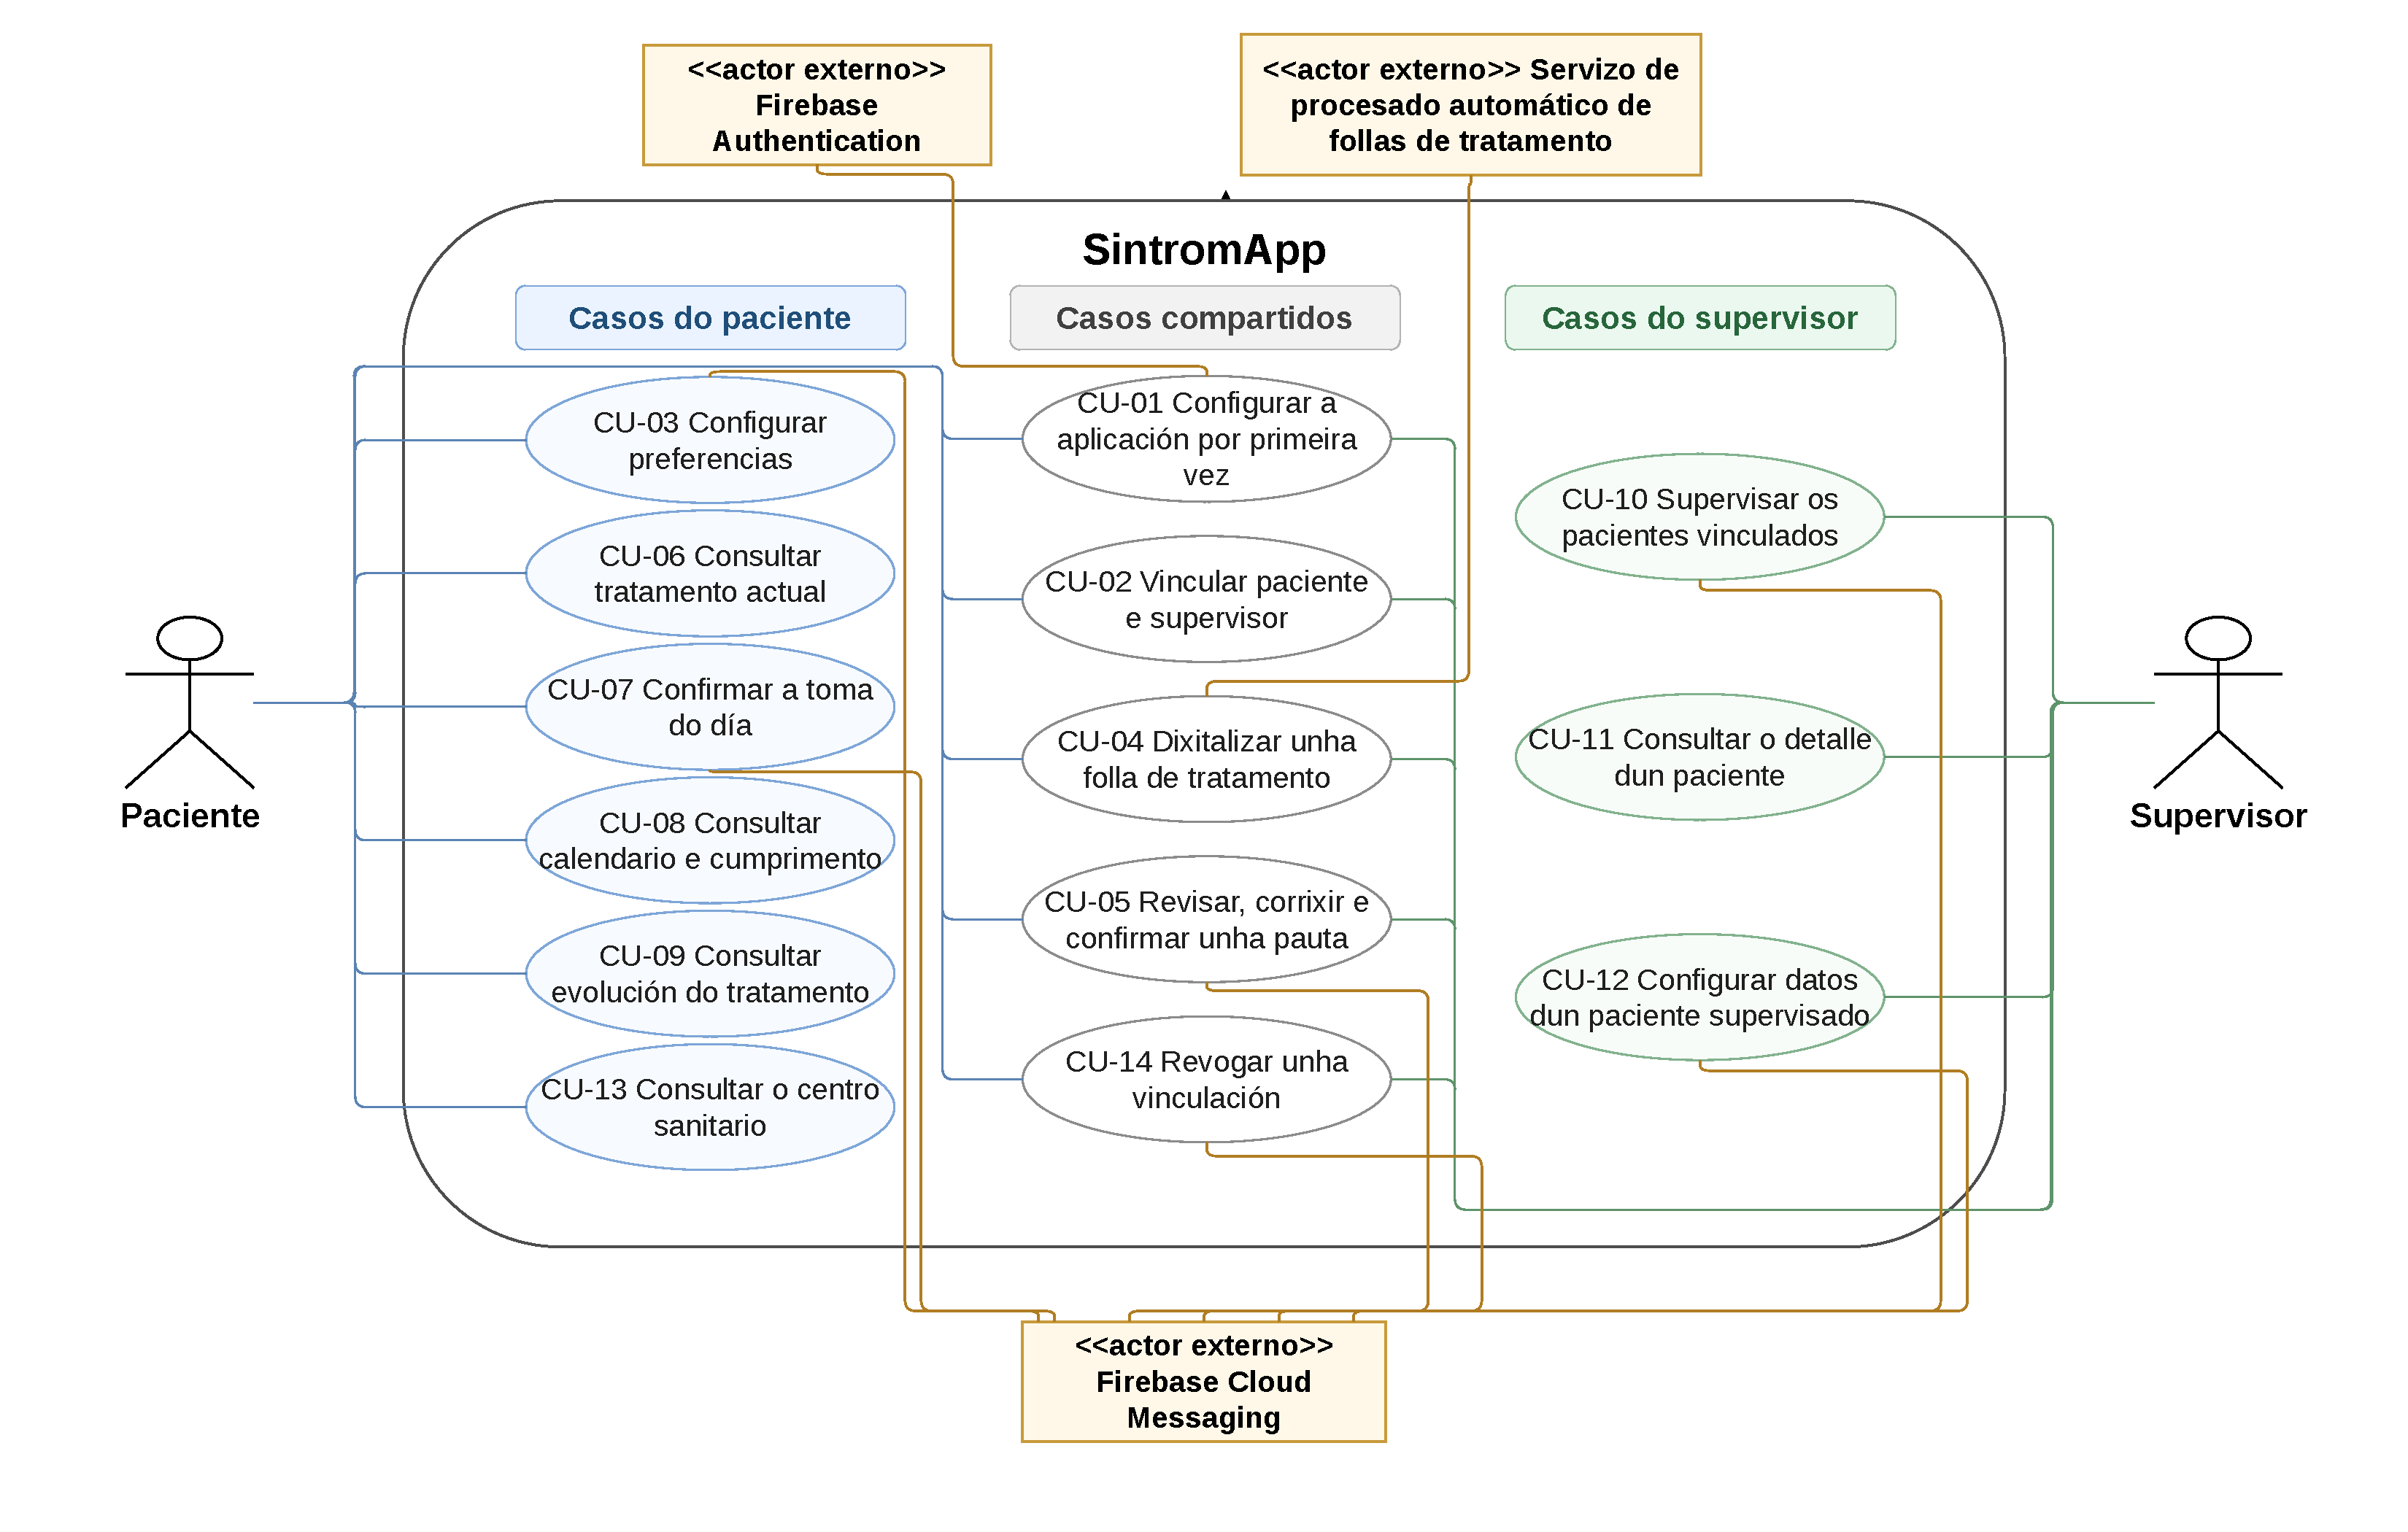
\includegraphics[width=1\linewidth]{imaxes/04-Analise/diagrama_casos_uso_sintromapp_definitivo_letra_moi_grande.drawio.pdf}
\caption{Diagrama dos casos de uso da aplicación}
\label{fig:diagrama-casos-uso}
\end{figure}

 \chapter{Planificación e seguimento}
\label{chap:planificacion}

Neste capítulo preséntanse a planificación temporal e económica do proxecto, comparando a estimación inicial coa evolución real e analizando as principais desviacións e custos.

\section{Planificación inicial}
De acordo co enfoque incremental descrito no Capítulo \ref{chap:metodoloxia}, o proxecto organizouse en sete incrementos. Cada un deles produciu un resultado concreto sobre o que se puido continuar traballando:

\begin{enumerate}
    \item \textbf{Estudo da viabilidade e investigación de tecnoloxías de extracción automática (15 h):}
    análise das follas de tratamento, identificación da información relevante e estudo das posibles técnicas de visión artificial, recoñecemento óptico de caracteres e procesamento documental.

    \item \textbf{Experimentación e selección da tecnoloxía de extracción (45 h):}
    avaliación das alternativas consideradas e selección da tecnoloxía máis adecuada segundo a calidade da extracción, as súas limitacións e a facilidade de integración.

    \item \textbf{Primeira versión da API (35 h):}
    desenvolvemento dunha proba de concepto capaz de recibir unha folla, invocar o servizo de extracción, procesar o resultado e devolver os datos estruturados.

    \item \textbf{Reorganización da API por capas (20 h):}
    separación dos puntos de entrada, a lóxica de negocio, os modelos de datos e as dependencias externas, incorporando tamén as primeiras probas da API.

    \item \textbf{Primeira versión da aplicación Flutter (100 h):}
    implementación progresiva da configuración inicial, os roles de paciente e supervisor, a persistencia, a incorporación de follas, o calendario e o seguimento das tomas.

    \item \textbf{Integración e estabilización (35 h):}
    conexión da aplicación coa \gls{api} e Firebase, incorporación da vinculación, a sincronización e os recordatorios, e estabilización do sistema mediante probas e corrección de erros.

    \item \textbf{Documentación e entrega (50 h):}
    elaboración e revisión da memoria, dos diagramas e dos materiais necesarios para a entrega e presentación do proxecto.
\end{enumerate}

A planificación inicial comezou o 15 de outubro de 2025 e distribuíu un total de 300 horas entre os sete incrementos descritos anteriormente. Como data interna de finalización do proxecto fixouse o 31 de xullo de 2026, co obxectivo de ter rematados tanto o desenvolvemento como a memoria. A data oficial de entrega mantívose no 11 de setembro de 2026. A planificación temporal completa represéntase no diagrama de Gantt da Figura~\ref{fig:gantt-planificacion-inicial}.

\begin{figure}[h]
    \centering
    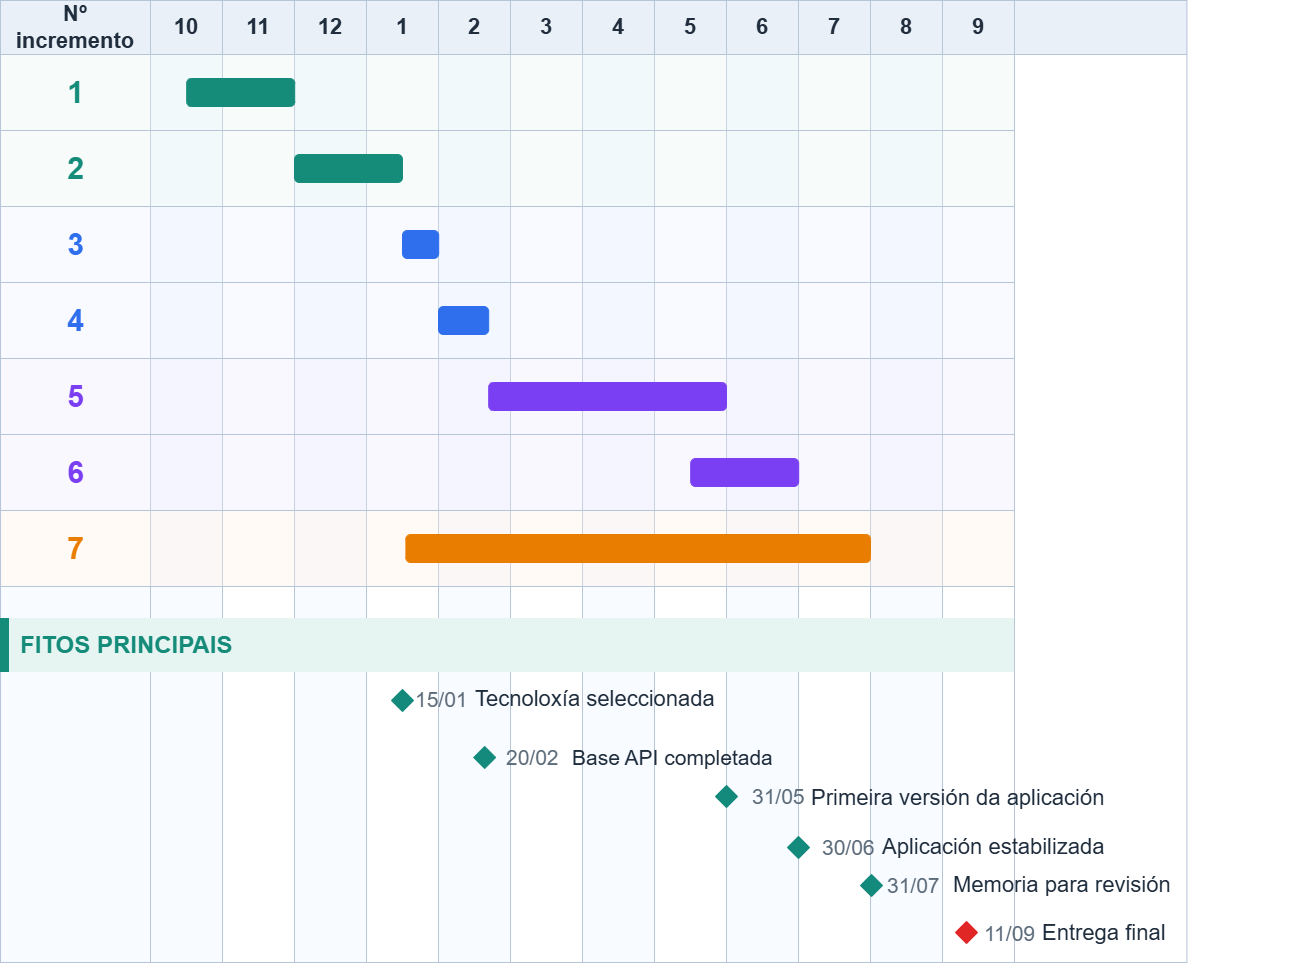
\includegraphics[width=0.75\textwidth]{imaxes/05-Planificacion/gantt-inicial-compacto.drawio.png}
    \caption{Diagrama de Gantt da planificación inicial do proxecto.}
    \label{fig:gantt-planificacion-inicial}
\end{figure}

%ooooooooooooooooooooooooooooooooooooooooooooooooooooooooooooooooooooooooooooooooooooooooooooooooooooo
% HASTA AQUI REVISADO E GUAY
\section{Seguimento e evolución do proxecto}
\label{sec:seguimento-evolucion}

Tal e como se indicou no Capítulo~\ref{chap:metodoloxia}, o control do avance diario levouse a cabo mediante un taboleiro Kanban. Esta xestión visual facilitou o seguimento continuo das tarefas e permitiu adaptar o calendario e a carga de traballo á realidade do desenvolvemento.

Á par desta actualización do calendario, tamén se reavaliou o esforzo necesario. A medida que se avanzaba nas tarefas e se resolvían os primeiros imprevistos, fíxose evidente que a estimación inicial de 300 horas non sería suficiente. Tras revisar a carga de traballo realizada, o historial de confirmacións (\textit{commits}) no repositorio e as métricas do taboleiro Kanban, a dedicación final fixouse nun total de 390 horas (Táboa~\ref{tab:comparacion-horas}). 

\begin{table}[h]
    \centering
    \renewcommand{\arraystretch}{1.2}
    \caption{Comparación entre a dedicación inicial e a dedicación final por incremento.}
    \label{tab:comparacion-horas}
    \small 
    \begin{tabular}{lrrr}
        \toprule
        \textbf{Incremento} &
        \textbf{Inicial (h)} &
        \textbf{Final (h)} &
        \textbf{Diferenza (h)} \\
        \midrule
        Viabilidade e investigación & 15 & 25 & +10 \\
        Experimentación e selección & 45 & 70 & +25 \\
        API inicial & 35 & 45 & +10 \\
        API por capas & 20 & 25 & +5 \\
        Aplicación Flutter & 100 & 125 & +25 \\
        Integración e estabilización & 35 & 50 & +15 \\
        Documentación e entrega & 50 & 50 & 0 \\
        \midrule
        \textbf{Total} & \textbf{300} & \textbf{390} & \textbf{+90} \\
        \bottomrule
    \end{tabular}
\end{table}

Esta cifra supón un incremento de 90 horas, equivalente ao 30\,\% sobre a liña base, e constitúe unha avaliación fundamentada da dedicación real requirida polo proxecto. As causas desta desviación analízanse a continuación.

\subsection{Análise das desviacións}
\label{subsec:analise-desviacions}

A planificación inicial sufriu varias desviacións durante o desenvolvemento. A fase de investigación e experimentación prolongouse pola dificultade para recompilar follas de tratamento e pola necesidade de avaliar distintas tecnoloxías antes de seleccionar unha alternativa fiable. Na \gls{api} foi necesario dedicar máis tempo do previsto ao procesamento e á validación dos datos extraídos, mentres que no cliente móbil a incorporación e revisión de funcionalidades, a integración dos compoñentes e a corrección dos problemas detectados aumentaron tamén a carga de traballo.

A estas desviacións sumouse o cambio na dispoñibilidade horaria. Desde o 17 de marzo de 2026, co inicio das prácticas en empresa, o traballo no proxecto quedou principalmente limitado ás tardes e ás fins de semana e tivo que compaxinarse co resto das materias. Como consecuencia, non se acadou o obxectivo interno de finalizar o proxecto antes do verán, a estabilización prolongouse ata o 15 de agosto e a memoria ata o 31 de agosto, mantendo en todo caso marxe respecto da entrega oficial do 11 de setembro de 2026. O resultado final da planificación móstrase na Figura~\ref{fig:gantt-final}.

\begin{figure}[h]
  \centering
   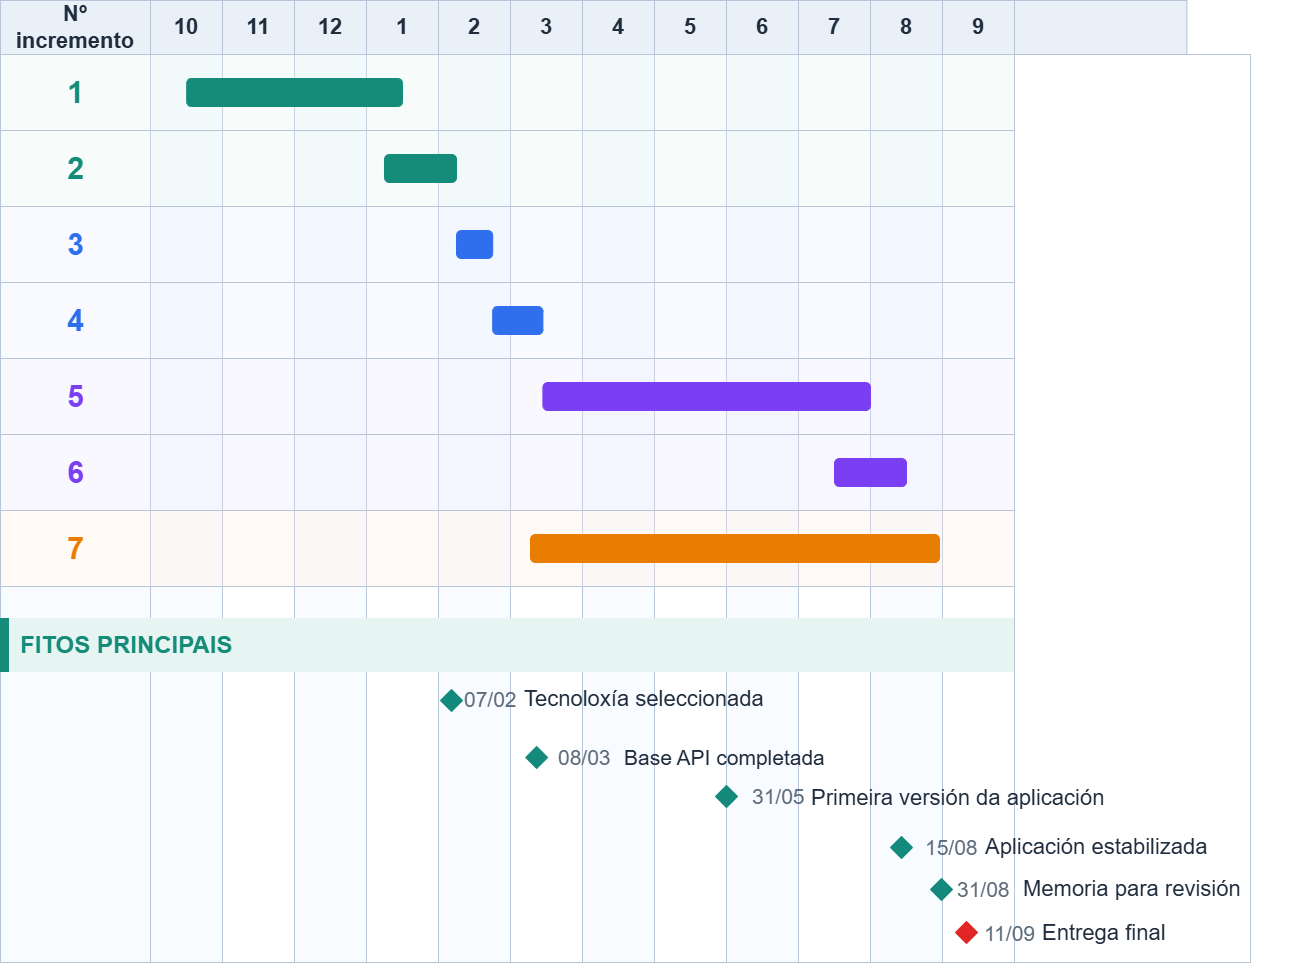
\includegraphics[width=0.75\linewidth]{imaxes/05-Planificacion/gantt-revisado-compacto.drawio.png}
   \caption{Diagrama de Gantt da planificación final do proxecto.}
   \label{fig:gantt-final}
\end{figure}


\section{Custos}
\label{sec:custos-iniciais-revisados}

Para valorar economicamente o esforzo dedicado ao proxecto, tomouse como referencia o salario dun perfil técnico con pouca experiencia segundo o vixente convenio do sector TIC~\cite{BOEConvenioTIC2025}. Partindo dun salario bruto anual de 24.105,37~€~\cite{BOETablasTIC2026} e dunha xornada laboral estándar de 1.800 horas para o ano 2026, obtívose un custo aproximado de 13,39~€/h:

\[
    C_{\mathrm{hora}} =
    \frac{24.105{,}37\ \text{€}}{1.800\ \mathrm{h}}
    \approx 13{,}39\ \text{€/h}
\]

Aplicando este custo á planificación inicial de 300 horas, a valoración prevista do traballo era de 4.017,00~€. A dedicación final ascendeu a 390 horas, polo que a valoración correspondente aumentou ata os 5.222,10~€. Isto supón unha diferenza de 1.205,10~€, derivada das 90 horas adicionais empregadas durante o desenvolvemento.

O hardware necesario xa estaba dispoñible e os servizos e ferramentas empregados utilizáronse mediante créditos de estudante ou modalidades gratuítas. En consecuencia,o desembolso directo foi de 0 € e a desviación económica procede unicamente da valoración das 90 horas adicionais.

 \chapter{Procesamento automático das follas de tratamento}
\label{chap:procesamento-follas}

Unha das funcionalidades principais do sistema é a extracción automática da información contida nas follas de tratamento a partir dunha imaxe. O documento non está formado por texto continuo, senón que distribúe a información en diferentes seccións e táboas. Por este motivo, non é suficiente con recoñecer caracteres de maneira illada, tamén é necesario conservar a relación entre os campos e, especialmente, entre as datas e as doses da pauta diaria.

O procesamento destas follas presenta varias dificultades. En primeiro lugar, a información está organizada mediante campos illados, táboas, valores numéricos e representacións gráficas das doses. A táboa da pauta diaria resulta especialmente relevante, xa que os sistemas de recoñecemento poden identificar correctamente algúns dos seus elementos sen manter a organización en filas e columnas necesaria para asociar cada data coa súa dose.

En segundo lugar, existe unha variabilidade importante nas imaxes de entrada. O uso previsto da aplicación consiste en fotografar a folla mediante un dispositivo móbil, polo que a iluminación, a distancia, o encadramento ou a orientación poden variar entre capturas.

Finalmente, a información procesada é especialmente sensible. Un erro na identificación dunha data ou dunha dose podería provocar que a aplicación mostrase unha pauta incorrecta. Por este motivo, a capacidade de conservar correctamente a relación entre ambos elementos constitúe un dos principais criterios empregados durante a avaliación.

Co obxectivo de determinar unha aproximación adecuada para este problema, estudáronse diferentes técnicas de recoñecemento óptico de caracteres, detección de obxectos e procesamento documental. En concreto, avaliáronse Google ML Kit, Tesseract, unha aproximación baseada na combinación de YOLO cun motor OCR e dous tipos de modelos personalizados de Azure Document Intelligence. Ademais, desenvolveuse unha etapa de preprocesamento mediante OpenCV destinada a corrixir fotografías nas que a folla aparece inclinada ou deformada pola perspectiva.


% ============================================================
% MATERIAIS
% ============================================================

\section{Materiais}
\label{sec:materiais-procesamento}

\subsection{Conxunto de documentos}

Para realizar a experimentación recompilouse un conxunto formado por \textbf{11 follas de tratamento diferentes}. Antes de ser empregadas, eliminouse a información persoal que permitía identificar as persoas pacientes.

As follas manteñen unha estrutura xeral común, aínda que presentan variacións nos datos das visitas, nas datas, nas doses e na distribución dalgúns elementos. En particular, a táboa de doses pode conter representacións gráficas de fraccións de pastilla, valores numéricos e indicacións textuais como \textit{NO TOMAR} ou \textit{CONTROL}.

Cómpre diferenciar entre o número de documentos e o número de imaxes empregado durante as probas. O conxunto está formado por 11 follas diferentes, pero de cada unha delas obtivéronse varias imaxes en condicións distintas. Deste modo, foi posible estudar tanto o comportamento ante documentos diferentes como a influencia das condicións de captura sobre unha mesma folla.


\subsection{Condicións de captura}
\label{sub:cond-cap}

De cada unha das 11 follas obtivéronse \textbf{catro imaxes} baixo condicións de captura diferentes. Esta parte do conxunto está formada, polo tanto, por un total de \textbf{44 imaxes}.

As condicións consideradas foron as seguintes:

\begin{itemize}
    \item unha imaxe escaneada, considerada como caso ideal ou de referencia,
    \item unha fotografía realizada cunha iluminación adecuada,
    \item unha fotografía realizada cun nivel de iluminación inferior,
    \item unha fotografía tomada desde unha distancia maior, de forma que a folla ocupa unha proporción menor da imaxe.
\end{itemize}

Estas variacións pretenden representar situacións que poden producirse durante o uso real da aplicación, no que non se pode garantir que todas as fotografías se realicen cunha iluminación, distancia ou encadramento idénticos.

Adicionalmente, preparouse un subconxunto formado por \textbf{7 fotografías inclinadas}, correspondentes a sete das follas anteriores. Estas imaxes empregáronse especificamente para avaliar a etapa de preprocesamento encargada de corrixir a orientación e, cando é posible identificar os límites da folla, a perspectiva do documento.

Dentro deste subconxunto incluíronse \textbf{dúas fotografías cun fondo claro de tonalidade similar á propia folla}. O obxectivo destes casos foi introducir unha situación máis complexa para a detección do contorno, xa que unha diferenza reducida entre a cor do papel e a do fondo pode dificultar a súa delimitación.

En total, considerando as 44 imaxes correspondentes ás catro condicións de captura e as 7 fotografías inclinadas adicionais, o material preparado para a experimentación está formado por \textbf{51 imaxes obtidas a partir de 11 documentos base}.

A Táboa~\ref{tab:resumo-conxunto-imaxes} resume a composición deste conxunto.

\begin{table}[h!]
    \centering
    \caption{Resumo do conxunto de imaxes empregado na experimentación.}
    \label{tab:resumo-conxunto-imaxes}
    \begin{tabular}{lcc}
        \hline
        \textbf{Condición} &
        \textbf{Documentos} &
        \textbf{Imaxes} \\
        \hline
        Referencia & 11 & 11 \\
        Iluminación adecuada & 11 & 11 \\
        Baixa iluminación & 11 & 11 \\
        Maior distancia & 11 & 11 \\
        Inclinadas & 7 & 7 \\
        \hline
        \textbf{Total} & \textbf{11 diferentes} & \textbf{51} \\
        \hline
    \end{tabular}
\end{table}


\subsection{Distribución dos datos}

A utilización das imaxes variou segundo as necesidades de cada método. Google ML Kit e o modelo estándar de Tesseract non requiriron ningún proceso de adestramento, polo que se aplicaron directamente sobre os documentos seleccionados para cada proba. O conxunto concreto empregado en cada caso indícase posteriormente xunto cos seus resultados.

Nos métodos que si requiriron adestramento realizouse unha división a nivel de documento. As follas \textbf{F01--F08} destináronse ao adestramento, mentres que as follas \textbf{F09--F11} reserváronse exclusivamente para a avaliación. Esta mesma distribución empregouse no modelo personalizado de Tesseract, no detector baseado en YOLO e nos modelos personalizados de Azure Document Intelligence.

Deste modo, ningún exemplo procedente das follas F09--F11 foi empregado durante o adestramento, permitindo avaliar posteriormente os modelos sobre documentos non vistos previamente.

As fotografías inclinadas adicionais empregáronse especificamente para avaliar a etapa de preprocesamento mediante OpenCV.

%A preparación concreta dos datos foi diferente en cada caso. Para Tesseract, as oito follas de adestramento utilizáronse para obter recortes de liñas acompañados da súa transcrición correcta. No caso de YOLO, as imaxes correspondentes a estas follas etiquetáronse manualmente coas rexións que o detector debía localizar. Para Azure Document Intelligence, nas oito follas etiquetáronse os campos considerados de interese para o funcionamento da aplicación.. As tres follas reservadas mantivéronse fóra destes procesos de adestramento e empregáronse posteriormente para comprobar o comportamento sobre documentos non vistos.

% RECOMENDACIÓN:
% Identificar internamente as follas como F01, F02, ..., F11 facilita
% referencialas nas táboas e figuras posteriores.
%
% Por exemplo:
% F01-F08 -> adestramento.
% F09-F11 -> avaliación/proba.
%
% Se finalmente utilizas estes identificadores, mantelos iguais en todo
% o capítulo para poder asociar con claridade cada resultado coa imaxe correspondente.

% TODO:
% Aínda falta indicar o número exacto de recortes xerados para Tesseract
% e, se resulta relevante, o número total de anotacións realizadas en YOLO.


% ============================================================
% MÉTODOS
% ============================================================

\section{Métodos}
\label{sec:metodos-procesamento}

Nesta sección descríbense as diferentes aproximacións exploradas. O obxectivo é explicar o procedemento seguido con cada unha delas e a preparación dos datos necesaria.


% ------------------------------------------------------------
% ML KIT
% ------------------------------------------------------------

\subsection{Google ML Kit}

Para avaliar Google ML Kit, descrito na Sección~\ref{sec:tec-mlkit}, empregouse o seu módulo de recoñecemento de texto co obxectivo de comprobar se a saída xerada podía servir como base para interpretar automaticamente a folla de tratamento.

Desenvolveuse unha pequena aplicación en Flutter que permitía seleccionar unha imaxe almacenada no dispositivo ou capturar unha fotografía da folla e enviala ao recoñecedor de texto de ML Kit.

Como resultado, a ferramenta devolvía o texto detectado xunto coa súa organización en bloques, liñas e elementos. Esta información gardouse en formato JSON para facilitar a análise posterior da orde na que se devolvían os diferentes elementos do documento.

O proceso seguido pola aplicación represéntase na Figura~\ref{fig:secuencia-mlkit}.

\begin{figure}[h!]
    \centering
    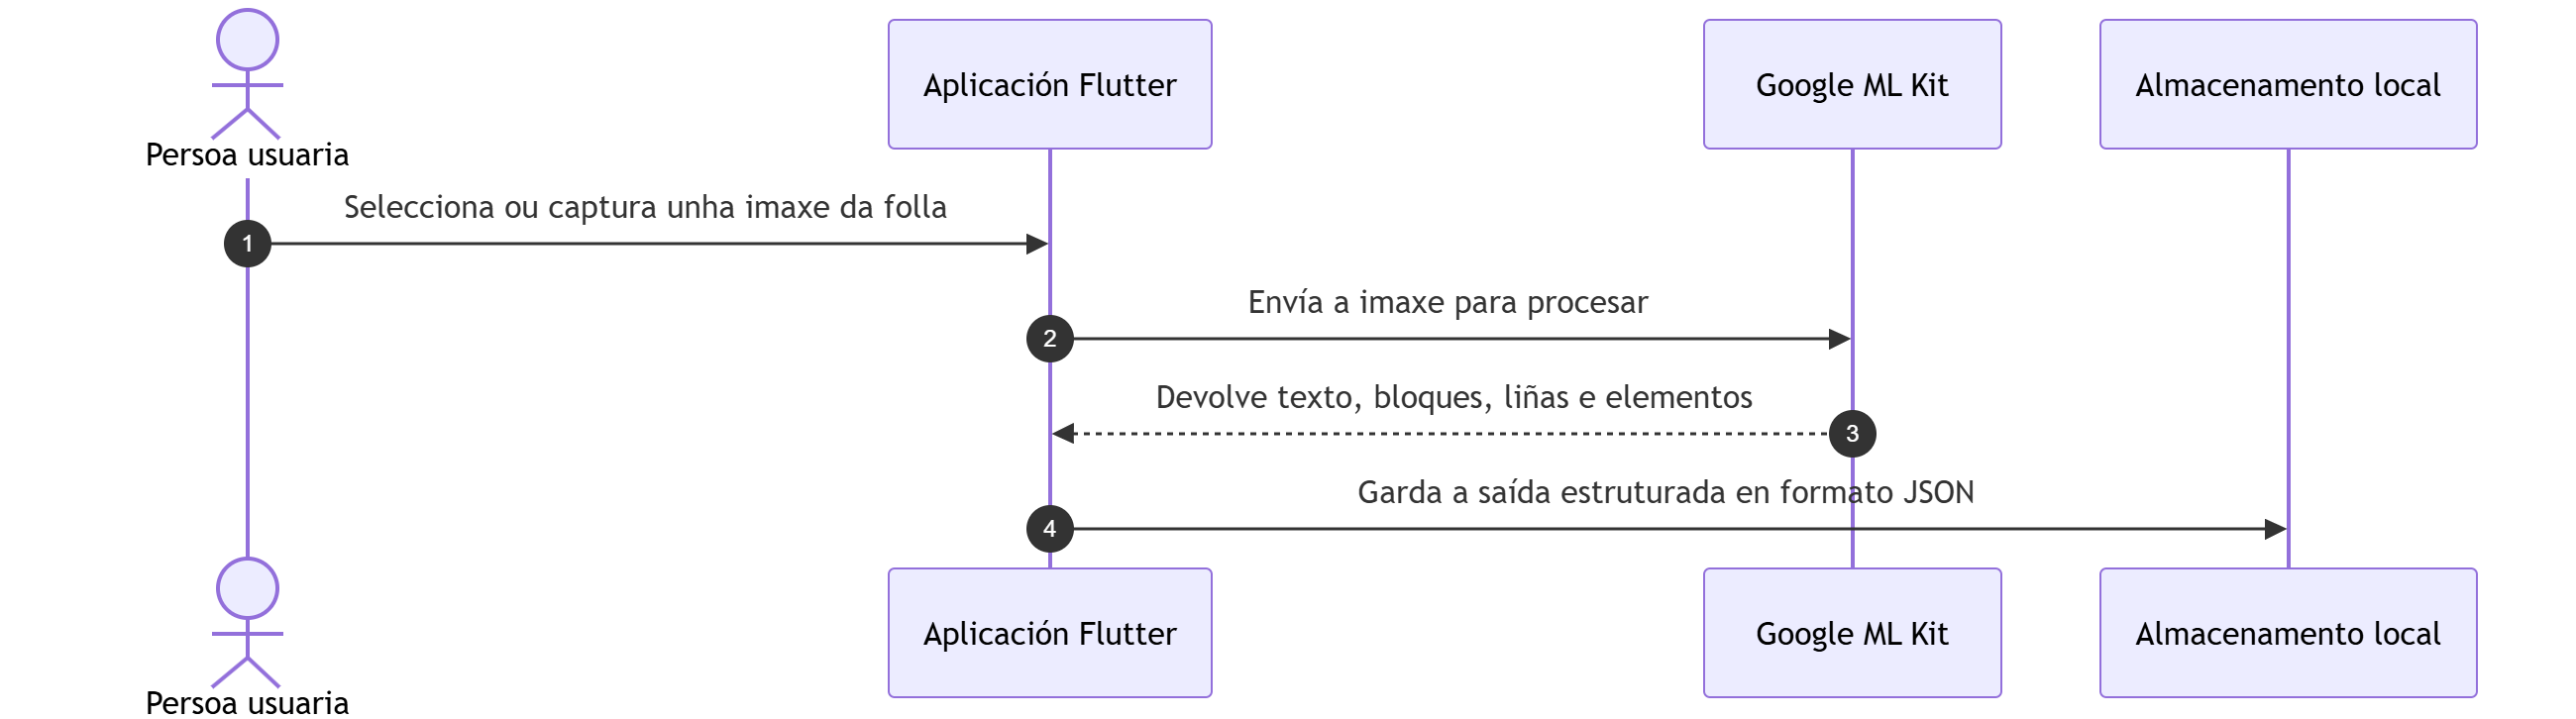
\includegraphics[width=0.9\linewidth]
    {imaxes/06-Procesamento automático das follas de tratamento/mermaid-mlkit.png}
    \caption{Secuencia seguida para procesar unha folla mediante Google ML Kit.}
    \label{fig:secuencia-mlkit}
\end{figure}


% ------------------------------------------------------------
% TESSERACT
% ------------------------------------------------------------

\subsection{Tesseract}

Para avaliar Tesseract, estudáronse dúas variantes, o modelo estándar para lingua española e un modelo personalizado adaptado ao tipo de documento empregado no proxecto.

A primeira proba realizouse empregando o modelo estándar de Tesseract para lingua española, sen introducir ningún proceso de adestramento adicional. As imaxes procesáronse como documentos completos e analizouse directamente a saída textual xerada polo motor OCR. O obxectivo desta proba foi comprobar se un sistema de recoñecemento de texto convencional era capaz de recuperar suficiente información da folla como para reconstruír posteriormente a súa estrutura.

Co obxectivo de adaptar Tesseract á tipografía, ao vocabulario e ao formato das follas de tratamento, construíuse un conxunto de adestramento específico.

Neste caso non se empregaron directamente documentos completos, senón recortes correspondentes a diferentes liñas das follas. Cada exemplo de adestramento estaba formado por dous ficheiros:

\begin{itemize}
    \item un ficheiro con extensión \textit{.png}, que contiña o recorte da liña;
    \item un ficheiro con extensión \textit{.gt.txt}, que contiña o \textit{ground truth}, é dicir, a transcrición correcta do texto presente na imaxe.
\end{itemize}

A partir destes pares realizouse o adestramento dun modelo denominado \textit{sintromv2}. O modelo non se adestrou desde cero, senón que se empregou como punto de partida o modelo español de Tesseract.

O proceso executouse mediante a ferramenta \textit{tesstrain}. O comando empregado foi:

\begin{verbatim}
make training MODEL_NAME=sintromv2 \
    START_MODEL=spa TESSDATA=../tessdata/
\end{verbatim}

Neste comando, \textit{MODEL\_NAME} indica o identificador do novo modelo, \textit{START\_MODEL} especifica o modelo de partida e \textit{TESSDATA} sinala o directorio no que se atopa o ficheiro \textit{spa.traineddata}.

Durante o proceso, \textit{tesstrain} emprega os pares formados pola imaxe e a súa transcrición para adaptar o modelo \gls{lstm} de Tesseract aos exemplos proporcionados.

% ------------------------------------------------------------
% YOLO
% ------------------------------------------------------------

\subsection{Detección de representacións de pastillas mediante YOLO}

A terceira aproximación estudada baseouse no uso de YOLO como detector de obxectos. A diferenza dun sistema OCR, este tipo de modelo non intenta interpretar directamente o texto da imaxe, senón localizar visualmente as rexións correspondentes ás clases que foron definidas durante o adestramento.

A aproximación formulouse en dúas fases. Na primeira, YOLO empregouse para localizar automaticamente as representacións gráficas das pastillas presentes na táboa da pauta. Na segunda, a posición obtida mediante o detector utilizouse como referencia para delimitar unha rexión máis ampla da cela e aplicar posteriormente OCR sobre ese recorte.

%A intención desta estratexia era reducir o problema observado nas aproximacións anteriores: en lugar de solicitar ao motor OCR que interpretase a folla completa e reconstruíse posteriormente a estrutura da táboa, intentábase primeiro localizar os elementos visuais máis característicos e limitar o recoñecemento de texto á súa contorna.

Para a preparación do detector empregouse a ferramenta CVAT, mediante a cal se etiquetaron manualmente as representacións gráficas das pastillas. Esta anotación realizouse baixo unha única clase denominada \textit{pastilla}, debuxando unha caixa delimitadora (bounding box) arredor de cada representación visual. Na Figura~\ref{fig:yolo-cvat} móstrase un exemplo deste proceso.

\begin{figure}[h!]
    \centering
    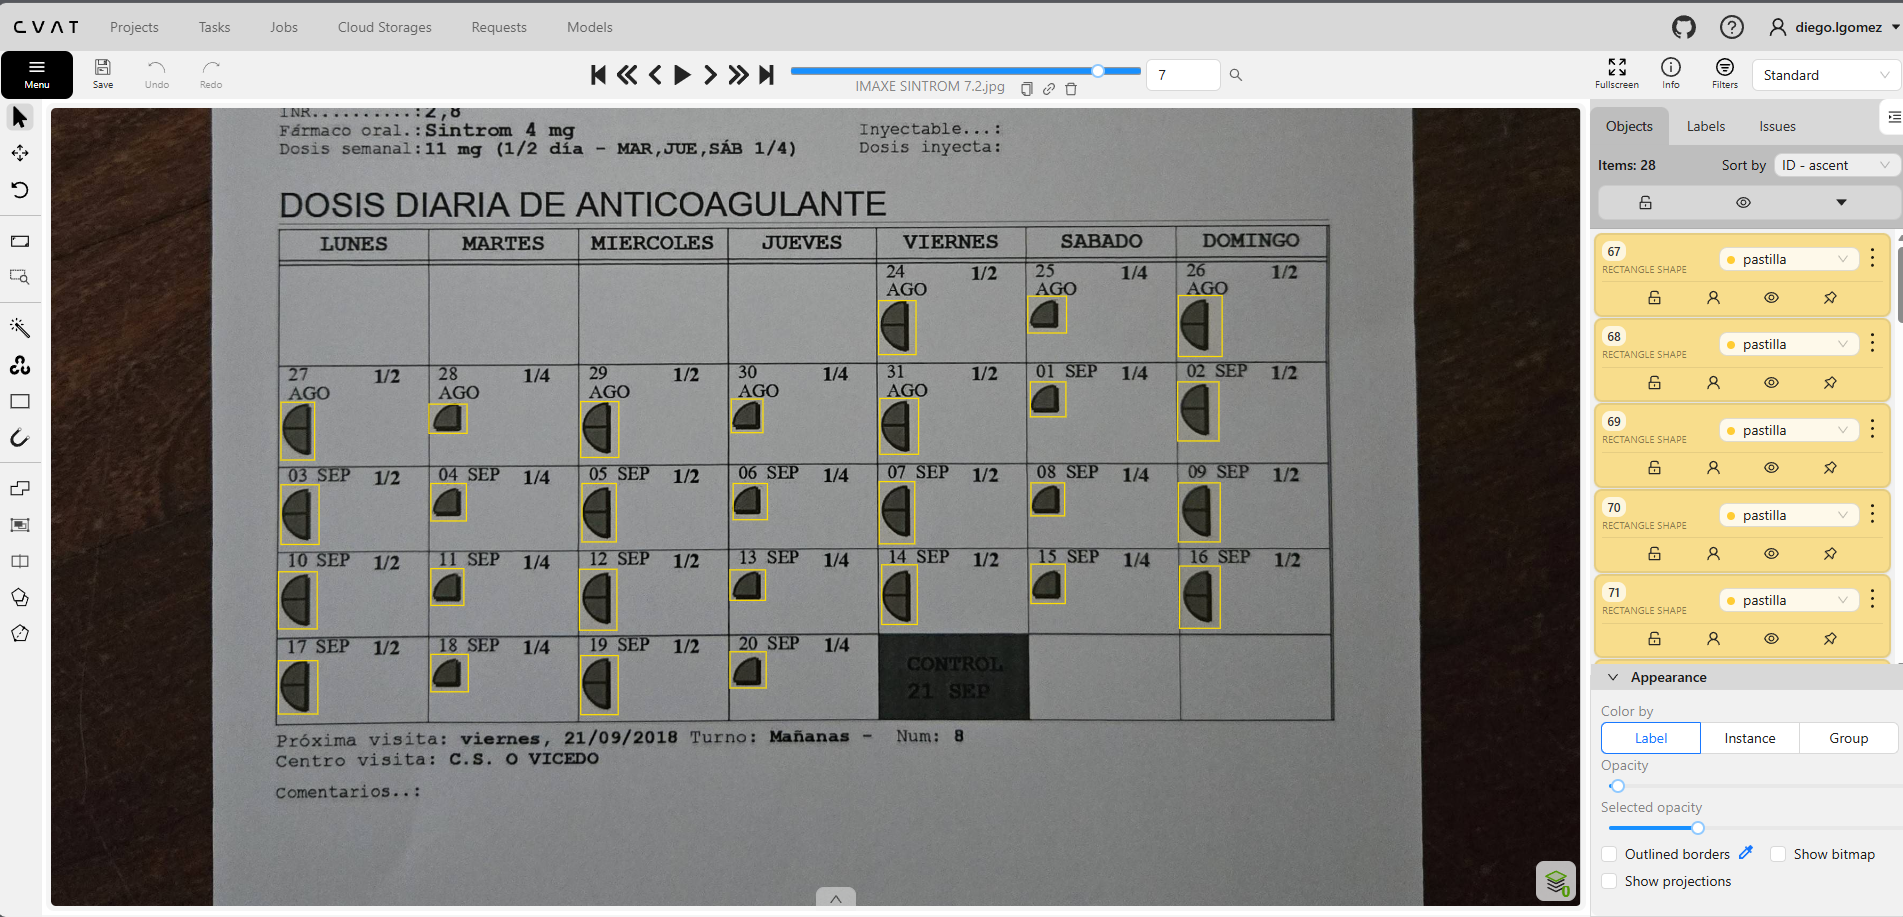
\includegraphics[width=0.85\textwidth]{imaxes/06-Procesamento automático das follas de tratamento/etiquetaxe-CVAT.png}
    \caption{Exemplo de etiquetaxe realizada en CVAT para a detección da clase \textit{pastilla}.}
    \label{fig:yolo-cvat}
\end{figure}

A partir deste conxunto de datos adestrouse un modelo denominado \textit{sintrom\_pastilla}, tomando como punto de partida o modelo preadestrado \textit{yolo11n.pt}. O comando empregado foi:

\begin{verbatim}
yolo detect train data=dataset_pastilla\data.yaml model=yolo11n.pt \
imgsz=1024 epochs=100 batch=4 name=sintrom_pastilla
\end{verbatim}

%Empregouse un tamaño de imaxe de 1024 píxeles debido ao reducido tamaño das representacións das pastillas dentro da folla de tratamento.

Unha vez obtida a detección, ampliouse a rexión delimitada polo modelo para intentar incluír tamén a información asociada á cela e aplicar un OCR sobre o recorte resultante.

Esta segunda fase presenta unha dificultade adicional, xa que a caixa detectada por YOLO corresponde unicamente á representación da pastilla e non aos límites reais da cela. Polo tanto, é necesario decidir canto debe ampliarse a rexión antes de aplicar OCR.

% TODO IMPORTANTE - YOLO + OCR:
%
% Tes que completar esta parte cando acabes as probas.
%
% Explicar:
% 1. Como amplías a bounding box da pastilla.
% 2. Que OCR aplicas finalmente ao recorte.
% 3. Exemplos nos que funciona.
% 4. Exemplos nos que a ampliación inclúe texto doutras celas.
%
% O problema que xa observaches é:
% - a pastilla detéctase ben;
% - ao ampliar a caixa para obter data/dose/cela,
%   ás veces entra información das celas veciñas;
% - ese texto adicional introduce ruído no OCR.
%
% NON concluír aínda aquí se funciona ou non.
% Iso vai na sección de resultados.


% ------------------------------------------------------------
% AZURE DOCUMENT INTELLIGENCE
% ------------------------------------------------------------

\subsection{Azure Document Intelligence}

Para avaliar Azure Document Intelligence optouse por adestrar modelos personalizados capaces de interpretar a estrutura específica das follas de tratamento. 

A partir das necesidades da aplicación definiuse un esquema cos campos que se consideraron relevantes para a extracción, entre eles as datas e doses da pauta diaria, o INR, o fármaco, a seguinte visita e a información correspondente ao histórico de visitas.

Estes campos etiquetáronse manualmente mediante Azure Document Intelligence Studio, asociando en cada documento as rexións correspondentes coas etiquetas definidas no esquema. Na Figura~\ref{fig:etiquetaxe-azure} móstrase un exemplo deste proceso.

\begin{figure}[h!]
    \centering
    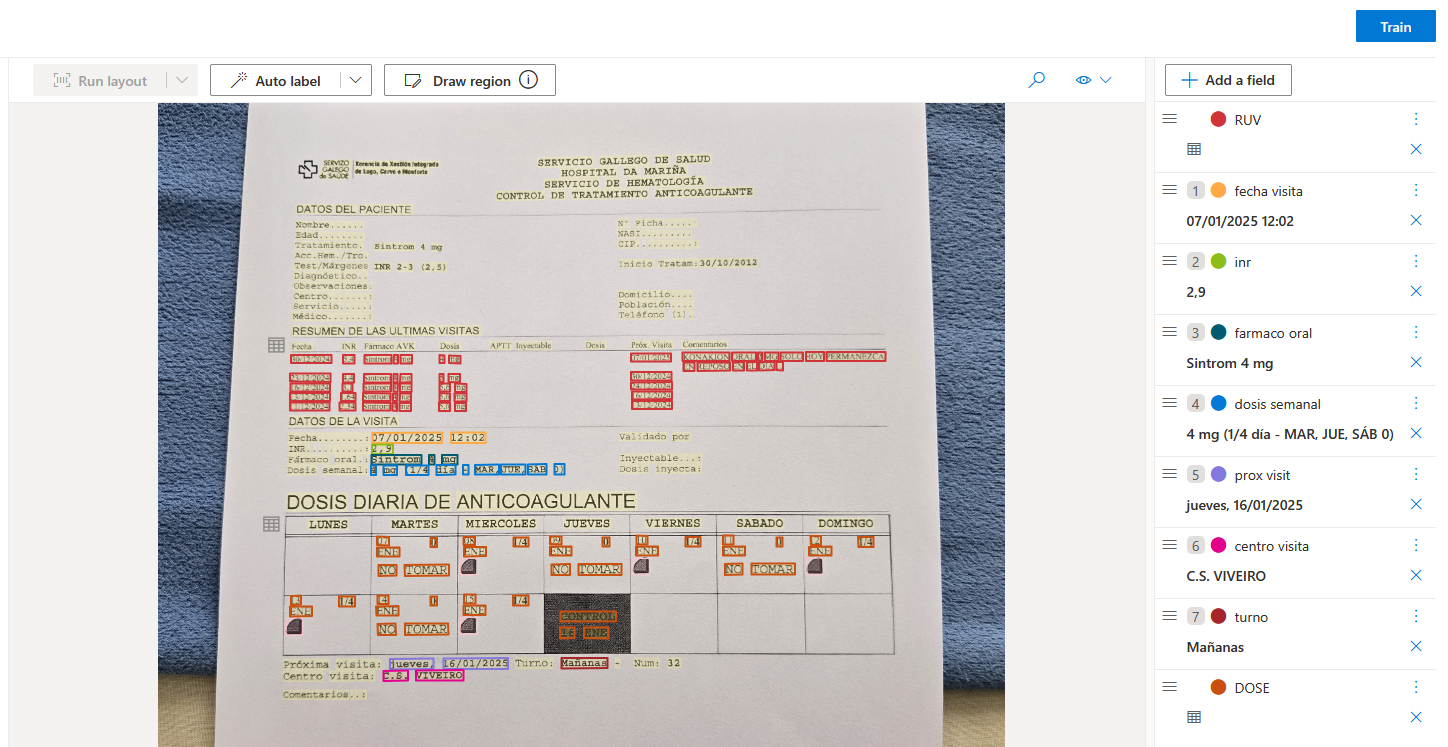
\includegraphics[width=0.9\textwidth]{imaxes/06-Procesamento automático das follas de tratamento/EtiquetaxeAzure.png}
    \caption{Interface de etiquetaxe en Azure Document Intelligence Studio.}
    \label{fig:etiquetaxe-azure}
\end{figure}

A partir do mesmo conxunto de documentos etiquetados adestráronse dous modelos personalizados, empregando as arquitecturas \textit{Neural} e \textit{Template}. A primeira está baseada en técnicas de aprendizaxe profunda e está orientada a documentos nos que a disposición e a posición da información poden variar entre exemplos. Esta maior flexibilidade implica tamén unha maior necesidade de datos de adestramento.

Pola súa banda, a arquitectura \textit{Template} baséase principalmente na disposición espacial dos elementos e na repetición de estruturas e patróns xeométricos entre os documentos, polo que está especialmente orientada a formatos cunha organización relativamente estable.

Dado o reducido número de documentos dispoñibles para o adestramento e a estrutura repetitiva das follas de tratamento, adestráronse e avaliáronse ambas arquitecturas co obxectivo de comparar o seu comportamento sobre o mesmo conxunto de datos.

As \textbf{3 follas reservadas para a avaliación}, que non foran empregadas durante o adestramento, utilizáronse para comparar ambas arquitecturas. Deste modo, os dous modelos puideron ser avaliados sobre os mesmos documentos e sobre información non vista previamente.

%METER ICUAL EN IMPLEMENTACION 
\subsection{Preprocesamento das imaxes mediante OpenCV}
\label{sec:preprocesamento-opencv}

Ademais das aproximacións estudadas para a extracción da información, incorporouse unha etapa previa de preprocesamento mediante OpenCV destinada a corrixir as fotografías nas que a folla aparece inclinada ou deformada pola perspectiva. Esta etapa non realiza a extracción dos datos, senón que prepara a imaxe antes de enviala ao sistema encargado do seu procesamento.

O procedemento deseñouse seguindo un criterio conservador: a imaxe só se modifica cando se detecta cun nivel suficiente de confianza que é necesaria unha corrección. En caso contrario, mantense a imaxe orixinal para evitar que unha transformación incorrecta poida eliminar ou deformar información relevante.

O proceso comeza coa detección dos bordos e dos principais contornos da imaxe, tratando de identificar a folla como unha rexión cuadrangular. Tamén se contempla unha segunda estratexia baseada na detección de superficies claras, pensada para fotografías nas que os límites do papel resultan menos evidentes. Cando se localizan de maneira fiable os catro extremos da folla, aplícase unha transformación de perspectiva que permite obter unha vista frontal do documento e eliminar parte do fondo exterior.

Se non é posible delimitar completamente a folla, emprégase unha alternativa baseada na orientación das liñas detectadas no documento. A partir delas estímase o ángulo de inclinación e, cando a desviación é significativa, rótase a fotografía para aliñala. Se non existe suficiente evidencia para aplicar ningunha das dúas correccións, a entrada continúa sen modificacións.

Esta etapa integrouse antes do proceso de extracción da API, de forma que o sistema encargado de interpretar o documento recibe a versión corrixida cando é necesario. Para avaliar especificamente este mecanismo preparouse un subconxunto de \textbf{7 fotografías inclinadas}, correspondentes a sete documentos diferentes. Dúas delas realizáronse sobre fondos claros similares á propia folla co obxectivo de comprobar o comportamento da detección en condicións de menor contraste.

% FIGURA RECOMENDADA:
% Nos resultados, mostrar:
% (a) imaxe inclinada orixinal;
% (b) resultado corrixido;
% (c) imaxe sobre fondo claro;
% (d) resultado correspondente.


% ============================================================
% CRITERIOS DE AVALIACIÓN
% ============================================================

\section{Criterios de avaliación}
\label{sec:criterios-avaliacion-procesamento}

Unha vez descritas as diferentes aproximacións, establecéronse os aspectos empregados para analizar os resultados obtidos e determinar a súa adecuación ao problema.

A avaliación centrouse principalmente nos seguintes criterios:

\begin{itemize}
    \item a capacidade de recoñecer correctamente texto, datas e valores numéricos;
    \item a conservación da estrutura das táboas;
    \item a asociación entre cada data e a súa dose correspondente;
    \item a estabilidade e facilidade de interpretación do formato de saída;
    \item o esforzo necesario para preparar e etiquetar os datos;
    \item o comportamento ante diferentes condicións de captura.
\end{itemize}

A táboa de doses considerouse o elemento máis importante da avaliación, xa que constitúe a base a partir da cal a aplicación representa a pauta diaria e programa os avisos correspondentes. Por este motivo, non se considerou suficiente que unha tecnoloxía recoñecese correctamente palabras ou números de maneira independente. Para resultar adecuada debía ser posible determinar de forma fiable que dose correspondía a cada data.

No caso da aproximación baseada en YOLO, valorouse adicionalmente a capacidade de localizar as representacións gráficas das pastillas e a posibilidade de utilizar esas deteccións como punto de partida para delimitar a información da cela correspondente.

No caso concreto da etapa de preprocesamento mediante OpenCV, a avaliación centrouse en comprobar se era posible detectar unha inclinación significativa, endereitar correctamente o documento e, cando se identificaban os seus catro bordos, corrixir tamén a deformación de perspectiva e recortar as zonas exteriores innecesarias.

Ao mesmo tempo, considerouse especialmente importante comprobar que unha fotografía xa correctamente aliñada non fose modificada e que, ante unha detección dubidosa, se mantivese a imaxe orixinal en lugar de aplicar unha transformación potencialmente incorrecta.

%REVISAR
Finalmente, unha vez seleccionada unha aproximación para realizar a extracción, avaliouse de forma específica o seu comportamento ante diferentes condicións de iluminación e distancia, xa que estas situacións representan mellor o contexto real no que se utilizará a aplicación.


% ============================================================
% RESULTADOS
% ============================================================

\section{Resultados}
\label{sec:resultados-procesamento}

\subsection{Resultados de Google ML Kit}

A avaliación de Google ML Kit realizouse inicialmente sobre as \textbf{11 follas de tratamento escaneadas}, consideradas como o escenario de referencia e as condicións máis favorables de entrada. O obxectivo desta primeira proba foi comprobar se a ferramenta permitía recuperar non só o texto presente no documento, senón tamén a información necesaria para reconstruír de maneira fiable a pauta de tratamento.

ML Kit conseguiu recoñecer unha parte importante do contido dos documentos. Non obstante, observáronse erros mesmo nestas condicións favorables. Entre os exemplos atopamos, valores de INR como \textit{1,9} e \textit{2,2} foron devoltos como \textit{19} e \textit{22}, respectivamente, e producíronse tamén modificacións en datas, como \textit{11/12/2024} recoñecido como \textit{1/12/2024} ou \textit{25/05/2018} como \textit{2.5/05/2018}.

% FONTES:
% F01.json -> INR 1,9 -> 19
% F10.json -> INR 2,2 -> 22
% F05.json -> 11/12/2024 -> 1/12/2024
% F07.json -> 25/05/2018 -> 2.5/05/2018

A principal limitación atopada apareceu na táboa de doses diarias. A ferramenta recoñece numerosos elementos do seu contido, pero a saída non conserva de maneira estable a estrutura visual da táboa. Entre as distintas imaxes probadas, as entradas aparecen agrupadas parcialmente por columnas ou distribuídas entre bloques diferentes, de modo que o día, o mes e a dose dunha mesma cela non sempre forman unha única secuencia. Como consecuencia, a orde textual obtida non coincide necesariamente coa orde cronolóxica da pauta. Por exemplo, nalgúns casos a dose aparece despois da data, como en \textit{20 DIC 1/4}, noutros sitúase antes, como en \textit{1/4 17 DIC} e tamén se observaron agrupacións como \textit{18 DIC 1/4 19 1/4 DIC}, nas que quedan mesturados elementos pertencentes a entradas distintas.


Esta variabilidade dificulta establecer un formato de saída sobre o que aplicar de maneira fiable patróns ou expresións regulares. As coordenadas proporcionadas por ML Kit poderían empregarse como apoio para reorganizar espacialmente os elementos detectados, pero non resolven os erros producidos no propio recoñecemento. Entre as follas escaneadas atopáronse, por exemplo, \textit{05 ENE} devolto como \textit{0 ENE}, doses \textit{1/2} recoñecidas como \textit{/2} e \textit{16 NOV} interpretado como
\textit{l6 NOV}. Nestes casos parte da información orixinal foi omitida ou substituída, polo que non pode recuperarse de maneira inequívoca mediante unicamente a reorganización dos elementos ou un postprocesamento.

% FONTES:
% F08.json -> 05 ENE -> 0 ENE
% F10.json -> 16 NOV -> l6 NOV
% F10.json -> aparecen doses 1/2 incompletas como /2

Unha vez identificadas estas limitacións nas imaxes de referencia, realizáronse probas adicionais con \textbf{cinco fotografías tomadas con iluminación normal}, co obxectivo de comprobar o comportamento da ferramenta nun escenario máis próximo ao uso real da aplicación. Os problemas estruturais mantivéronse, as entradas da pauta non sempre se devolveron seguindo a súa orde cronolóxica, senón agrupadas parcialmente por columnas e intercaladas con información procedente doutras zonas do documento.

Ademais, continuaron producíndose erros no propio contido recoñecido. Na pauta diaria apareceron repetidamente doses \textit{1/2} devoltas como \textit{/2} ou \textit{12}; tamén se modificaron días, como \textit{11 SEP} recoñecido como \textit{TI SEP}, e nalgún caso chegou a omitirse completamente o número do día, conservándose unicamente o mes e a dose. Fóra da táboa observáronse igualmente erros en campos, como \textit{Sintrom 4 mg} recoñecido como \textit{Sin tromn 4 ng}, así como modificacións en datas e valores numéricos, como \textit{15/01/2025} recoñecido como \textit{JS/01/2025} ou \textit{3,5 mg} como \textit{35 mg}.

% FONTES:
%
% F01-N.json:
% - orde da táboa alterada, con entradas agrupadas parcialmente por columnas
% - 08 SEP 1/2 -> 08 SEP /2
% - 11 SEP 1/2 -> TI SEP 1/2
% - 12 SEP 1/2 -> 12 SEP 12
% - 14 SEP 1/2 -> 14 SEP 12
% - 10 OCT 1/2 -> non se recoñece o número 10; quedan OCT e a dose
%
% F03-N.json:
% - Sintrom 4 mg -> Sin tromn 4 ng
% - 15/01/2025 -> JS/01/2025
% - 3,5 mg -> 35 mg
%
% F07-N.json:
% - tamén aparecen doses 1/2 recoñecidas como /2

A Figura~\ref{fig:mlkit-f01n-entrada} mostra un fragmento dunha das cinco fotografías tomadas con iluminación normal empregadas nestas probas, mentres que o Listing~\ref{lst:mlkit-f01n-saida} recolle a saída bruta xerada por ML Kit para esa mesma imaxe. Nel poden observarse de forma conxunta a perda da estrutura da táboa e os erros de recoñecemento descritos anteriormente.

\begin{figure}[hp!]
    \centering
    % Empregar F01-N.
    % RECOMENDACIÓN: recortar desde
    % "DOSIS DIARIA DE ANTICOAGULANTE"
    % ata o final da primeira fila (08--14 SEP).
    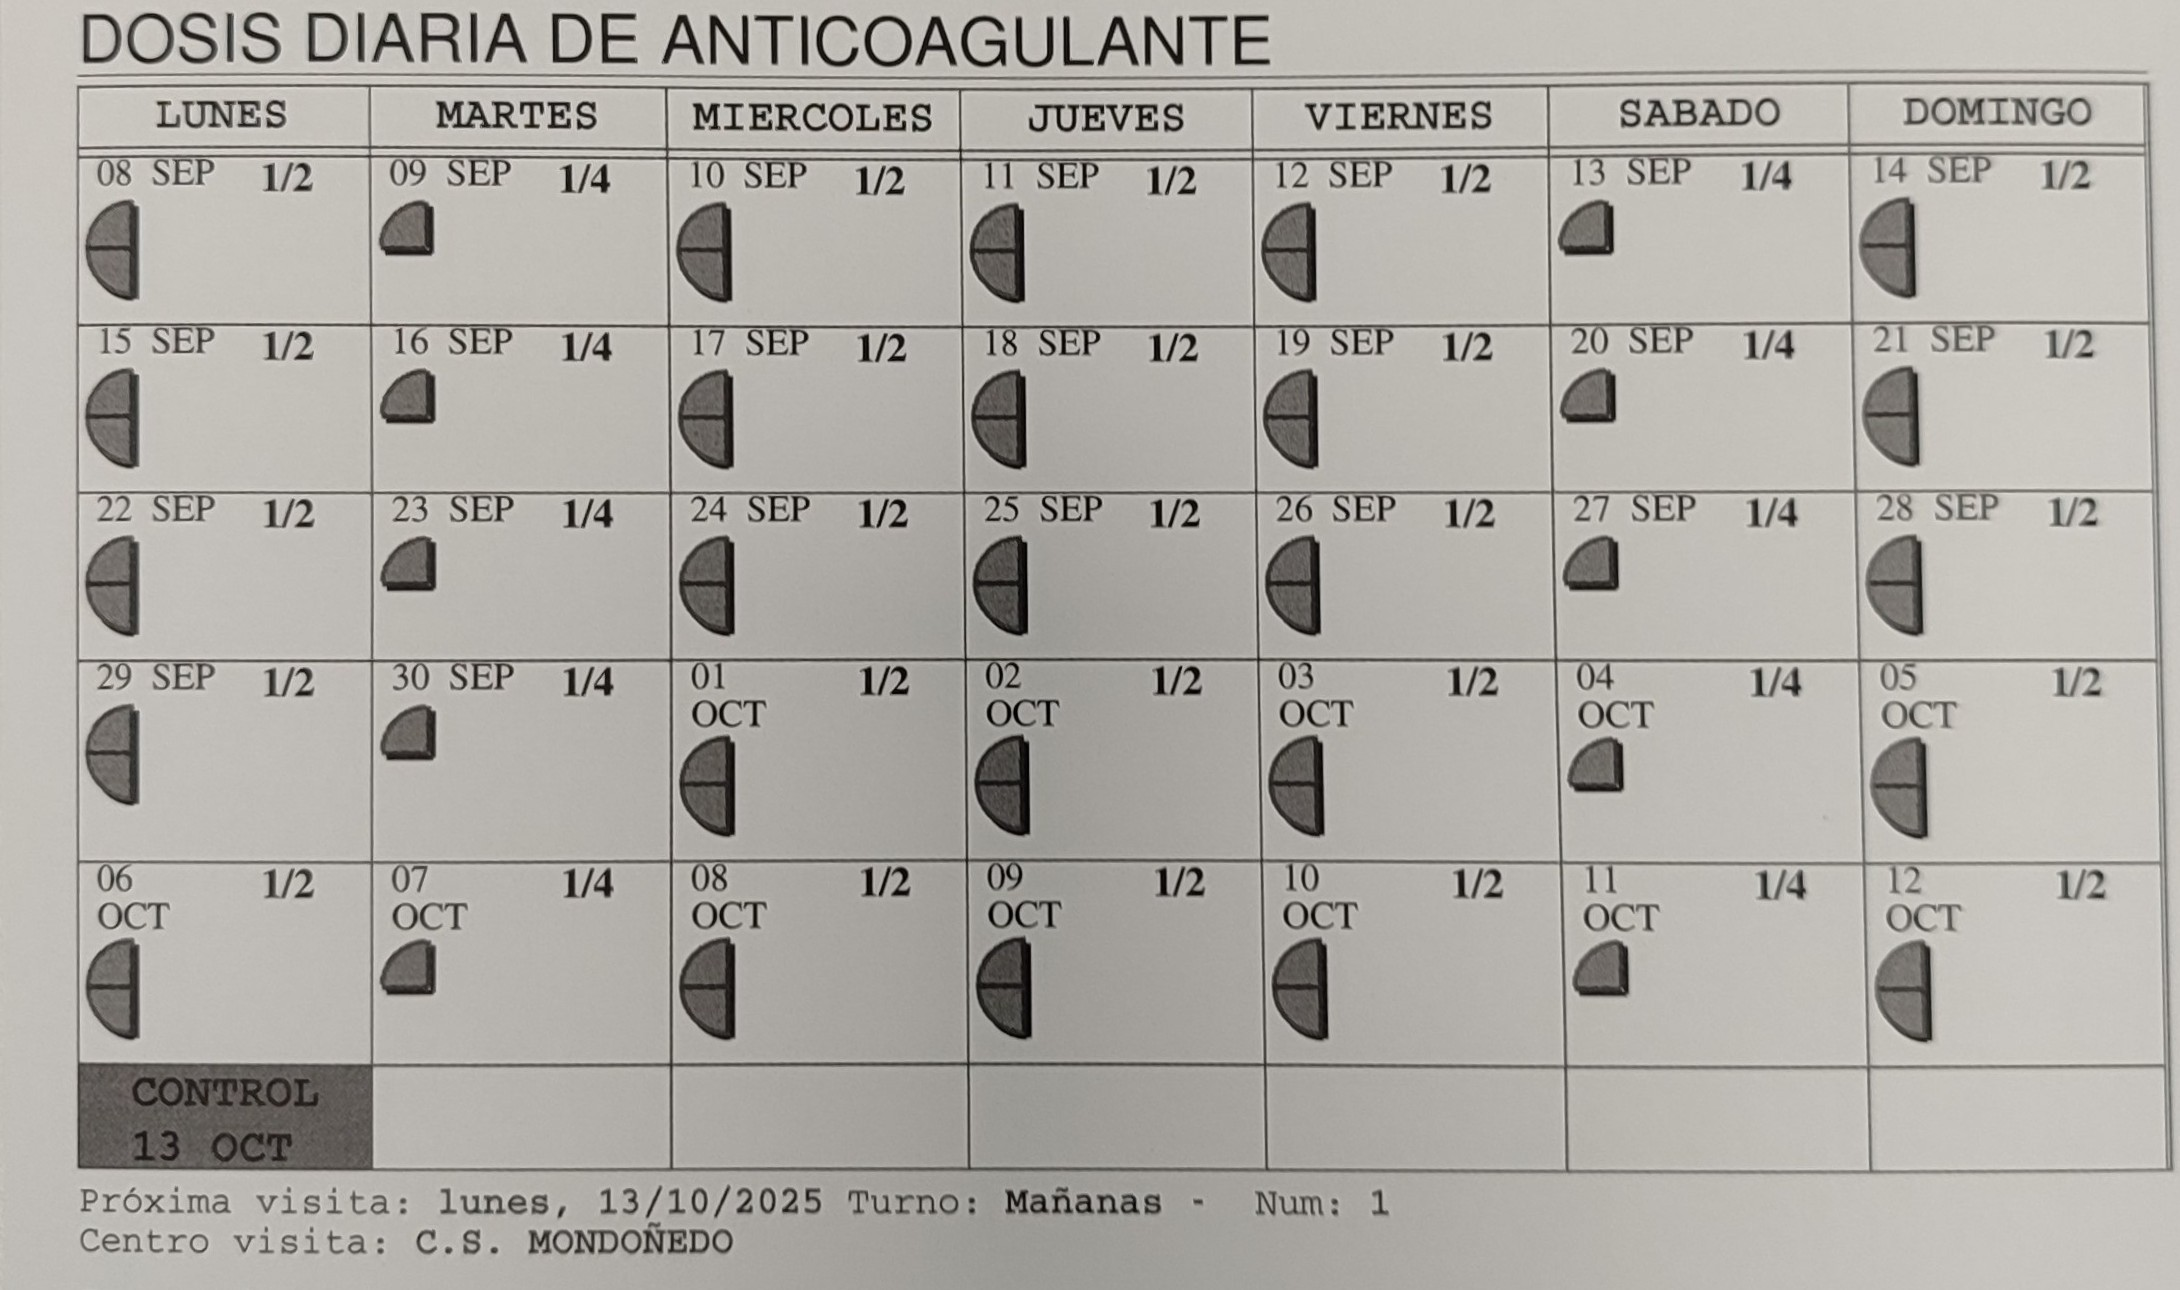
\includegraphics[width=0.75\textwidth]{imaxes/06-Procesamento automático das follas de tratamento/mlkit-f01n-pauta.jpg}
    \caption{Fragmento dunha fotografía tomada con iluminación normal
    empregada na avaliación de Google ML Kit.}
    \label{fig:mlkit-f01n-entrada}
\end{figure}

\begin{lstlisting}[
    frame=single,
    rulecolor=\color{gray!60},
    backgroundcolor=\color{gray!5},
    basicstyle=\ttfamily\scriptsize,
    escapeinside={(*}{*)},
    caption={Fragmento anotado da saída bruta de ML Kit para a fotografía da Figura~\ref{fig:mlkit-f01n-entrada}},
    label={lst:mlkit-f01n-saida},
    captionpos=t,
    columns=fullflexible,
    keepspaces=true
]
VIERNES
(*\textcolor{red}{12 SEP 12}*)   (*\textcolor{red}{$\leftarrow$ 1/2 recoñecido como 12}*)
C.S. MONDONEDO      (*\textcolor{red}{$\leftarrow$ información allea á pauta}*)
19 SEP
26 SEP
03
OCT
(*\textcolor{red}{OCT}*)         (*\textcolor{red}{$\leftarrow$ falta o día 10}*)
Num: 1             (*\textcolor{red}{$\leftarrow$ información doutra zona}*)
1/2
1/2
1/2
1/2                 (*\textcolor{red}{$\leftarrow$ doses separadas das datas}*)

SABADO
13 SEP 1/4
20 SEP
27 SEP
04
OCT
11
OCT
1/4
1/4
1/4
1/4                 (*\textcolor{red}{$\leftarrow$ datas e doses en grupos distintos}*)

DOMINGO
(*\textcolor{red}{14 SEP 12}*)   (*\textcolor{red}{$\leftarrow$ 1/2 recoñecido como 12}*)
21 SEP
28 SEP
05
OCT
[...]
12
OCT
12
12
(*\textcolor{red}{/2}*)          (*\textcolor{red}{$\leftarrow$ perda do numerador}*)
12
\end{lstlisting}

As probas realizadas sobre as \textbf{11 follas escaneadas} e as \textbf{cinco fotografías tomadas con iluminación normal} permitiron avaliar o comportamento de ML Kit tanto en condicións favorables como nun escenario máis próximo ao uso real da aplicación. Os resultados obtidos en ambos os casos mostraron limitacións que afectaban directamente á información necesaria para reconstruír a pauta de tratamento. Por este motivo, non se considerou necesario ampliar a avaliación a outras condicións de captura, xa que a
evidencia recollida resultaba suficiente para descartar a ferramenta como solución principal.

En consecuencia, aínda que Google ML Kit mostrou unha boa capacidade para recoñecer unha parte importante do texto presente nas follas, non proporcionou unha saída suficientemente fiable para reconstruír de forma segura a pauta diaria. Por este motivo, a ferramenta foi descartada como solución principal para a extracción automática.


% ------------------------------------------------------------
% RESULTADOS TESSERACT
% ------------------------------------------------------------

\subsection{Resultados de Tesseract}

\subsubsection{Modelo estándar}

A avaliación do modelo estándar de Tesseract realizouse sobre as \textbf{11 follas de tratamento escaneadas}, empregando o modelo para español \textit{spa}. Ao tratarse das imaxes de referencia, estas probas permitiron analizar o seu comportamento nas condicións de entrada máis favorables antes de considerar escenarios de captura máis complexos.

Tesseract conseguiu recuperar correctamente unha parte do texto xeral dos documentos, especialmente cabeceiras, etiquetas e algúns campos das visitas. Non obstante, os resultados presentaron numerosos erros tipográficos, confusións entre caracteres e modificacións en valores numéricos. Estes problemas afectaron tamén á información relevante para o tratamento. Por exemplo, nunha das follas apareceron valores como \textit{35 me}, \textit{29}, \textit{54} ou \textit{44} en campos nos que os valores orixinais incluían unidades ou separadores decimais. 
% F03.txt

A maior dificultade apareceu novamente na táboa de doses diarias. Aínda que nalgúns documentos se recoñeceron correctamente varias entradas, o comportamento foi moi irregular entre as distintas follas. Observáronse perdas ou modificacións dos separadores das fraccións, días incorrectos, caracteres sen relación co contido da táboa e agrupacións que dificultan establecer a correspondencia entre cada data e a súa dose.

Un dos exemplos máis representativos obsérvase na folla F04. Como mostra o Listing~\ref{lst:tesseract-estandar-f04}, a saída conserva algúns elementos recoñecibles, pero introduce numerosos caracteres incorrectos e perde a estrutura necesaria para asociar de forma fiable cada data coa súa dose.

\begin{figure}[h!]
    \centering
    % Recorte da táboa da folla F01 escaneada.
    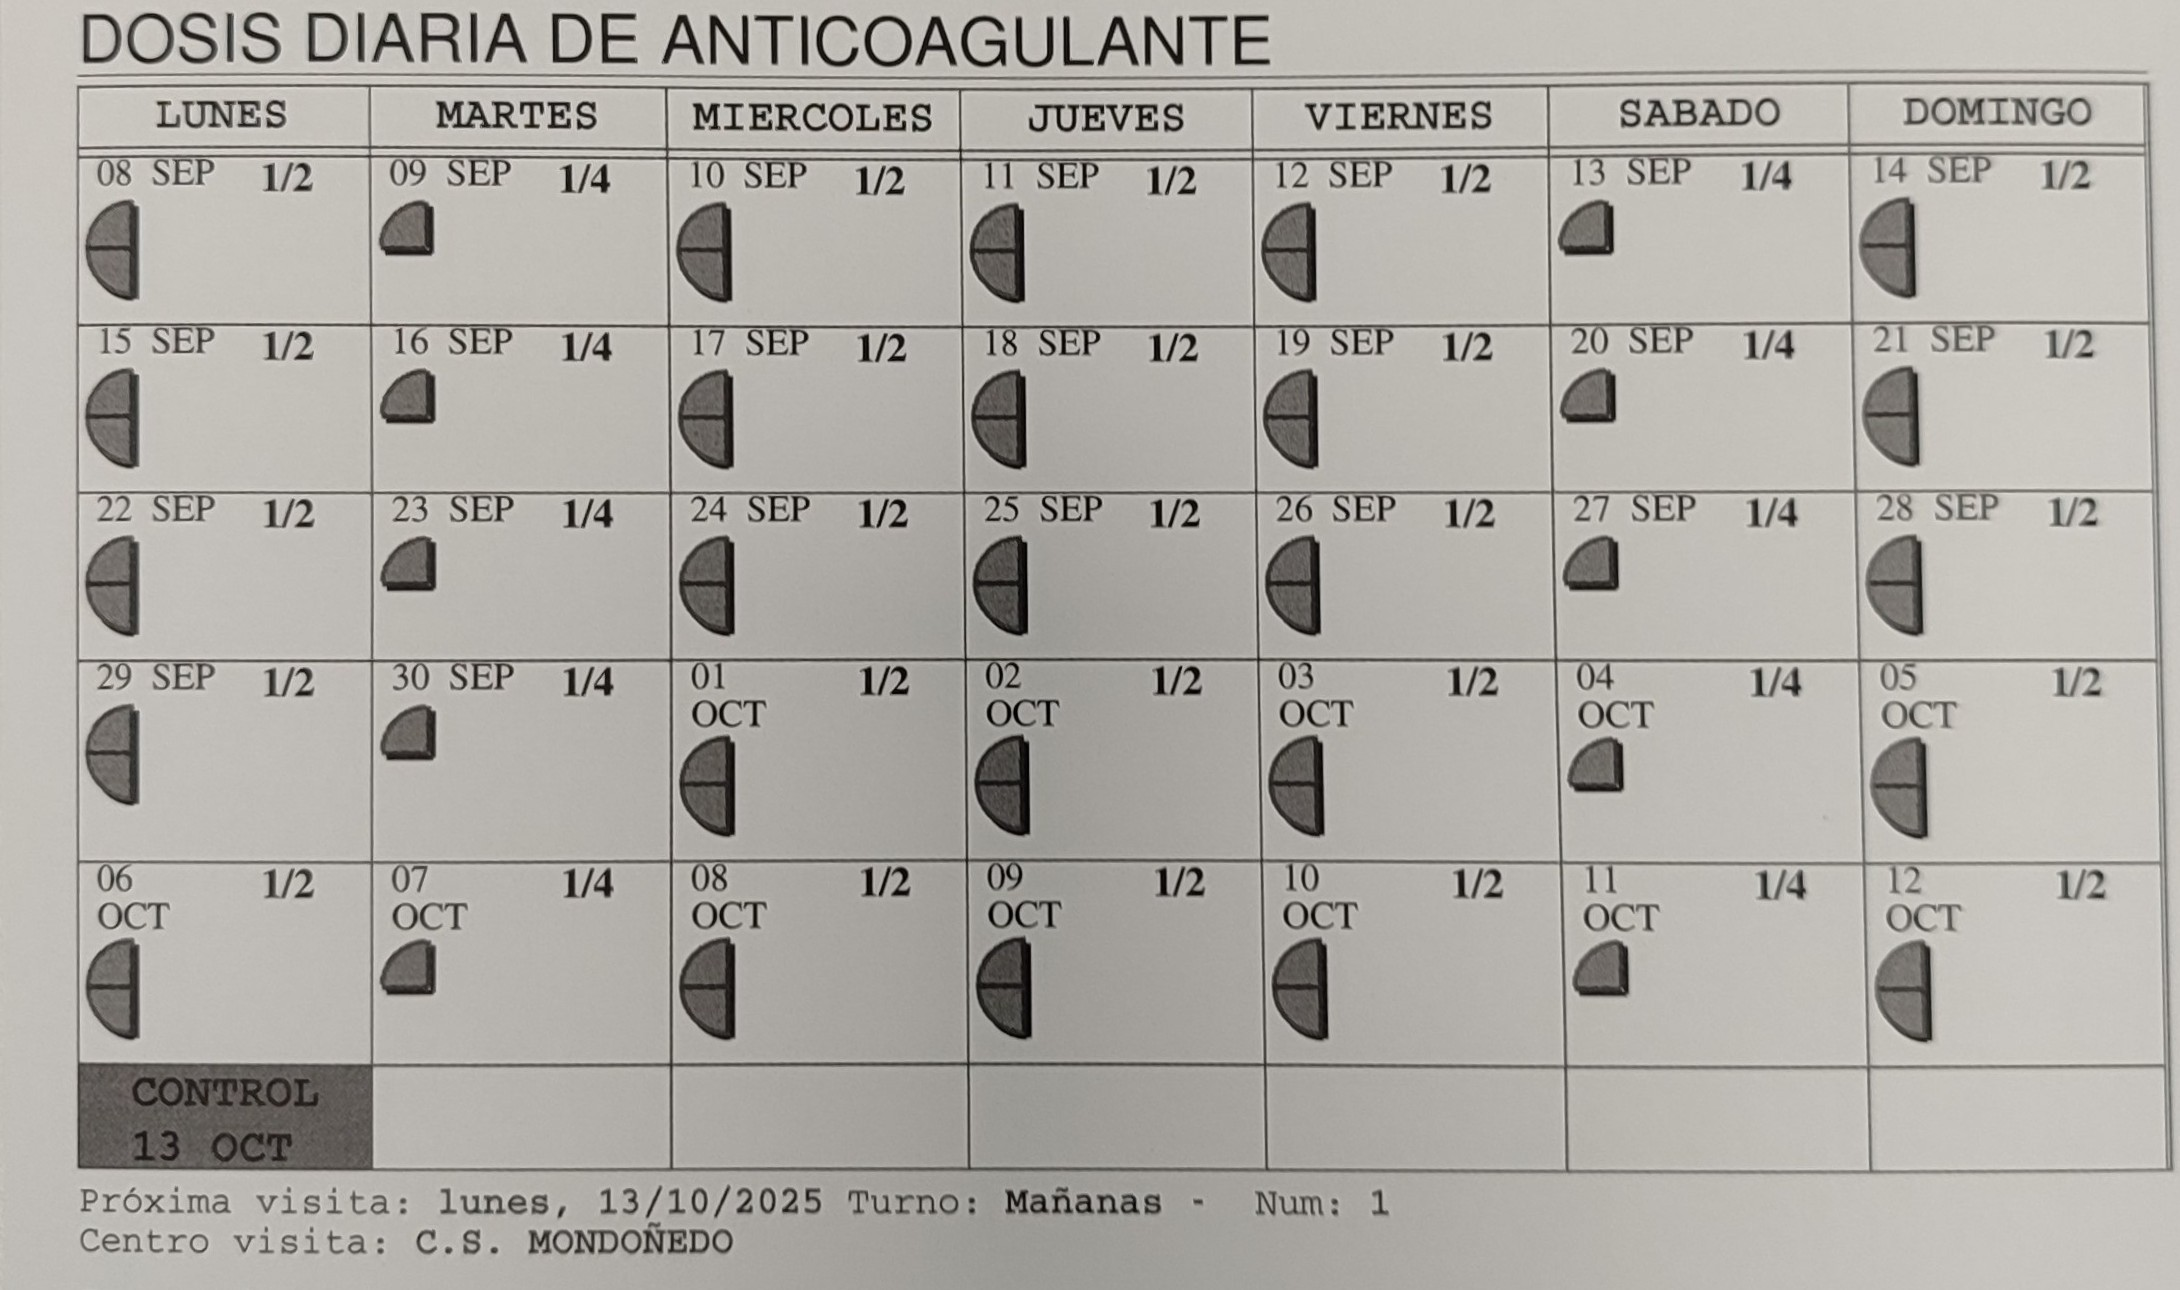
\includegraphics[width=0.65\textwidth]{imaxes/06-Procesamento automático das follas de tratamento/mlkit-f01n-pauta.jpg}
    \caption{Fragmento dunha folla escaneada empregada na avaliación do
    modelo estándar de Tesseract.}
    \label{fig:tesseract-estandar-f01}
\end{figure}

\begin{lstlisting}[
    frame=single,
    rulecolor=\color{gray!60},
    backgroundcolor=\color{gray!5},
    basicstyle=\ttfamily\scriptsize,
    caption={Fragmento da saída do modelo estándar de Tesseract para unha das follas escaneadas},
    label={lst:tesseract-estandar-f04},
    captionpos=t,
    columns=fullflexible,
    keepspaces=true
]
LUNES MARTES MIERCOLES JUEVES VIERNES SABADO |] DOMINGO
07 o [0 14 70 vo 10 va [1 o Ta
ENE ENE ENE ENE ENE
NO TOMAR a NO TOMAR NO TOMAR a
13 1/4 14 0 15 1/4
ENE ENE ENE
NO TOMAR
\end{lstlisting}

Noutros documentos o resultado foi aínda máis limitado. Na folla F02, por exemplo, Tesseract recoñeceu o título \textit{DOSIS DIARIA DE
ANTICOAGULANTE}, pero non recuperou o contido da táboa situada a continuación, pasando directamente á información da próxima visita.
Isto impide obter calquera asociación entre datas e doses para esa folla.

Os resultados non foron igualmente negativos en todos os documentos. Por exemplo, nalgunhas follas curtas Tesseract conseguiu conservar boa parte dunha fila da pauta. Porén, esta variabilidade entre documentos impide asumir que a mesma estratexia vaia proporcionar unha saída fiable para o conxunto de follas de tratamento.

Dado que estas limitacións apareceron xa nas follas escaneadas, non se considerou necesario estender a avaliación do modelo estándar a fotografías tomadas en diferentes condicións de captura. Os erros observados nas condicións máis favorables resultaban suficientes para descartar este modelo como solución directa. Estes resultados motivaron a realización de probas cun modelo de Tesseract adestrado especificamente para este tipo de documentos.

\subsubsection{Modelo personalizado}

O adestramento do modelo \textit{sintromv2} mostrou unha redución progresiva da taxa de erro ao longo do proceso. Como se observa na
Figura~\ref{fig:tesseract-sintromv2-adestramento}, o BCER pasou de valores próximos ao 39\,\% nas primeiras iteracións ata alcanzar un mínimo do \textbf{10,878\,\%}.

\begin{figure}[htbp]
    \centering
    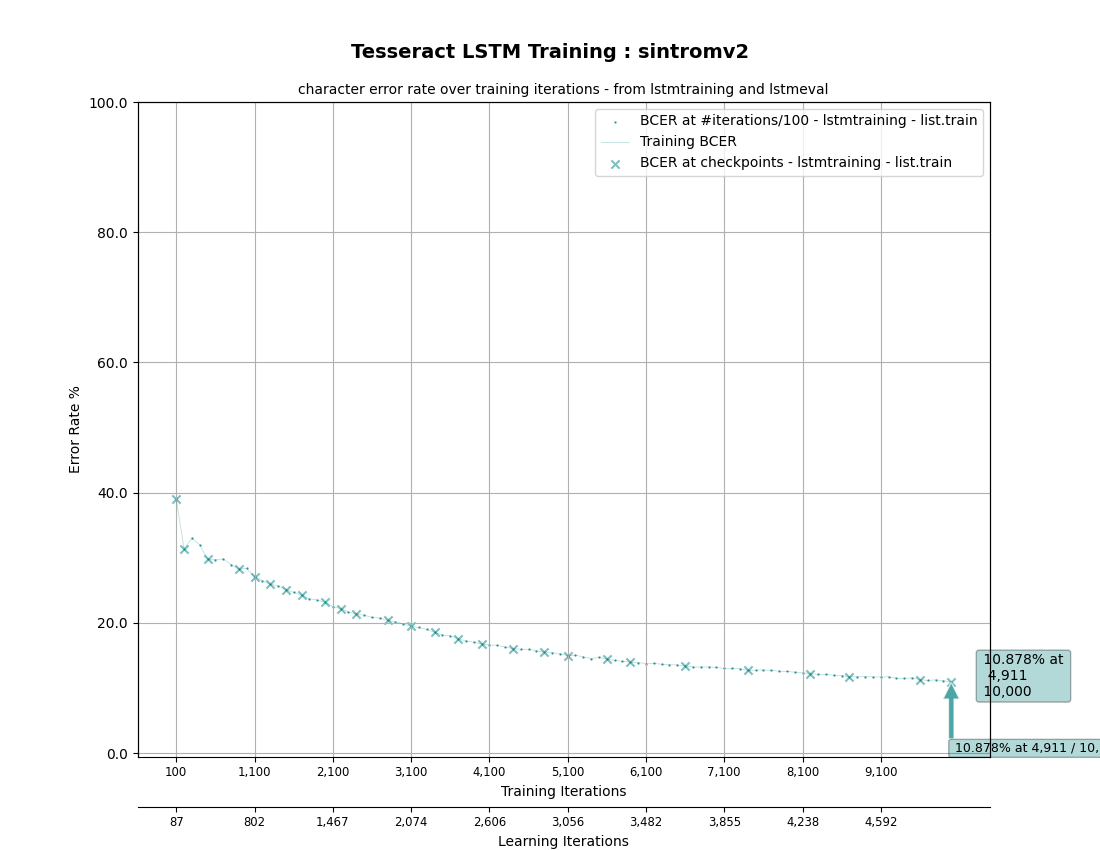
\includegraphics[width=0.75\textwidth]
    {imaxes/06-Procesamento automático das follas de tratamento/sintromv2.plot_cer.png}
    \caption{Evolución do BCER durante o adestramento do modelo
    \textit{sintromv2}.}
    \label{fig:tesseract-sintromv2-adestramento}
\end{figure}

O proceso completou as \textbf{10\,000 iteracións} empregadas por defecto por \textit{tesstrain} e obtivo o mellor resultado na
\textbf{iteración 4\,911}, cun BCER do \textbf{10,878\,\%} e un BWER do \textbf{20,409\,\%}. O punto de control correspondente a este resultado foi empregado para xerar o modelo final \textit{sintromv2}.

Seguindo a distribución indicada anteriormente, a avaliación realizouse sobre as follas \textbf{F09, F10 e F11}, que non foran empregadas durante o adestramento. As tres procesáronse nas catro condicións de captura definidas: imaxe escaneada, iluminación normal, menor iluminación e maior distancia.

Nas imaxes escaneadas observouse unha mellora respecto ao modelo estándar, especialmente no recoñecemento das fraccións empregadas para representar as doses. Un exemplo pode verse na folla F11, mostrada na  Figura~\ref{fig:tesseract-comparacion-f11}.

\begin{figure}[htbp]
\centering

\begin{minipage}[t]{0.48\textwidth}
\centering
\textbf{Modelo estándar}

\begin{lstlisting}[
    frame=single,
    rulecolor=\color{gray!60},
    backgroundcolor=\color{gray!5},
    basicstyle=\ttfamily\tiny,
    escapeinside={(*}{*)},
    columns=fullflexible,
    keepspaces=true
]
27 (*\textcolor{red}{12}*) 28 (*\textcolor{red}{12}*) 29 (*\textcolor{red}{12}*)
30 1/2 31 1/2 01 1/4
MAR MAR MAR MAR MAR ABR

02 (*\textcolor{red}{12}*) 03 (*\textcolor{red}{12}*) 04 (*\textcolor{red}{12}*)
ABR ABR ABR
\end{lstlisting}

\end{minipage}
\hfill
\begin{minipage}[t]{0.48\textwidth}
\centering
\textbf{Modelo \textit{sintromv2}}

\begin{lstlisting}[
    frame=single,
    rulecolor=\color{gray!60},
    backgroundcolor=\color{gray!5},
    basicstyle=\ttfamily\tiny,
    escapeinside={(*}{*)},
    columns=fullflexible,
    keepspaces=true
]
27 (*\textcolor{red}{1/2}*) 28 (*\textcolor{red}{1/2}*) 29 (*\textcolor{red}{1/2}*)
30 1/2 31 1/2 01 1/4
MAR MAR MAR MAR MAR ABR

02 (*\textcolor{red}{1/2}*) 03 (*\textcolor{red}{1/2}*) 04 (*\textcolor{red}{1/2}*)
ABR ABR ABR
\end{lstlisting}

\end{minipage}

\caption{Comparación dun fragmento da folla F11 co modelo estándar e co
modelo personalizado de Tesseract. En vermello destácanse algunhas das
fraccións corrixidas polo modelo \textit{sintromv2}.}
\label{fig:tesseract-comparacion-f11}
\end{figure}

A mellora non eliminou, con todo, os problemas de recoñecemento. Nas follas F09 e F10 continuaron aparecendo modificacións nas datas e perda da estrutura da táboa. Por exemplo, en F10 obtivéronse valores como \textit{068/09/2025} en lugar de \textit{08/09/2025} ou \textit{13/10/2023} en lugar de \textit{13/10/2025}, ao mesmo tempo que os elementos da pauta aparecían parcialmente desordenados.

Ao empregar fotografías, o comportamento empeorou. Mesmo con iluminación normal producíronse perdas importantes na táboa de doses; por exemplo, nunha das capturas de F10 recoñeceuse correctamente boa parte do texto xeral e a dose semanal, pero da pauta diaria practicamente só se conservaron os encabezados \textit{VIERNES} e \textit{DOMINGO}. Nas fotografías con menor iluminación e nas tomadas desde unha maior distancia a degradación foi aínda maior, chegando a obterse saídas nas que gran parte do texto e da estrutura do documento resultaban inintelixibles.

En conxunto, o adestramento específico permitiu mellorar o recoñecemento de determinados elementos, especialmente das fraccións. Porén, seguiron producíndose erros nas datas, nas doses e na organización da táboa, que se fixeron máis acusados ao empeorar as condicións de captura. Estes resultados impedían garantir unha reconstrución suficientemente fiable da pauta, polo que Tesseract foi descartado como solución principal para a extracción automática.

\subsection{Resultados de Azure AI Document Intelligence}

A avaliación de Azure AI Document Intelligence realizouse comparando os dous modelos personalizados adestrados, \textit{Template} e \textit{Neural}. Primeiro analizáronse as métricas proporcionadas ao finalizar o adestramento e, posteriormente, avaliáronse ambos modelos sobre as follas reservadas para as probas.

No modelo \textit{Template}, mostrado na Figura~\ref{fig:azure-metricas-template}, Azure proporciona unha estimación da precisión para cada un dos campos definidos.Os valores foron elevados na maior parte dos campos: 99,50\,\% para \textit{fecha visita}, \textit{inr}, \textit{farmaco oral} e \textit{prox visit}, 98,80\,\% para \textit{DOSE} e 94,70\,\% para \textit{RUV}. Os valores máis baixos corresponden a \textit{dosis semanal} e \textit{centro visita}, cun 87,50\,\%, e a \textit{turno}, cun 62,50\,\%. . Non obstante, estes campos teñen unha relevancia secundaria dentro da aplicación, xa que non afectan ao procesamento principal. En consecuencia, aínda que estes resultados son inferiores aos do resto dos campos, non representan un impacto significativo sobre o rendemento global do sistema.

%Bibliografía de azure  e poñer unha nota ou algo
No modelo \textit{Neural}, Azure Document Intelligence non proporciona puntuacións de precisión por campo durante o adestramento, polo que estes valores aparecen sen informar no Studio. Isto responde ao propio funcionamento deste tipo de modelo e non indica un erro no proceso de adestramento.

\begin{figure}[htbp]
    \centering
    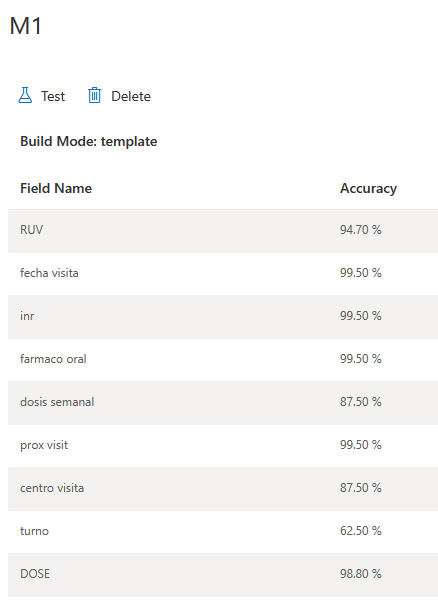
\includegraphics[width=0.4\textwidth]
    {imaxes/06-Procesamento automático das follas de tratamento/ResultM1.png}
    \caption{Precisión por campo mostrada por Azure Document Intelligence
    Studio para o modelo \textit{Template}.}
    \label{fig:azure-metricas-template}
\end{figure}


Nas probas sobre documentos non vistos, ambos modelos conseguiron recuperar correctamente numerosos campos individuais, como o INR, fármaco oral ou a data da visita. A principal diferenza apareceu na extracción da pauta diaria. O modelo \textit{Template} conservou de forma moito máis estable a agrupación dos días e das doses dentro das filas da táboa, mentres que o modelo \textit{Neural} fragmentou con frecuencia estes elementos en rexistros separados.

A plataforma de Azure devolve a información extraída nun documento con formato JSON para que poida ser consumido. O problema subxacente desta mala lectura visual é que o JSON resultante herda todo este caos. Ao non seguir un patrón predicible na súa resposta (nalgúns casos o JSON devolve a data e a dose xuntas, noutros devólveas separadas en distintas filas do obxecto …), resulta practicamente imposible deseñar unha lóxica de extracción que sexa capaz de recoller a información correcta para o día adecuado de forma robusta e automática

Un exemplo representativo desta diferenza pode observarse na folla F10 con iluminación normal. Como se mostra na Figura~\ref{fig:azure-comparacion-f10n}, o modelo \textit{Template} mantén nun mesmo rexistro os valores correspondentes aos sete días da semana. No modelo \textit{Neural}, pola contra, parte das datas e das doses son separadas en rexistros diferentes. Por exemplo, \textit{14 OCT} aparece separado da súa dose \textit{1/4}, dificultando a reconstrución directa da relación entre ambos elementos.

% Primeiro bloque (Páxina 1)
\begin{figure}[htbp]
    \centering
    
    % Primeira imaxe: Aumentamos o tamaño ao 90% do ancho do texto (\textwidth)
    \begin{subfigure}[t]{0.9\textwidth}
        \centering
        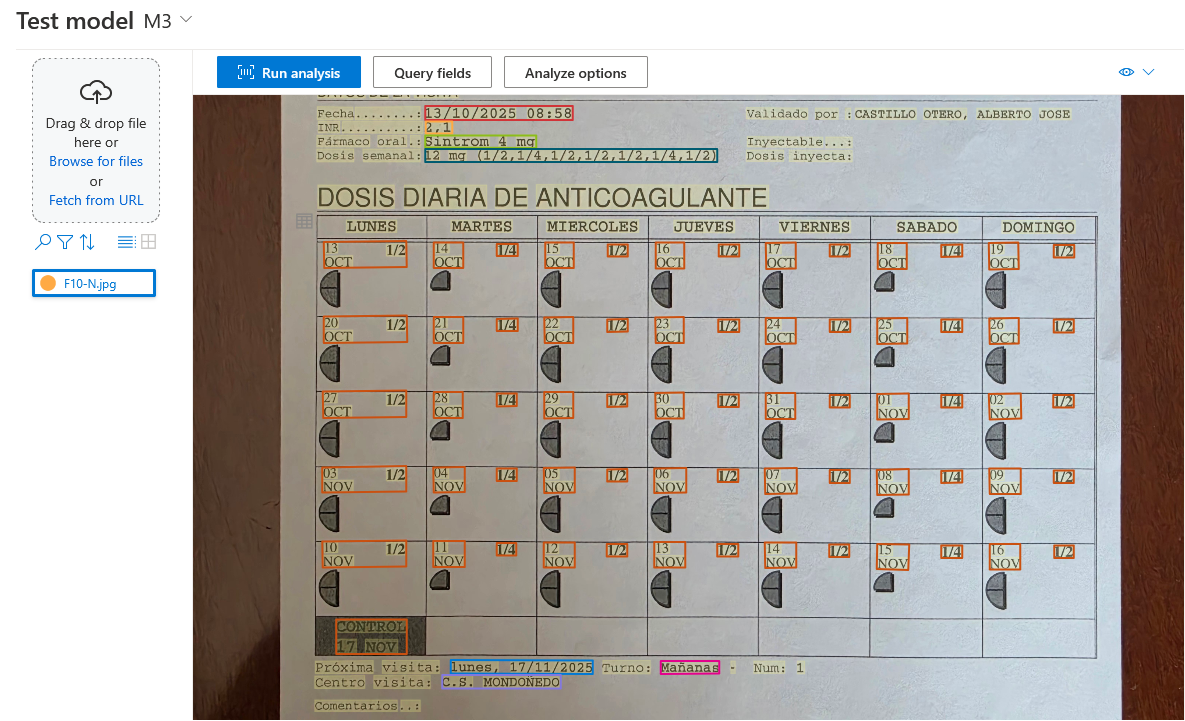
\includegraphics[width=\linewidth]{imaxes/06-Procesamento automático das follas de tratamento/azure-f10n-neural.png}
        \caption{Modelo \textit{Neural}.}
    \end{subfigure}
    
    \vspace{0.5cm} % Engadimos espazo vertical en lugar de \hfill
    
    % Segunda imaxe
    \begin{subfigure}[t]{0.9\textwidth}
        \centering
        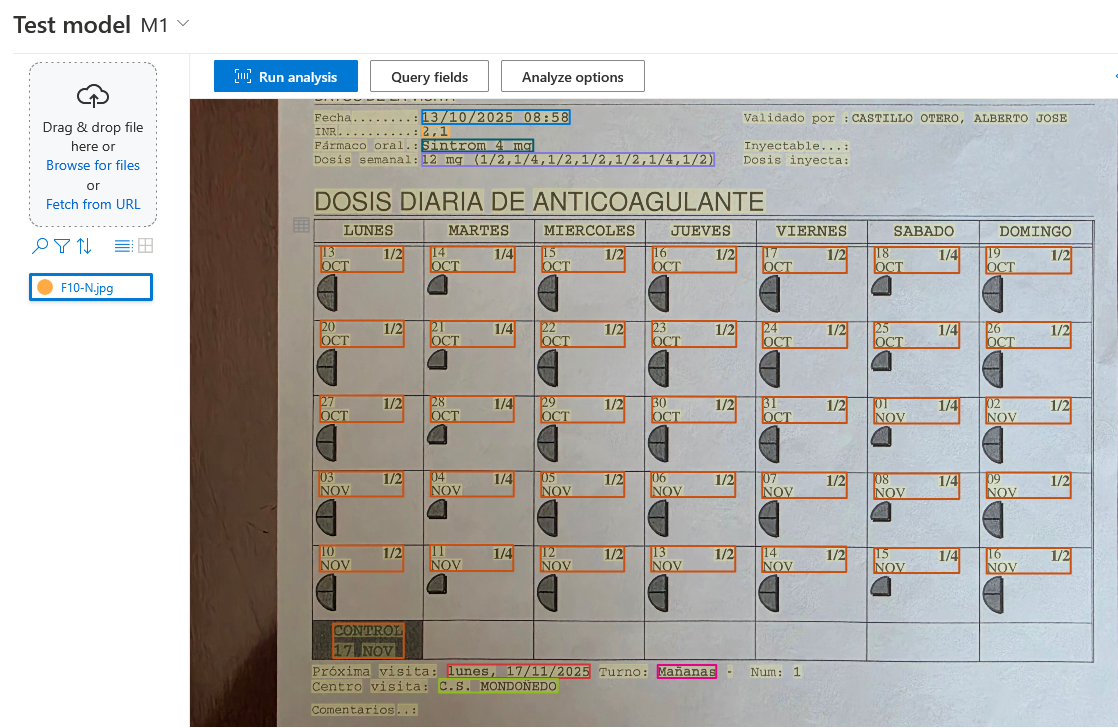
\includegraphics[width=\linewidth]{imaxes/06-Procesamento automático das follas de tratamento/azure-f10n-template.png}
        \caption{Modelo \textit{Template}.}
    \end{subfigure}

    \caption{Comparación da extracción da pauta da folla F10 con iluminación normal mediante os modelos \textit{Neural} e \textit{Template} (Parte 1).}
    \label{fig:azure-comparacion-f10n-1}
\end{figure}

% Segundo bloque (Páxina 2 ou a seguinte dispoñible)
\begin{figure}[htbp]
    \ContinuedFloat % <--- ISTO É A CLAVE: Dille a LaTeX que é a mesma figura que a anterior
    \centering
    
    % Terceira imaxe
    \begin{subfigure}[t]{0.9\textwidth}
        \centering
        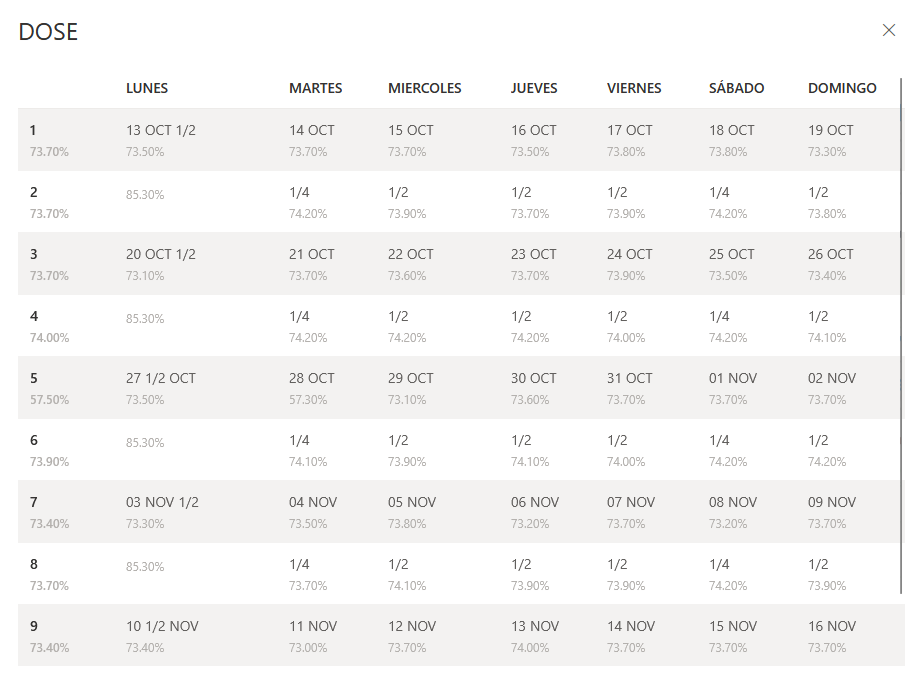
\includegraphics[width=\linewidth]{imaxes/06-Procesamento automático das follas de tratamento/azure-f10n-neural-taboa.png}
        \caption{Modelo \textit{Neural} (Táboas).}
    \end{subfigure}
    
    \vspace{0.5cm}
    
    % Cuarta imaxe
    \begin{subfigure}[t]{0.9\textwidth}
        \centering
        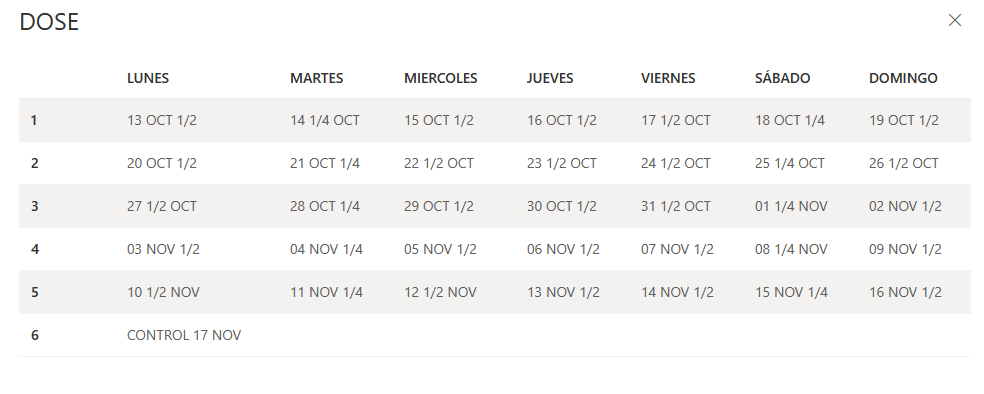
\includegraphics[width=\linewidth]{imaxes/06-Procesamento automático das follas de tratamento/azure-f10n-template-taboa.png}
        \caption{Modelo \textit{Template} (Táboas).}
    \end{subfigure}

    \caption{Comparación da extracción da pauta da folla F10 con iluminación normal mediante os modelos \textit{Neural} e \textit{Template} (Continuación).}
    \label{fig:azure-comparacion-f10n} % Esta é a etiqueta xeral que debes usar para referenciala no texto
\end{figure}

O modelo \textit{Template} non estivo exento de erros. Por exemplo, na folla F09 o campo \textit{turno} foi asociado incorrectamente co valor \textit{C.S. MONDOÑEDO}, mentres que o modelo \textit{Neural} recuperou correctamente \textit{Mañanas}.  Este resultado é coherente coa menor precisión obtida por este campo durante o adestramento do modelo \textit{Template}.


Nas condicións con menor iluminación, a cela de control resultou máis difícil de extraer correctamente debido ao sombreado escuro da propia cela, sobre o que se representan caracteres tamén escuros. Por exemplo, a entrada \textit{CONTROL 05 ABR} foi devolta unicamente como \textit{CONTROL}, perdéndose a data asociada.Esta perda non supón unha limitación práctica para
a aplicación, xa que a data do seguinte control pode obterse tamén a partir do campo \textit{prox visit}. Este campo presentou unha precisión do 99,50\,\% no modelo \textit{Template} e foi extraído correctamente en todas as probas realizadas.

En conxunto, ambos modelos permitiron recuperar unha parte importante da información das follas e mostraron un bo comportamento nos campos individuais. As principais diferenzas apareceron na estrutura da pauta diaria, onde o modelo \textit{Template} conservou de maneira máis consistente a asociación entre cada data e a súa dose. Aínda que se detectaron erros puntuais,
especialmente nas condicións de captura menos favorables, os resultados obtidos favoreceron este modelo para o procesamento estruturado das follas.



 \chapter{Deseño}
\label{chap:deseño}

Neste capítulo descríbese o deseño da solución, incluíndo a arquitectura do sistema, o modelo de información e de persistencia, os principais fluxos de interacción e a navegación da interface. O obxectivo é presentar as decisións que determinan a organización e o comportamento da aplicación, mentres que a súa materialización no código se explica no Capítulo~\ref{chap:implem}. Os diagramas e fluxos complementarios recóllense no Apéndice~\ref{app:deseno-detallado}.

\section{Arquitectura da solución}

\subsection{Visión xeral do sistema}

A solución segue unha \textbf{arquitectura cliente-servidor} formada por unha aplicación móbil e unha \gls{api} baseada no estilo \gls{rest}. O cliente constitúe o punto de interacción coa persoa usuaria e encárgase do seguimento do tratamento, a persistencia local e as notificacións. A \gls{api} centraliza o procesamento das follas, aplica as regras necesarias para reconstruír a pauta e proporciona acceso aos servizos externos empregados pola solución.

Esta separación evita incorporar no cliente as credenciais e a lóxica de acceso ao servizo de procesamento documental. Ademais, permite modificar ou substituír ese servizo sen alterar o fluxo empregado pola aplicación, sempre que se conserve o contrato de comunicación establecido.

A información clínica e o seguimento das tomas almacénanse localmente nos dispositivos. En consecuencia, a \gls{api} non mantén unha base de datos central cos tratamentos das persoas usuarias e cada petición contén a información necesaria para ser procesada. Esta decisión reduce a cantidade de datos sensibles conservados no servidor e permite consultar a pauta xa gardada sen depender continuamente dunha conexión de rede.

Outro criterio relevante foi non incorporar automaticamente os resultados da extracción ao tratamento activo. Debido a que o proceso documental pode producir datos incompletos ou incorrectos, a pauta pasa sempre por unha fase de revisión e validación antes de ser confirmada.

\subsection{Arquitectura do cliente móbil}

O cliente organízase seguindo o patrón \textit{Model-View-ViewModel} (MVVM). As \textbf{vistas} representan as pantallas e recollen as interaccións da persoa usuaria. Os \textbf{modelos de vista} manteñen o estado asociado ás distintas funcionalidades e coordinan as operacións necesarias. Pola súa parte, os \textbf{modelos} representan a información coa que traballa a aplicación.

A estas capas engádese un conxunto de \textbf{servizos} que encapsulan as operacións que non pertencen directamente á interface, como o acceso á \gls{api}, a persistencia, as notificacións, o almacenamento seguro ou a sincronización. Esta separación permite que as pantallas non necesiten coñecer como se executan esas operacións e facilita probar a lóxica dos modelos de vista de maneira illada.

Os compoñentes visuais reutilizables e os recursos compartidos mantéñense tamén separados das funcionalidades concretas. A correspondencia entre estas responsabilidades e a estrutura de paquetes do proxecto móstrase no Apéndice~\ref{app:deseno-detallado}.

\subsection{Arquitectura da API}

A \gls{api} deseñouse como un servizo sen estado: cada petición é independente e non require unha sesión almacenada no servidor. A súa organización separa catro responsabilidades principais:

\begin{itemize}
    \item os \textbf{puntos de entrada}, que reciben e verifican as peticións;
    \item a \textbf{lóxica interna}, que preprocesa, interpreta, transforma e valida os datos;
    \item os \textbf{esquemas}, que definen os contratos de entrada e saída;
    \item as \textbf{dependencias}, que proporcionan o acceso aos servizos externos.
\end{itemize}

Esta división evita mesturar a comunicación \gls{http} coa lóxica de procesamento e permite substituír as dependencias externas durante as probas. Os contratos \gls{rest} agrúpanse segundo a súa finalidade: extracción das follas, preprocesamento independente, consulta de centros sanitarios, comprobación do estado do servizo e reenvío de notificacións entre dispositivos vinculados.

A Figura~\ref{fig:arquitectura-mvvm-api} mostra conxuntamente a organización do cliente e da \gls{api}, así como a comunicación cos servizos externos.

\begin{figure}[htbp]
    \centering
    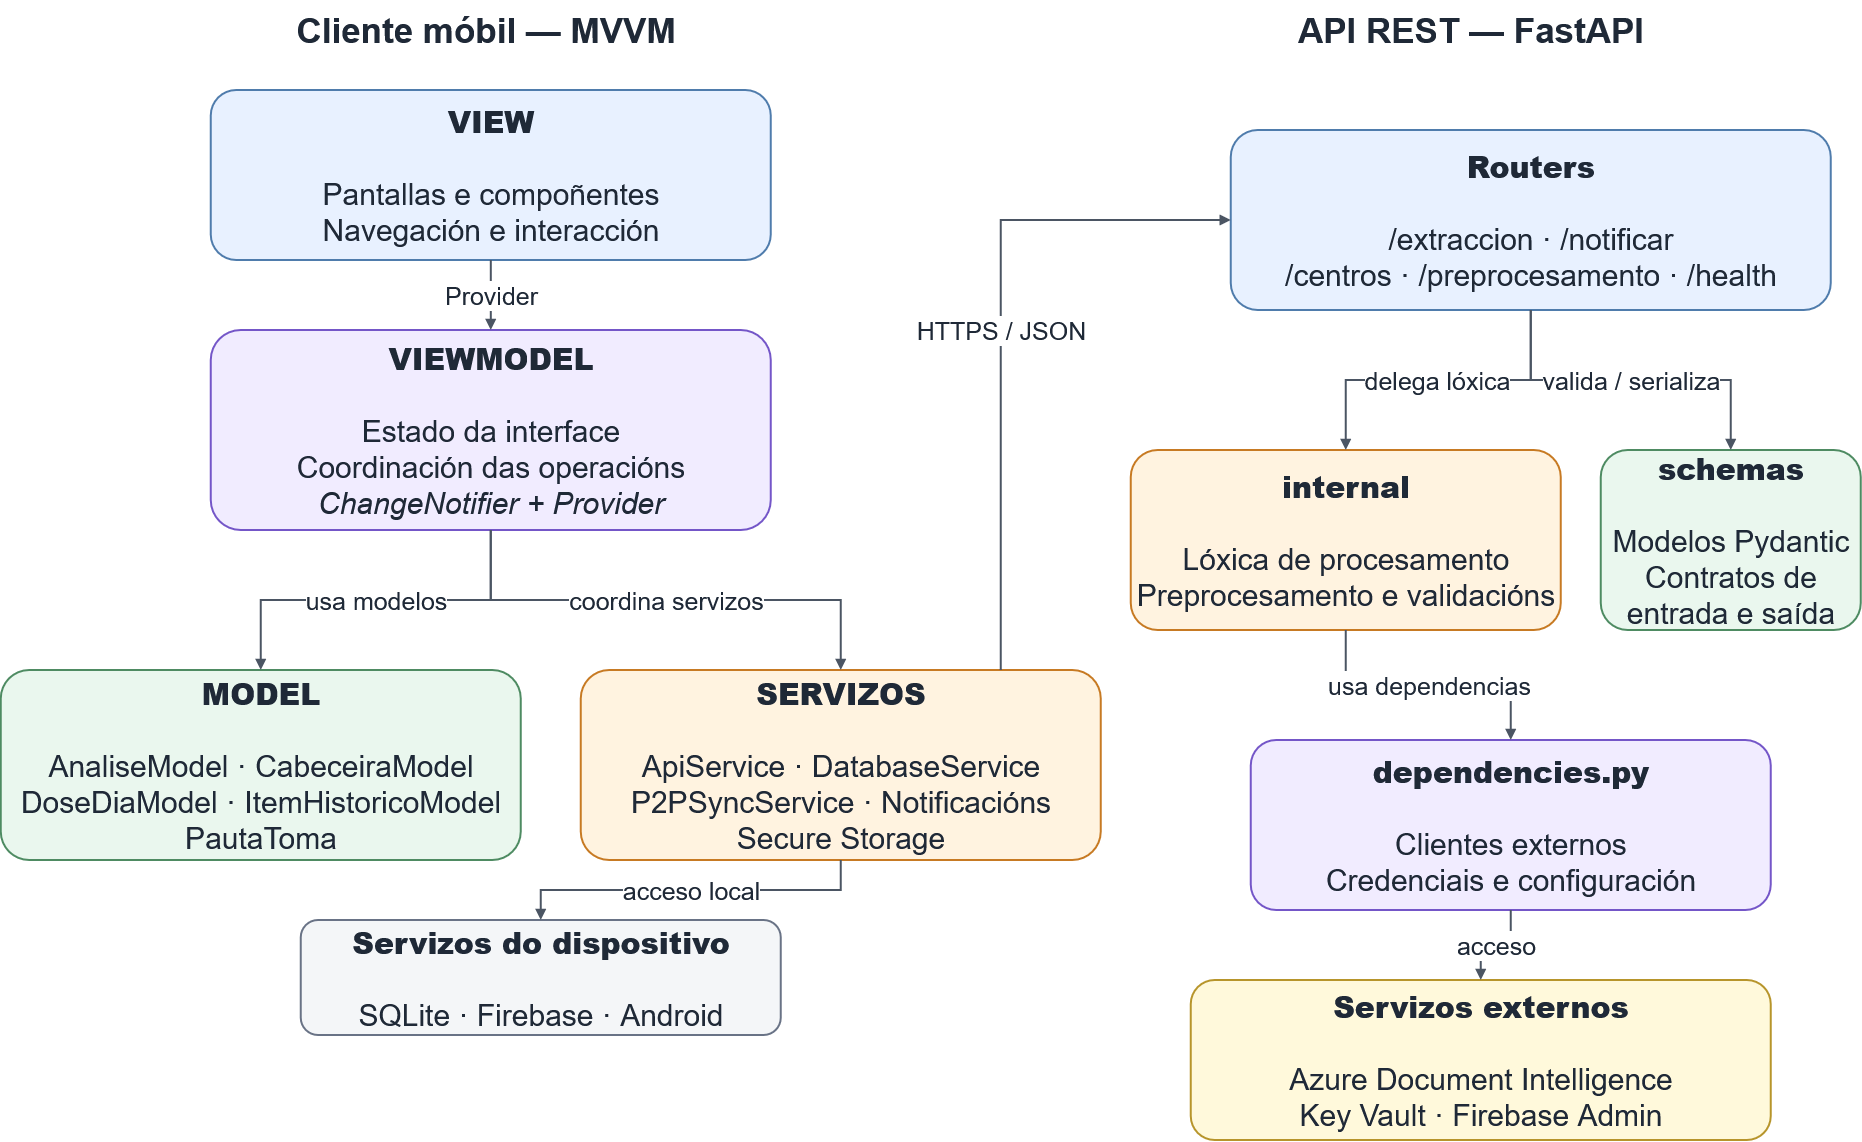
\includegraphics[width=0.92\textwidth]{imaxes/07-Deseño/02_cliente_mvvm_api.drawio(1).png}
    \caption{Arquitectura do cliente móbil e da API.}
    \label{fig:arquitectura-mvvm-api}
\end{figure}

\section{Modelo de información e persistencia}

\subsection{Modelo de información da aplicación}

O modelo principal representa os datos obtidos dunha folla de tratamento e a información necesaria para revisalos e realizar posteriormente o seguimento das tomas.

A entidade principal é a \textbf{análise}, que agrupa tres bloques: a cabeceira, a pauta diaria e o histórico de visitas. A cabeceira reúne datos xerais como a data do informe, o \gls{inr}, o fármaco, a dose semanal, a seguinte visita e o centro sanitario. A pauta diaria está formada polos días de tratamento e indica para cada un deles a data, a dose ou acción correspondente e se se trata dun día de control. O histórico conserva a información das visitas anteriores incluídas no documento.

Sobre esta análise actúa a \textbf{revisión da pauta}. Durante esta etapa poden corrixirse doses e datas, engadir ou eliminar días, modificar a seguinte visita, ordenar a pauta e comprobar a súa consistencia. Deste xeito, diferéncianse os datos propostos pola extracción automática dos datos que a persoa usuaria confirma finalmente.

Unha vez confirmada a pauta, cada dose pasa a formar parte do \textbf{seguimento das tomas}. Ademais da información prescrita, consérvase o estado de cada toma para distinguir se permanece pendente, foi realizada, foi realizada fóra da hora prevista ou non se realizou.

A Figura~\ref{fig:modelo-dominio} mostra os principais elementos deste modelo e as relacións entre eles.

\begin{figure}[htbp]
    \centering
    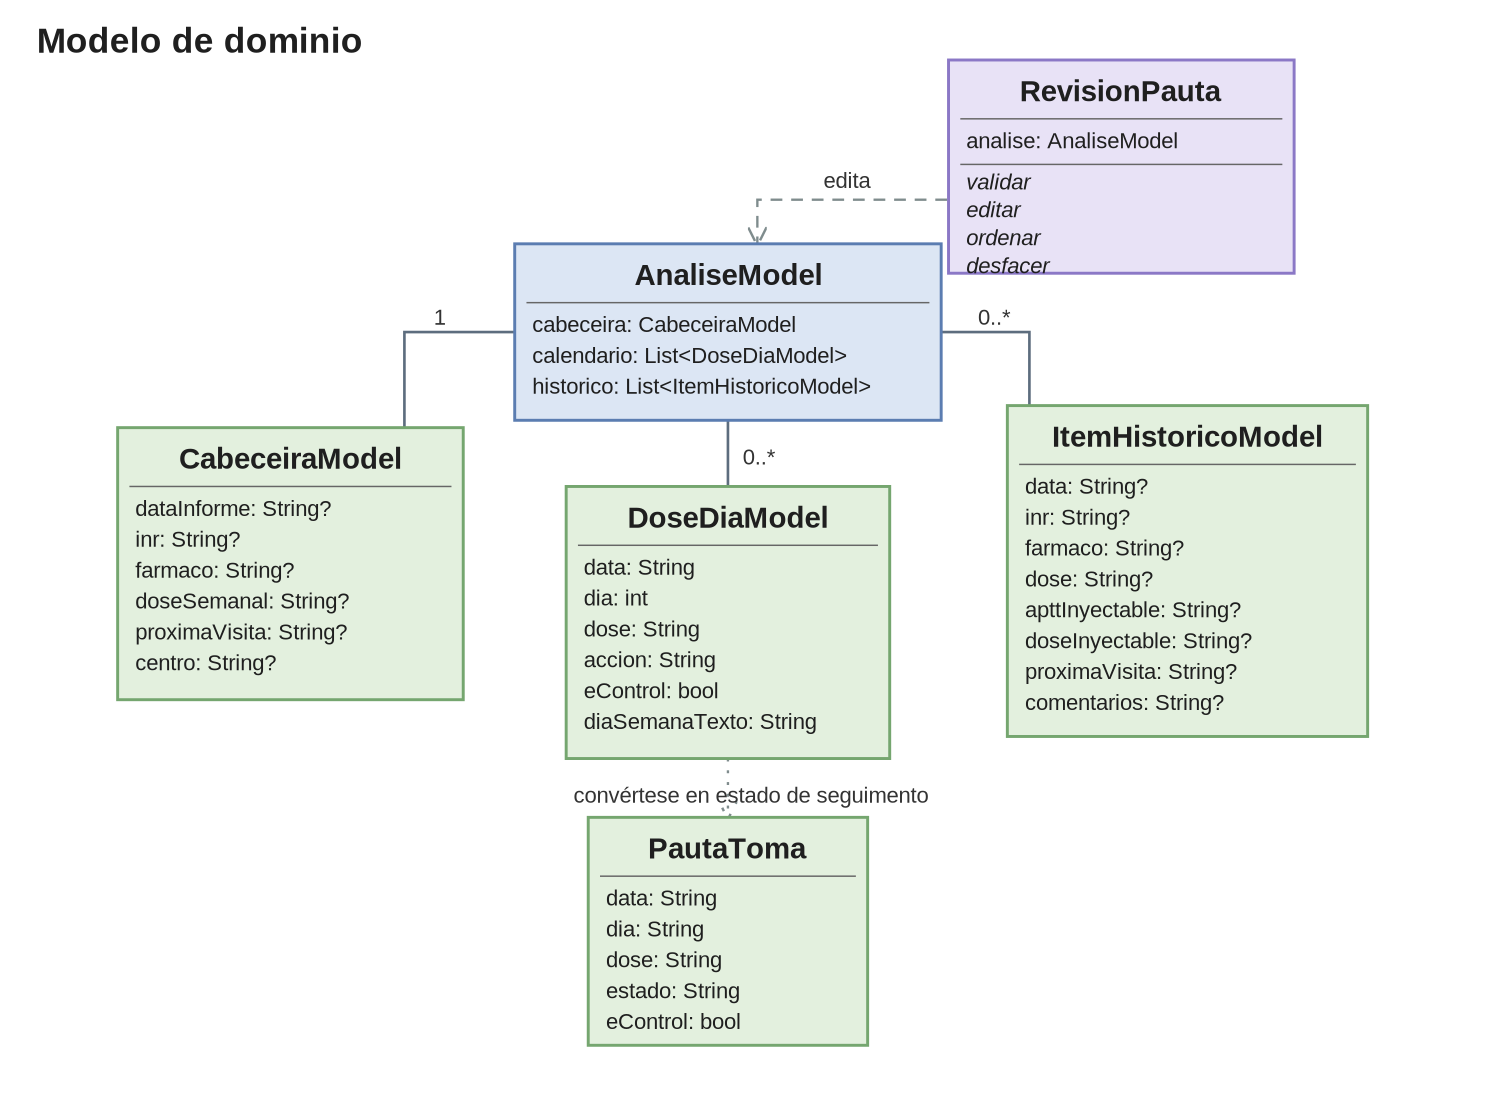
\includegraphics[width=0.8\textwidth]{imaxes/07-Deseño/modelo_dominio_uml_preview.png}
    \caption{Modelo principal de información da aplicación.}
    \label{fig:modelo-dominio}
\end{figure}

\subsection{Modelo de persistencia}

O almacenamento local organízase arredor da pauta vixente, o histórico de visitas e os datos necesarios para a supervisión. A \textbf{pauta vixente} reúne a última folla confirmada e o plan diario, incluíndo o estado das tomas. Cando se confirma unha nova folla, esta substitúe a pauta anterior, polo que só existe un tratamento activo en cada momento.

O \textbf{histórico de visitas} consérvase separado da pauta vixente para permitir consultar a evolución sen mesturala cos datos empregados no seguimento diario. Nos dispositivos das persoas supervisoras almacénanse tamén os \textbf{datos de supervisión}, formados polas persoas vinculadas e pola última información recibida de cada unha delas.

Finalmente, os \textbf{datos de configuración e seguridade}, como o rol, as preferencias e as claves asociadas ás vinculacións, mantéñense separados da base de datos clínica. As claves e os identificadores sensibles gárdanse mediante almacenamento seguro do sistema operativo.

\begin{figure}[htbp]
    \centering
    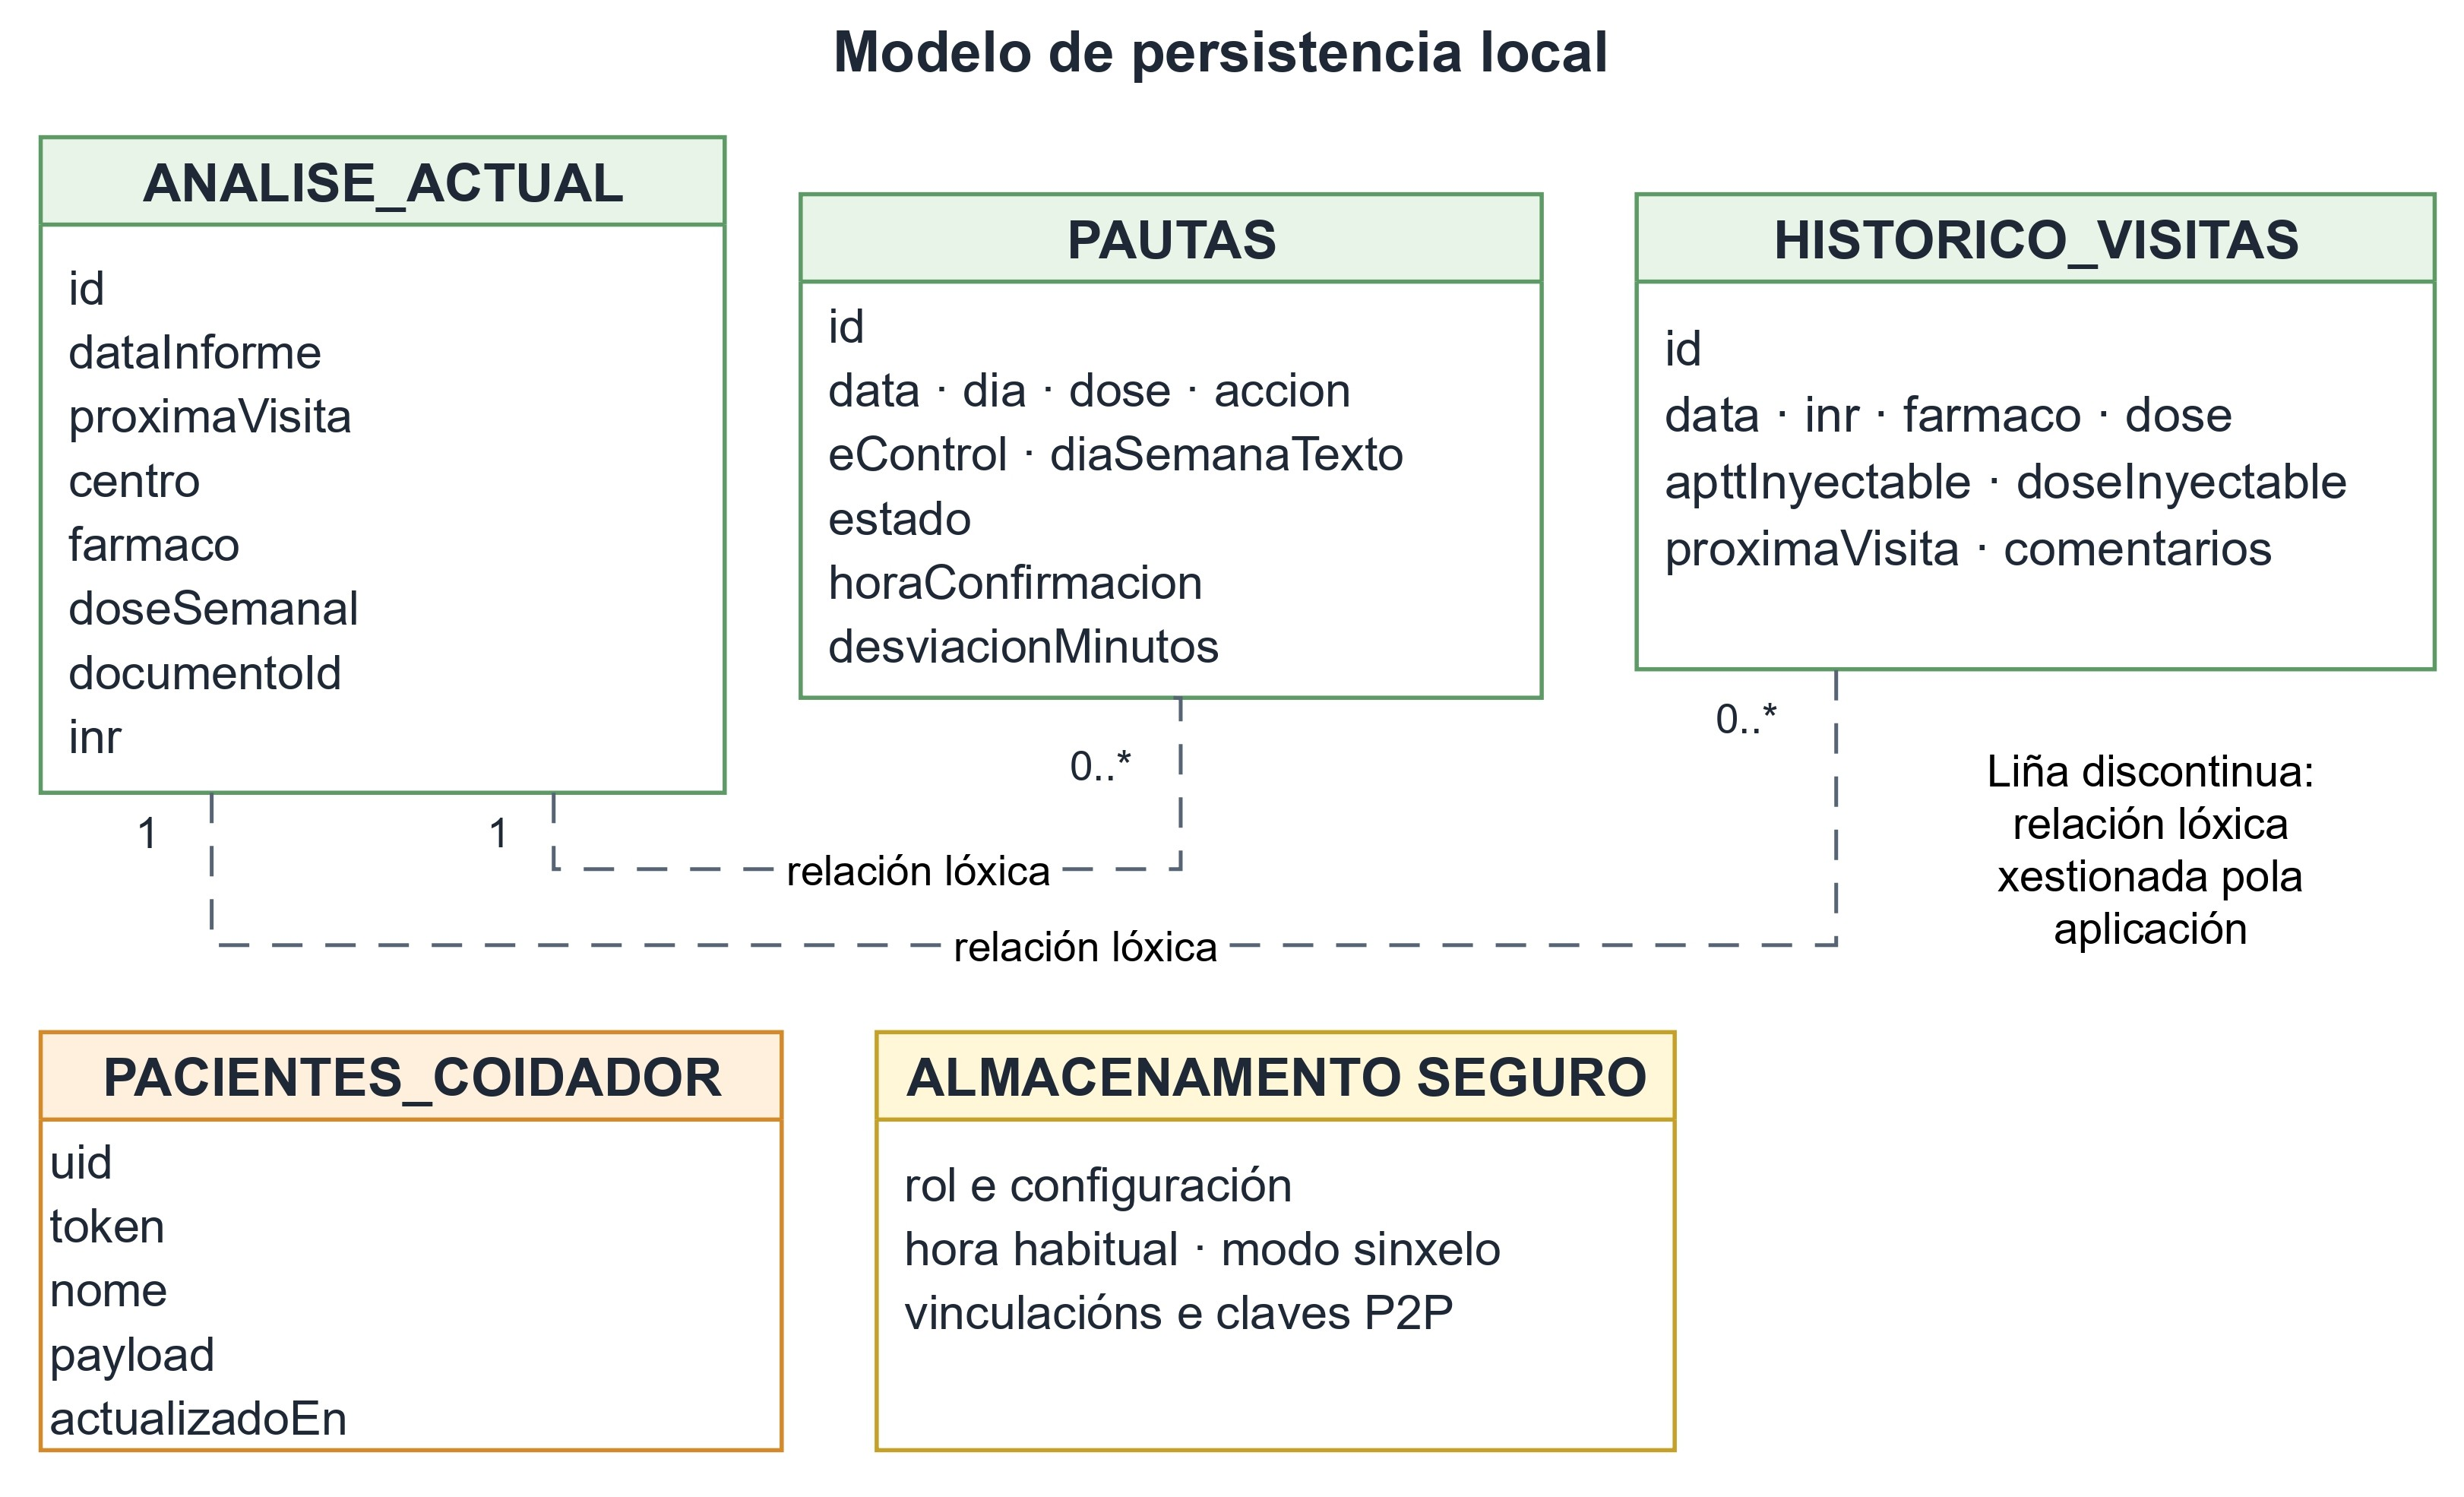
\includegraphics[width=0.8\textwidth]{imaxes/07-Deseño/modelo-persistencia_page-0001.jpg}
    \caption{Modelo entidade--relación da persistencia local.}
    \label{fig:modelo-persistencia}
\end{figure}

\section{Deseño do comportamento}

Nesta sección descríbense os tres fluxos que conectan máis compoñentes da solución: a vinculación entre os dispositivos, o procesamento dunha folla e a sincronización do tratamento.

\subsection{Vinculación entre paciente e supervisor}

A vinculación establécese mediante un código \gls{qr} xerado no dispositivo do paciente. Este código contén un identificador da vinculación, os datos necesarios para localizar o dispositivo e unha clave temporal empregada para protexer o intercambio inicial.

O supervisor escanea o código e utiliza estes datos para iniciar a asociación. Como resposta, envía a súa identificación xunto cunha nova clave compartida que se empregará nas comunicacións posteriores. A información transmítese cifrada coa clave temporal e, unha vez completado o intercambio, ambos os dispositivos dispoñen dos datos necesarios para identificarse e comunicarse de maneira segura.

\begin{figure}[htbp]
    \centering
    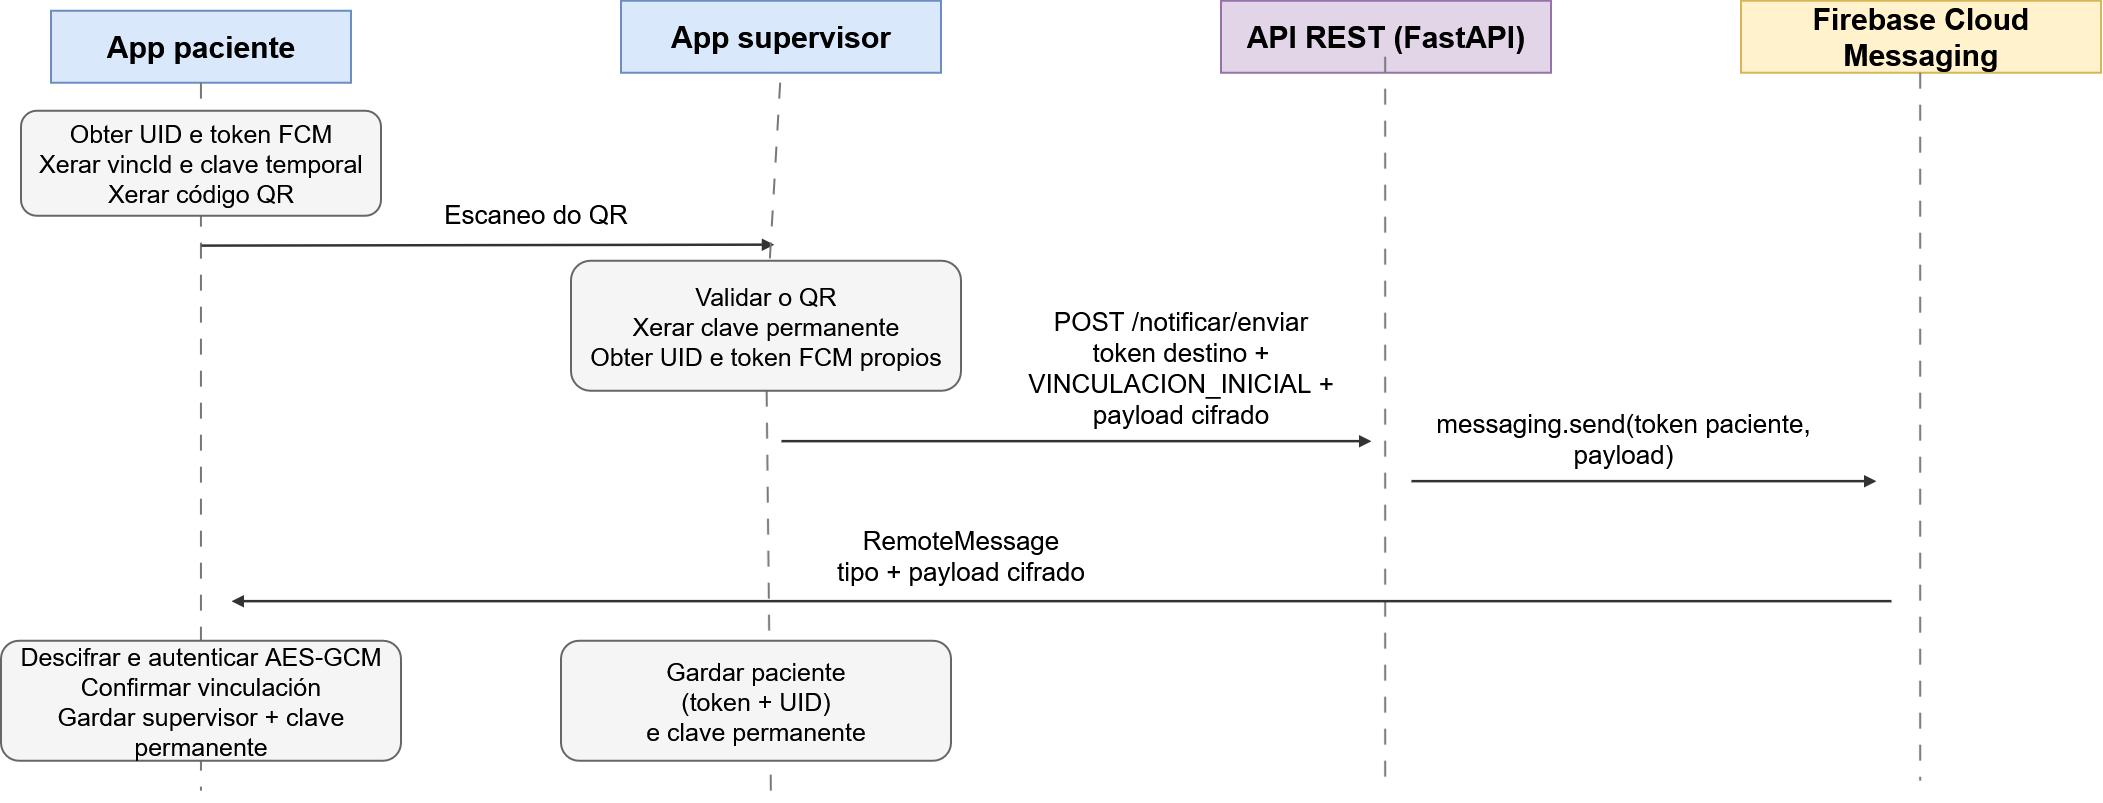
\includegraphics[width=0.9\textwidth]{imaxes/07-Deseño/secuencia_vinculacion_UML.drawio.png}
    \caption{Fluxo de vinculación entre paciente e supervisor.}
    \label{fig:fluxo-vinculacion}
\end{figure}

\subsection{Procesamento dunha folla de tratamento}

O fluxo comeza cando a persoa usuaria selecciona ou captura unha folla desde a aplicación. O documento envíase á \gls{api}, que comproba o formato, realiza o preprocesamento cando é necesario e solicita a extracción ao servizo documental.

A partir do resultado, a \gls{api} normaliza os campos, reconstrúe a pauta diaria e realiza as validacións definidas antes de devolver unha resposta. No cliente, os datos móstranse nunha pantalla de revisión e só pasan a formar parte da pauta activa despois da confirmación. Se a extracción non supera as comprobacións mínimas, o fluxo interrómpese e solicítase unha nova captura.

\begin{figure}[htbp]
    \centering
    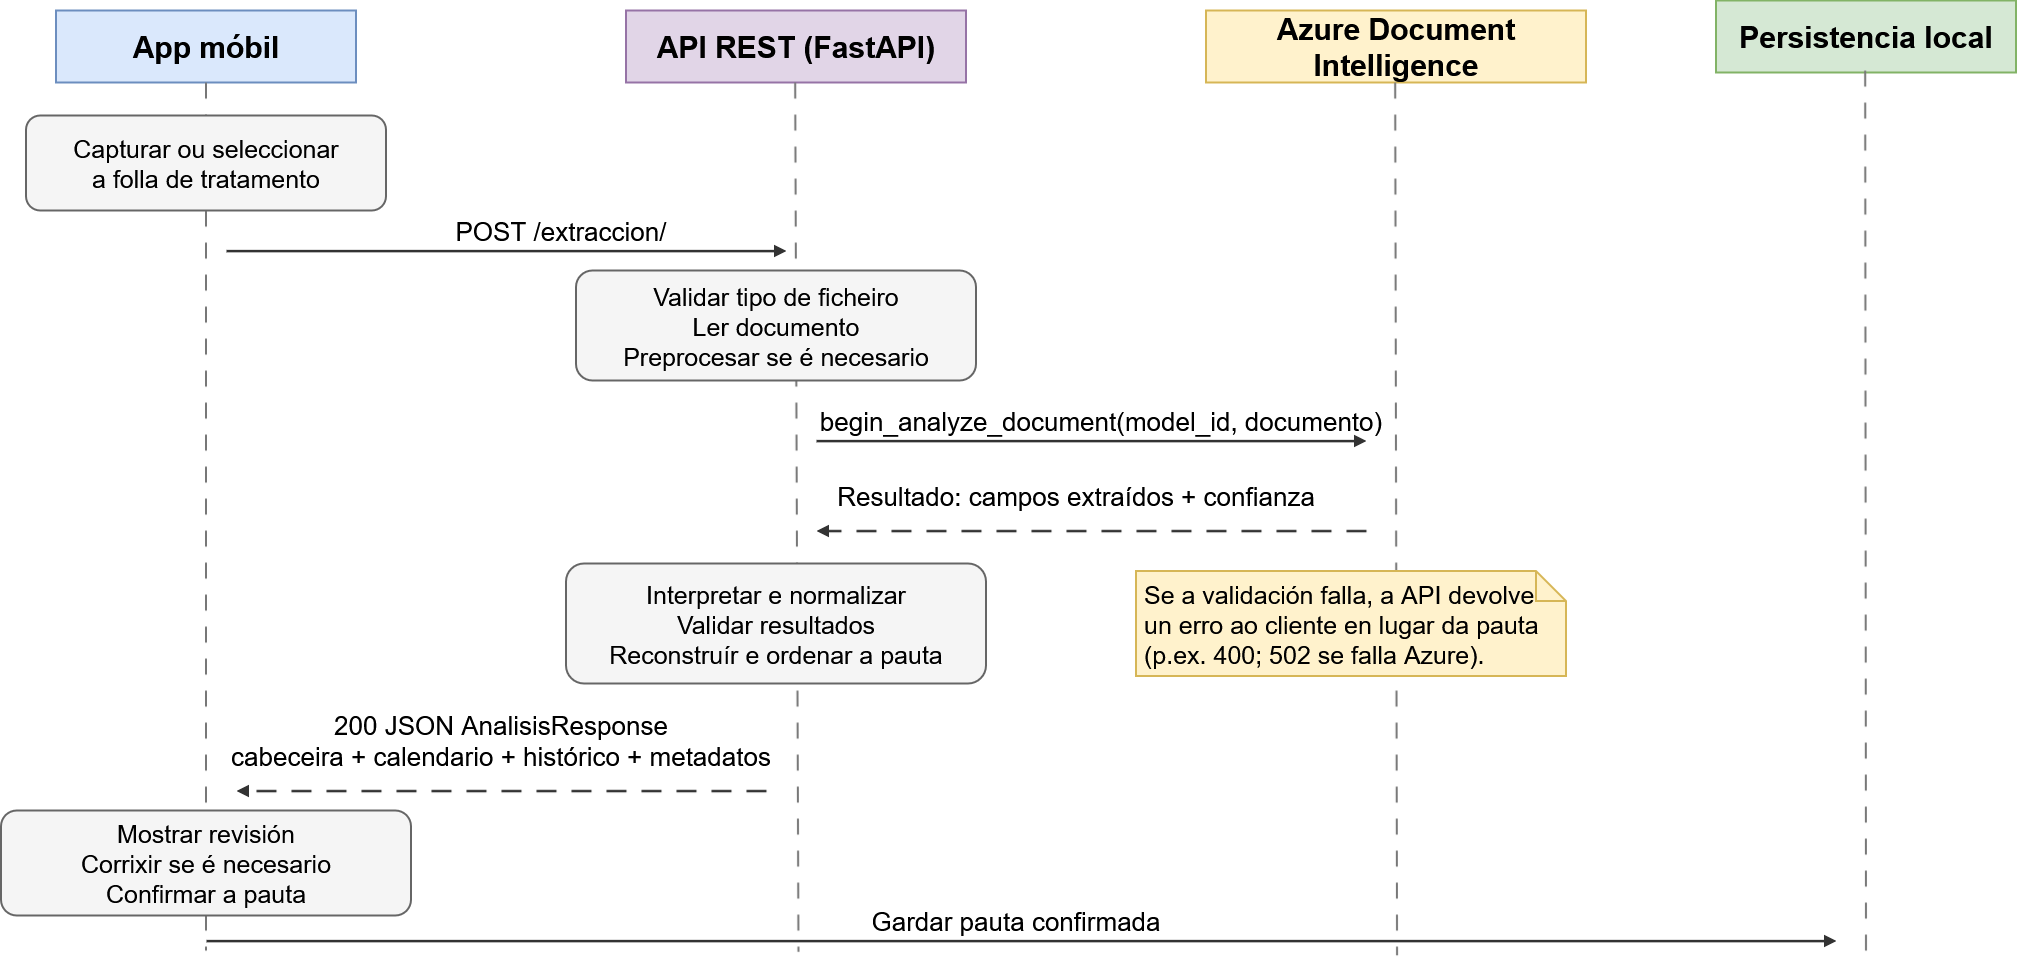
\includegraphics[width=0.9\textwidth]{imaxes/07-Deseño/secuencia_procesamento_UML.drawio.png}
    \caption{Fluxo de procesamento dunha folla de tratamento.}
    \label{fig:fluxo-procesamento}
\end{figure}

\subsection{Sincronización entre dispositivos}

Cando se produce un cambio que debe compartirse, como a confirmación dunha toma ou a incorporación dunha nova folla, o dispositivo de orixe prepara a información e cífraa empregando a clave acordada durante a vinculación. A mensaxe cifrada envíase á \gls{api}, que actúa como intermediaria e a reenvía mediante o servizo de mensaxería.

O dispositivo de destino autentica e descifra a mensaxe antes de actualizar a súa información local. Deste xeito, a \gls{api} participa no transporte sen necesitar interpretar nin almacenar o contido clínico intercambiado.

\begin{figure}[htbp]
    \centering
    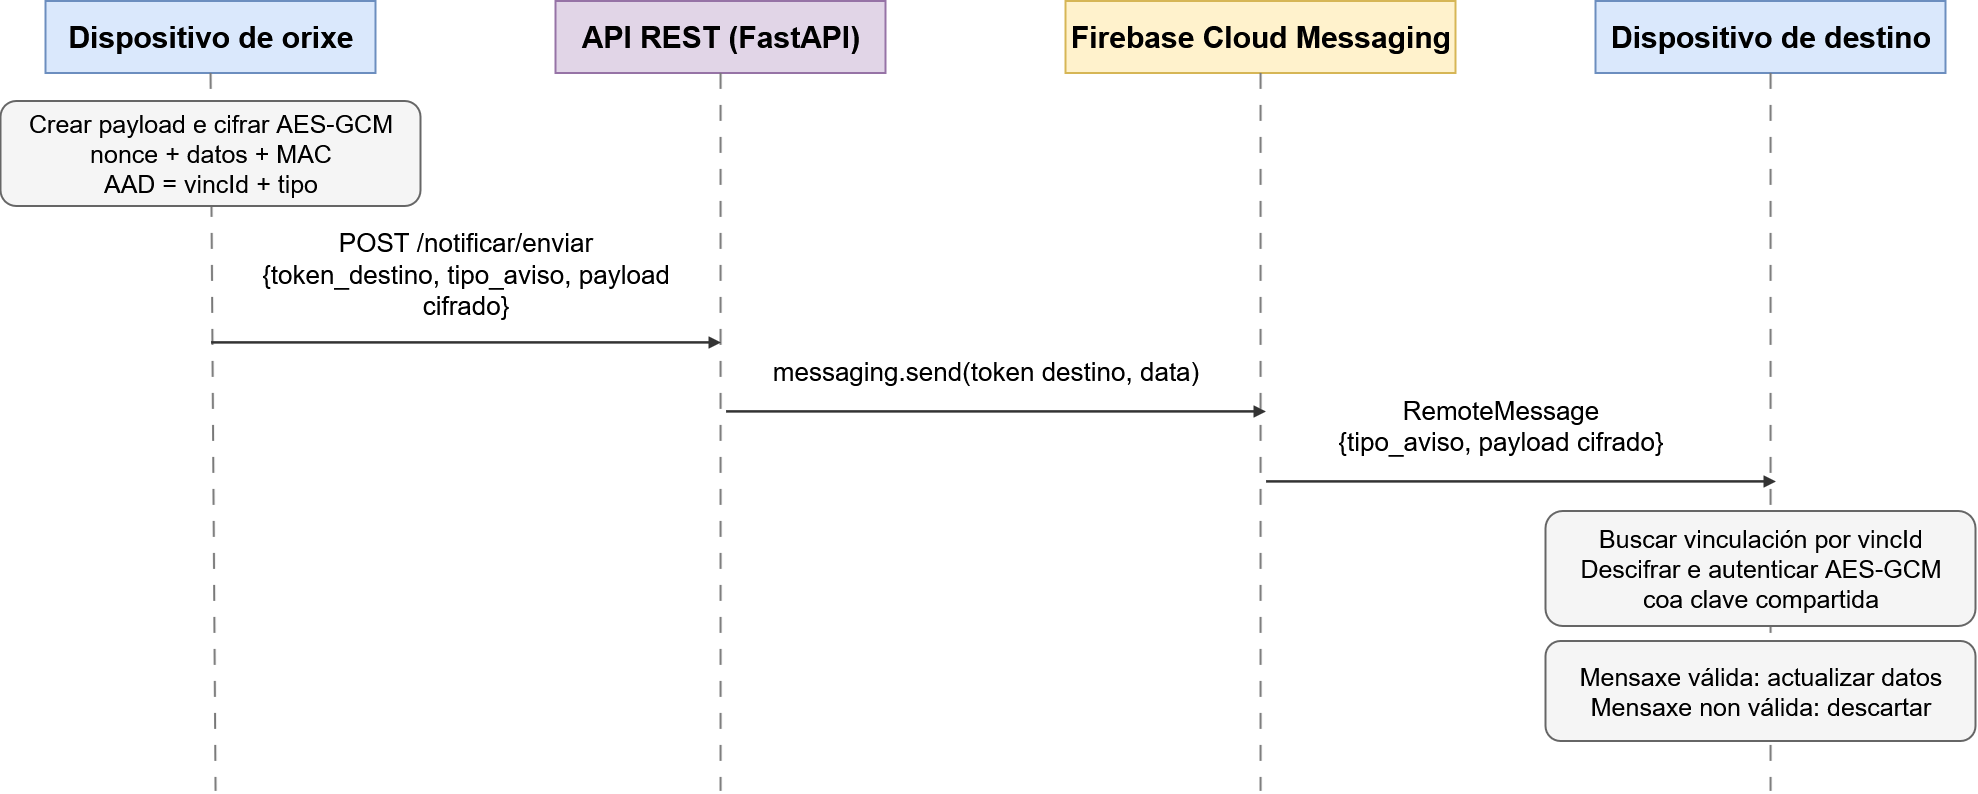
\includegraphics[width=0.9\textwidth]{imaxes/07-Deseño/secuencia_sincronizacion_UML.drawio.png}
    \caption{Fluxo de sincronización entre dispositivos vinculados.}
    \label{fig:fluxo-sincronizacion}
\end{figure}

\section{Deseño da navegación e da interface}

\subsection{Fluxo de navegación}

O primeiro acceso comeza coa selección do rol, decisión que determina as funcionalidades e o percorrido posterior. No caso do \textbf{paciente}, o fluxo inclúe a xeración do código \gls{qr}, a configuración dos permisos de dixitalización e a introdución de datos como o nome e a hora habitual da toma. A pantalla principal permite acceder á pauta, ao calendario, ao progreso, á incorporación dunha nova folla e aos axustes.

No caso da \textbf{persoa supervisora}, o proceso inicial emprega a cámara para escanear o código xerado polo paciente. Tras completar a vinculación, a pantalla principal mostra as persoas supervisadas. Ao seleccionar unha delas accédese ao seu tratamento, ao estado das tomas e ás operacións dispoñibles para a súa supervisión.

A separación por roles evita mostrar opcións que non corresponden á responsabilidade seleccionada e simplifica os percorridos máis habituais de cada tipo de persoa usuaria.

\begin{figure}[htbp]
    \centering
    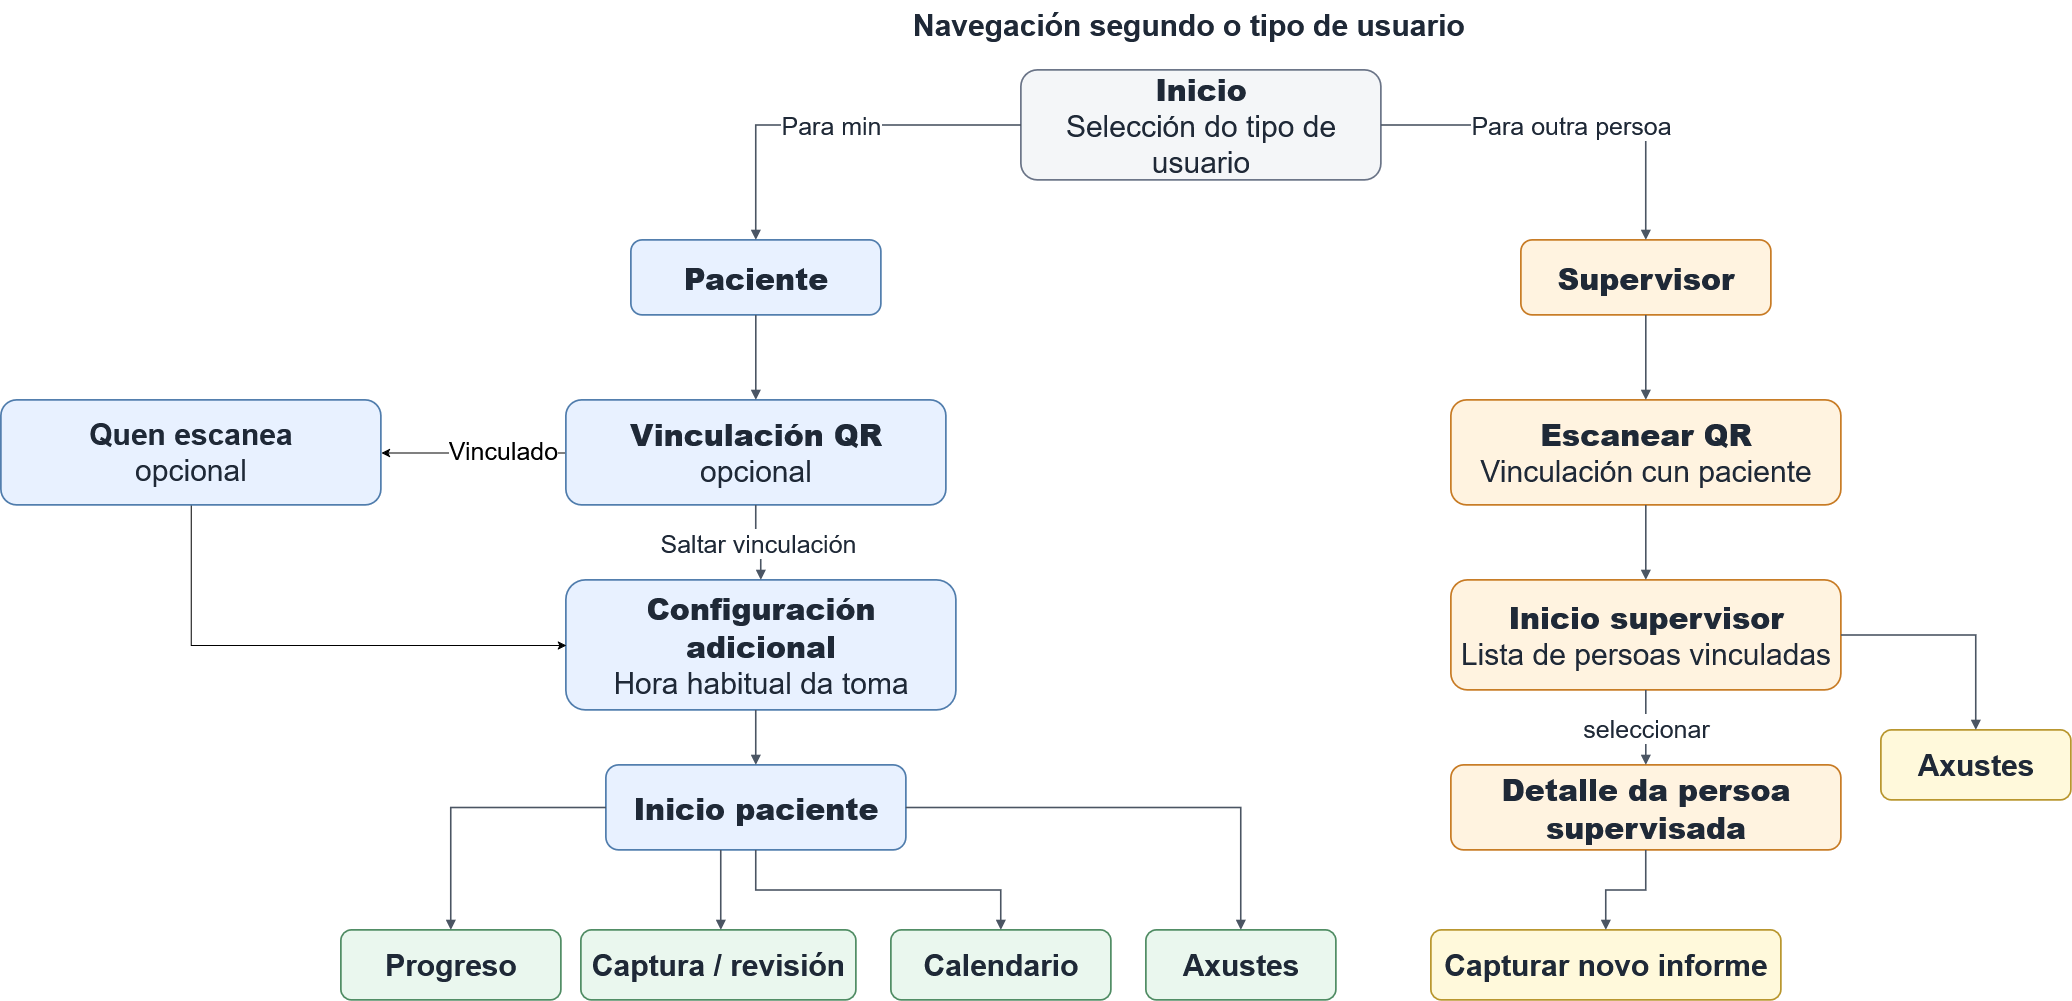
\includegraphics[width=\textwidth]{imaxes/07-Deseño/diagrama fluxo.drawio.png}
    \caption{Fluxo de navegación das pantallas segundo o tipo de usuario.}
    \label{fig:navegacion-pantallas}
\end{figure}

\subsection{Wireframes da interface}

Antes da implementación elaboráronse en Figma distintos wireframes para definir a distribución da información e comprobar os principais percorridos. Estes deseños serviron como referencia inicial, aínda que algúns elementos se adaptaron durante o desenvolvemento ao comprobar o seu funcionamento en dispositivos reais.

Na Figura~\ref{fig:wireframes-principais} móstranse os wireframes máis representativos: selección do rol, pantalla principal do paciente, incorporación dunha folla e pantalla principal da persoa supervisora. O conxunto completo, incluíndo as pantallas de vinculación, revisión, calendario, progreso e configuración, recóllese no Apéndice~\ref{app:wireframes}.

\begin{figure}[htbp]
    \centering
    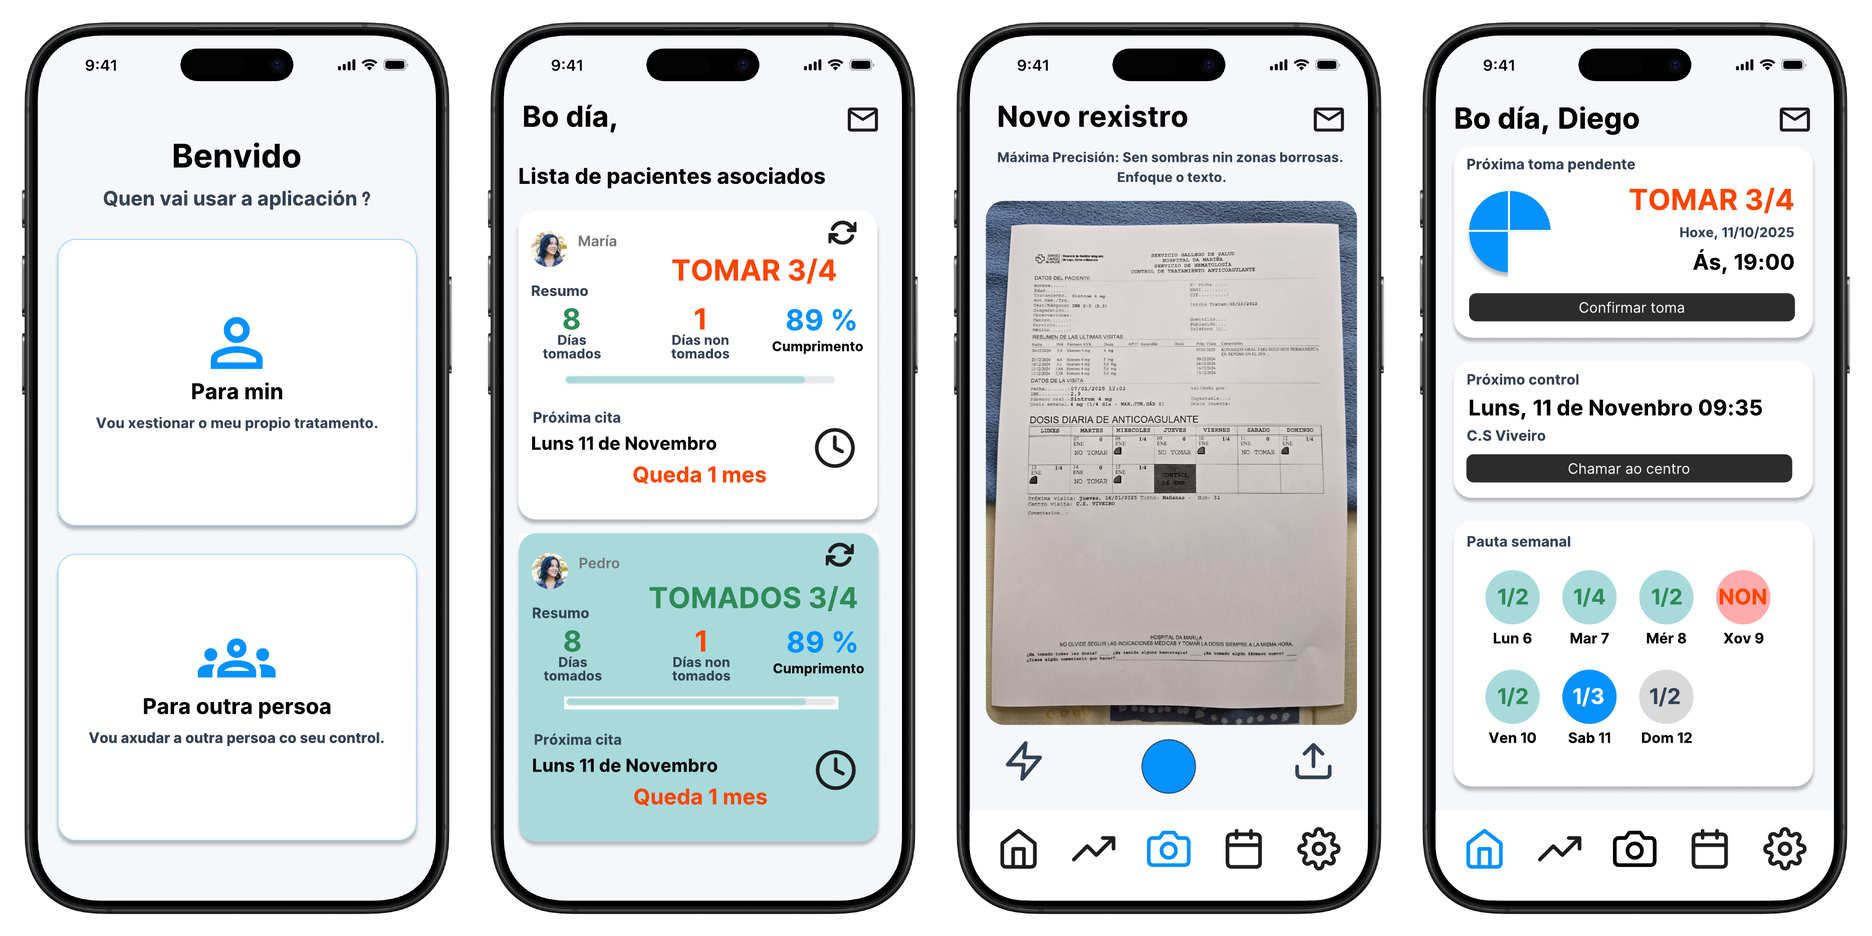
\includegraphics[width=0.90\textwidth]{imaxes/07-Deseño/wireframes_principais.png}
    \caption{Wireframes representativos da interface da aplicación.}
    \label{fig:wireframes-principais}
\end{figure}

 \chapter{Implementación}
\label{chap:implem}


\section{Implementación da API}
%meter en apéndice
% - Exemplos do JSON devolto por cada endpoint,, exemplos de código e igual unha foto do swagger e de algunha chamada.
% - Os modelos de pydantic
% - Mteer igual cousas mais concretas dos edpoint auxiliares


A \gls{api} implementouse con FastAPI e mantén separadas a configuración dos servizos externos, os puntos de entrada, os esquemas de datos e a lóxica auxiliar. 

\subsection{Inicialización e acceso aos servizos externos}

A conexión cos servizos externos realízase durante o arranque da \gls{api}, antes de que esta comece a atender peticións. Para iso emprégase o mecanismo de ciclo de vida de \textit{FastAPI}, no que se inicializan \textit{Azure Document Intelligence} e \textit{Firebase Admin} e se recuperan as credenciais necesarias para acceder a estes servizos.

A obtención das credenciais segue unha estratexia común nos dous casos. En primeiro lugar, compróbase se están dispoñibles nas variables de contorno do sistema. Este mecanismo facilita a execución da \gls{api} durante o desenvolvemento sen necesidade de acceder a servizos adicionais. Se as credenciais non están presentes, utilízase \textit{DefaultAzureCredential} para autenticarse contra \textit{Azure Key Vault} e recuperar os segredos correspondentes.

Unha vez obtida a clave de \textit{Azure Document Intelligence}, créase unha instancia de \textit{DocumentIntelligenceClient}. Esta instancia almacénase no estado da aplicación e reutilízase durante todo o seu ciclo de vida. As rutas que necesitan realizar a extracción reciben o cliente mediante o sistema de inxección de dependencias de \textit{FastAPI}, evitando así ter que crealo e configuralo para cada petición.

No caso de \textit{Firebase Admin}, as credenciais recuperadas conteñen a configuración da conta de servizo. A partir delas inicialízase o SDK de administración de Firebase. Antes de realizar esta operación compróbase se xa existe unha instancia inicializada, evitando rexistrar a aplicación máis dunha vez durante a execución. Unha vez configurado, o servizo de mensaxería de Firebase pode empregarse desde as rutas encargadas do envío de notificacións.

%Esta implementación centraliza a configuración dos servizos externos no arranque da \gls{api}, mantén a xestión das credenciais separada da lóxica das rutas e permite reutilizar os recursos xa inicializados. Ademais, a combinación de variables de contorno e \textit{Azure Key Vault} facilita o uso de configuracións diferentes segundo o contorno de execución sen incorporar credenciais directamente no código fonte.

Esta implementación centraliza a configuración dos servizos externos e mantén a xestión das credenciais separada da lóxica dos endpoints.

\subsection{Implementación do procesamento dunha folla}
A solución seleccionada no Capítulo~\ref{chap:procesamento-follas} integrouse no endpoint \textit{/extraccion/}. Ademais de  invocar ao servizo de procesamento documental, o endpoint executa as operacións necesarias para preparar e comprobar os resultados. %Meter preprocesamento

%TODO-> Meter no anexo como funciona ben o preprocesamento (Como se implementa). Revisar capitulo de procesamento 
Antes de realizar a extracción compróbase que o ficheiro se corresponda con algún dos formatos admitidos. A continuación aplícase a etapa de preprocesamento e envíase o resultado ao modelo personalizado de Azure. Se o servizo non identifica ningún documento ou a confianza global da extracción é inferior ao 60\%, a petición considérase non válida e non se constrúe a pauta.

Unha vez obtidos os campos, realízanse distintas comprobacións para evitar resultados incoherentes. A data da próxima visita compárase coa data do informe e rexéitase a extracción se é anterior. O valor do INR normalízase para admitir tanto coma como punto decimal, compróbase que poida converterse a un valor numérico, que se atope dentro dun intervalo lóxico de 0,5 a 10 e que a confianza proporcionada por Azure sexa polo menos do 80\,\%.

A táboa de doses procésase cela a cela para obter a data, a dose e a acción correspondente. Durante esta transformación compróbase que o día e o mes permitan construír unha data válida e tense en conta o cambio de ano cando a pauta pasa de decembro a xaneiro. As celas que indican \textit{NO TOMAR} convértense nunha dose cero, mentres que as identificadas como \textit{CONTROL} reciben un tratamento específico. Se non é posible recuperar correctamente a data da cela de control, emprégase a data da próxima visita. Do mesmo xeito, se a data extraída non coincide coa próxima visita, substitúese por esta para manter a coherencia entre ambos campos. Finalmente, se non se consegue recuperar ningunha entrada válida da táboa, a extracción é rexeitada.

O histórico transfórmase ao formato interno conservando unicamente as filas nas que se recuperou polo menos a data ou o INR. Unha vez procesada e validada a información, os resultados organízanse empregando os modelos de Pydantic cos que se implementou a estrutura definida no deseño. A resposta constrúese mediante \textit{AnalisisResponse}, garantindo que os datos enviados ao cliente móbil manteñan o formato establecido pola \gls{api}.

\subsection{Endpoints auxiliares}
Ademais do procesamento das follas, a \gls{api} incorpora varios endpoints auxiliares. O endpoint de centros sanitarios permite buscar os datos dun centro a partir do seu nome, empregando o catálogo almacenado na \gls{api} e admitindo pequenas variacións na denominación. O endpoint de estado permite comprobar que a \gls{api} está operativa e devolve o estado, a data e hora da consulta e a versión en execución, mentres que o de preprocesamento permite aplicar esta etapa de forma independente, sen realizar a extracción con Azure, facilitando así a comprobación do resultado xerado.

A \gls{api} tamén intervén na comunicación entre os dispositivos vinculados mediante o endpoint \textit{/notificar/enviar}. Este recibe o token do dispositivo destinatario, o tipo de aviso e un \textit{payload} que xa foi cifrado no dispositivo de orixe. A API non necesita interpretar o seu contido, senón que actúa como intermediaria e emprega Firebase Cloud Messaging para reenvialo ao destinatario. Para determinados avisos engádese unha notificación visible cun título e unha mensaxe xenéricos, mantendo a información sensible exclusivamente no \textit{payload} cifrado.

\subsection{Tratamento de erros}
Diferéncianse os erros segundo a súa orixe. Os ficheiros ou resultados que non superan as comprobacións da extracción devolven un erro 400 \textit{(Bad Request)}, mentres que os erros de validación dos parámetros de entrada son xestionados por FastAPI mediante unha resposta 422\textit{ (Unprocessable Entity)}. Os fallos de comunicación con Azure devolven un 502 \textit{(Bad Gateway)} e os erros inesperados da aplicación un 500 \textit{(Internal Server Error)}. Noutros endpoints empréganse tamén códigos específicos, como o 404\textit{ (Not Found)} cando non se localiza un centro sanitario ou o 503 \textit{(Service Unavailable)} cando non se pode acceder ao catálogo. Esta diferenciación permite que o cliente identifique mellor a causa do problema e mostre unha mensaxe adecuada á persoa usuaria.

\section{Implementación do cliente móbil}

%Revisa rintroducció
%A aplicación móbil implementouse en Flutter seguindo o patrón MVVM definido no deseño. As vistas xestionan a interacción coa persoa usuaria, os modelos de vista manteñen o estado e coordinan as operacións, e os modelos representan os datos empregados pola aplicación. Os servizos encapsulan o acceso á \gls{api}, á persistencia, ás notificacións e á sincronización.

\subsection{Inicialización da aplicación}

Antes de mostrar a interface, a aplicación inicializa os servizos necesarios para o seu funcionamento mediante a clase \textit{InicializadorAplicacion}.

Neste proceso configúrase Firebase, prepárase a recepción de mensaxes tanto en primeiro como en segundo plano e solicítanse os permisos necesarios para as notificacións. Tamén se recupera do almacenamento seguro a información da configuración previa, como o rol seleccionado e se o proceso inicial xa foi completado.

A partir destes datos determínase a pantalla que debe mostrarse ao iniciar a aplicación. Se a configuración está pendente, accédese ao fluxo inicial. Se xa foi completada, móstrase directamente a interface de paciente ou de persoa supervisora. No caso do paciente, tamén se restauran os recordatorios asociados á pauta activa.

\subsection{Incorporación e revisión dunha folla de tratamento}
A incorporación dunha folla de tratamento divídese en 3 pasos: o envñio á \gls{api}, a revisión dos resultados e a confirmación final. O ficheiro pode obterse mediante a cámara, a galería ou o selector de documentos. O modelo de vista de captura mantén o estado do proceso e xestiona os posibles erros.

O envío realízase mediante \textit{ApiService}, empregando unha petición \gls{http} de tipo \textit{multipart}. Se a extracción é correcta, o \gls{json} devolto transfórmase nun \textit{AnaliseModel}. Se se produce un erro, a mensaxe recibida trasládase á interface para informar á persoa usuaria.

Antes de gardar a pauta, os datos pasan por unha fase de revisión xestionada por \textit{RevisionPauta}. Esta permite modificar, engadir ou eliminar días, cambiar doses e marcar días de control. Tamén comproba que a pauta non estea baleira, que as datas sexan válidas e non estean duplicadas, e que as doses teñan un formato admitido.

Tras a confirmación, o comportamento depende do dispositivo. Se a folla foi incorporada polo paciente, gárdase como pauta activa, reprograman os recordatorios e notifícase o cambio ás persoas supervisoras vinculadas. Se foi incorporada desde o dispositivo supervisor, a pauta revisada envíase ao paciente para que sexa almacenada como tratamento activo.






 \include{contido/demo}
%\include{contido/...}
 \chapter{Conclusións}
\label{chap:conclusions}

\lettrine{O} obxectivo principal deste traballo foi desenvolver unha solución móbil que facilitase o seguimento diario do tratamento anticoagulante con Sintrom, reducindo a dependencia da folla física e simplificando tanto a interpretación da pauta como o control das tomas. Para alcanzar este obxectivo desenvolveuse SintromApp, formada por un cliente móbil implementado con Flutter e unha \gls{api} desenvolvida con FastAPI, complementados con diferentes servizos para o procesamento documental, as notificacións e a comunicación entre dispositivos.

Unha das partes máis relevantes do traballo foi o estudo das alternativas para automatizar a lectura das follas de tratamento. Ao longo do proxecto avaliáronse diferentes técnicas de recoñecemento óptico de caracteres, visión artificial e procesamento documental. As probas realizadas mostraron que non era suficiente con recuperar correctamente o texto presente no documento, xa que resultaba imprescindible conservar tamén a relación entre cada data e a súa dose para poder reconstruír a pauta de forma fiable. Finalmente, a comparación realizada permitiu seleccionar o modelo \textit{Template} de Azure AI Document Intelligence, que mostrou un comportamento máis estable na extracción da estrutura das follas e, especialmente, da táboa de doses.

A partir desta extracción implementouse o procesamento necesario para transformar a información obtida nunha pauta estruturada que puidese ser empregada directamente pola aplicación. Para iso foi necesario interpretar datas e doses, identificar os días de control, resolver cambios de ano, comprobar determinados valores e ordenar cronoloxicamente o calendario. Este proceso permitiu pasar dunha folla pensada para a súa consulta visual a unha representación dixital apta para o seguimento diario do tratamento.

En relación cos obxectivos formulados ao inicio do proxecto, considérase que estes se cumpriron de maneira satisfactoria. A aplicación permite incorporar unha folla mediante unha fotografía, unha imaxe almacenada no dispositivo ou un documento \gls{pdf}, reducindo a necesidade de introducir manualmente a información. Os datos extraídos poden revisarse e corrixirse antes de seren incorporados como pauta activa, o que resulta especialmente importante ao tratarse de información relacionada coa medicación. Unha vez gardada, a persoa usuaria pode consultar a dose correspondente a cada día, acceder ao calendario e ao histórico e visualizar a evolución do tratamento.

Tamén se incorporaron mecanismos destinados a facilitar o cumprimento da pauta. A aplicación permite configurar unha hora habitual para a toma e programa recordatorios para as doses pendentes. A persoa usuaria pode confirmar cada toma e o sistema conserva o seu estado, distinguindo entre tomas realizadas, realizadas fóra da hora prevista, pendentes ou non realizadas. Ademais, incorporouse un modo sinxelo co obxectivo de reducir a complexidade da interface nos casos nos que se precise unha interacción máis directa coa aplicación.

Outro dos obxectivos consistía en facilitar a supervisión do tratamento. Para iso desenvolveuse un sistema de vinculación entre pacientes e persoas supervisoras mediante códigos \gls{qr}. Esta relación permite compartir cambios relevantes da pauta e do estado das tomas entre dispositivos e posibilita tamén que unha persoa supervisora incorpore unha nova folla en nome dun paciente vinculado. Deste xeito, o seguimento non queda limitado ao propio dispositivo do paciente e pode realizarse tamén de forma remota.

A privacidade da información foi outro dos aspectos considerados durante o deseño e a implementación. Os datos do tratamento almacénanse principalmente de forma local e a \gls{api} non mantén unha base de datos central coa información clínica das persoas usuarias. A configuración sensible e as claves asociadas ás vinculacións almacénanse mediante mecanismos de almacenamento seguro, mentres que a información intercambiada entre dispositivos se cifra antes do seu envío. Desta forma, os servizos empregados para transportar as mensaxes non necesitan interpretar o contido clínico transmitido.

A solución desenvolvida foi comprobada mediante probas unitarias, de integración e de interface, complementadas con probas manuais en dispositivos Android. A \gls{api} alcanzou unha cobertura global do 96,1\,\%, mentres que o cliente móbil obtivo un 72,8\,\%. A diferenza entre ambos valores débese principalmente ás funcionalidades do cliente que dependen directamente do dispositivo, como a cámara, as notificacións locais ou determinadas operacións de sincronización, que foron verificadas tamén mediante probas manuais. Estas comprobacións permitiron validar os principais fluxos da aplicación, incluíndo a incorporación e revisión dunha folla, a persistencia da pauta, a confirmación das tomas, a vinculación entre dispositivos e a recepción das notificacións.

Durante o desenvolvemento foi necesario afrontar diferentes dificultades técnicas. A principal estivo relacionada coa variabilidade das condicións nas que pode capturarse unha folla e coa necesidade de reconstruír correctamente a información dunha táboa a partir dos datos extraídos automaticamente. A avaliación das distintas alternativas mostrou que unha boa taxa de recoñecemento de caracteres non implica necesariamente que unha ferramenta sexa adecuada para este problema, xa que a conservación da estrutura do documento resulta fundamental. Outro reto importante foi coordinar a persistencia local, os recordatorios e a sincronización entre dispositivos sen depender dun servidor central que almacenase a información do tratamento.

A solución presenta tamén limitacións que deben terse en conta. O sistema de extracción foi deseñado e probado sobre o formato das follas de tratamento empregadas polo SERGAS, polo que non pode asumirse o mesmo comportamento con documentos doutros organismos ou cunha estrutura diferente. A calidade da captura pode afectar igualmente ao resultado da extracción e, por este motivo, a aplicación incorpora unha etapa de revisión antes de gardar a información. Ademais, aínda que se realizaron probas funcionais e comprobacións de interface, non se levou a cabo un estudo formal de usabilidade con participantes externos nin unha validación clínica por parte de profesionais sanitarios. Estas comprobacións serían necesarias antes de considerar a utilización da aplicación nun contexto real.

Como posibles liñas de traballo futuro, poderíase ampliar a extracción para admitir outros formatos de follas de tratamento, incrementar a robustez ante documentos capturados en condicións desfavorables e continuar mellorando os mecanismos de sincronización entre dispositivos. Tamén resultaría de interese realizar estudos de usabilidade con pacientes e persoas supervisoras, especialmente con persoas de idade avanzada, co obxectivo de avaliar o modo sinxelo e detectar posibles barreiras de interacción. Finalmente, unha evolución máis ambiciosa da solución podería estudar a integración cos sistemas oficiais de saúde.

En conxunto, o proxecto permitiu desenvolver unha solución funcional que integra desenvolvemento móbil, deseño e implementación de \glspl{api}, procesamento documental, persistencia local, cifrado, mensaxería e probas. Máis alá do resultado técnico, o traballo permitiu comprobar a importancia de avaliar experimentalmente as tecnoloxías antes de incorporalas á solución definitiva e de adaptar as decisións de deseño ás características concretas do problema. SintromApp constitúe así unha base funcional sobre a que se podería continuar traballando para avanzar cara a unha ferramenta máis completa de apoio ao seguimento do tratamento anticoagulante.

 %%%%%%%%%%%%%%%%%%%%%%%%%%%%%%%%%%%%%%%%
 % Apéndices, glosarios e bibliografía  %
 %%%%%%%%%%%%%%%%%%%%%%%%%%%%%%%%%%%%%%%%

 \appendix
 \appendixpage
% \chapter{Material adicional}
\label{chap:adicional}

\lettrine{E}{xemplo} de capítulo con formato de apéndice, onde se pode
incluír material adicional que non teña cabida no corpo principal do
documento, suxeito á limitación de 80 páxinas establecida no
regulamento de TFGs.

\Blindtext


\chapter{Descrición dos casos de uso principais}
\label{chapapd:descricion-casos-principais}

Nesta sección descríbense con maior detalle os casos de uso máis representativos do funcionamento do sistema. Seleccionáronse aqueles que recollen os principais fluxos da aplicación e as interaccións máis relevantes entre o paciente, o supervisor, a API e os servizos externos.

\subsubsection{CU-02: Vincular paciente e supervisor}

\begin{description}
    \item[Actores:] Paciente e supervisor.

    \item[Precondicións:] Ambos os dispositivos teñen a aplicación iniciada, dispoñen de conexión á rede e completaron a selección do seu rol. O supervisor dispón de permisos para utilizar a cámara.

    \item[Disparador:] O paciente selecciona a opción de xerar un código QR para vincular un supervisor.

    \item[Fluxo principal:] \hfill
    \begin{enumerate}
        \item A aplicación informa de que a persoa vinculada poderá consultar a información compartida, recibir avisos e dixitalizar novas follas no nome do paciente.
        \item O paciente solicita a xeración do código QR, aceptando os permisos asociados á vinculación.
        \item A aplicación do paciente xera un código QR cos identificadores e os datos de seguridade necesarios.
        \item O supervisor abre a opción de lectura, escanea o código e o sistema comproba a súa validez.
        \item Os dispositivos intercambian as credenciais necesarias para establecer unha canle de comunicación segura.
        \item O paciente pasa a figurar como vinculado no dispositivo do supervisor.
        \item A vinculación actívase e os dispositivos poden intercambiar o estado do tratamento de forma protexida.
        \item O supervisor pode consultar os datos sincronizados e dixitalizar novas follas no nome do paciente.
    \end{enumerate}

    \item[Fluxos alternativos:] Se o código QR ten un formato incorrecto ou xa foi empregado, a aplicación rexeita a vinculación e solicita xerar outro código. En caso de fallo de conexión ou se as credenciais de seguridade non se poden verificar, a operación cancélase indicando o motivo. O paciente pode omitir este proceso e empregar a aplicación de maneira autónoma.

    \item[Postcondicións:] Establécese unha relación de confianza entre os dispositivos. A vinculación permite ao supervisor consultar a información compartida, recibir avisos e dixitalizar novas follas no nome do paciente. Estes permisos poden retirarse mediante a revogación da vinculación desde os axustes da aplicación.
\end{description}

O intercambio de información necesario para establecer a vinculación entre os dous dispositivos represéntase no diagrama de secuencia da Figura~\ref{fig:cu02-vinculacion}.

\begin{figure}
    \centering
    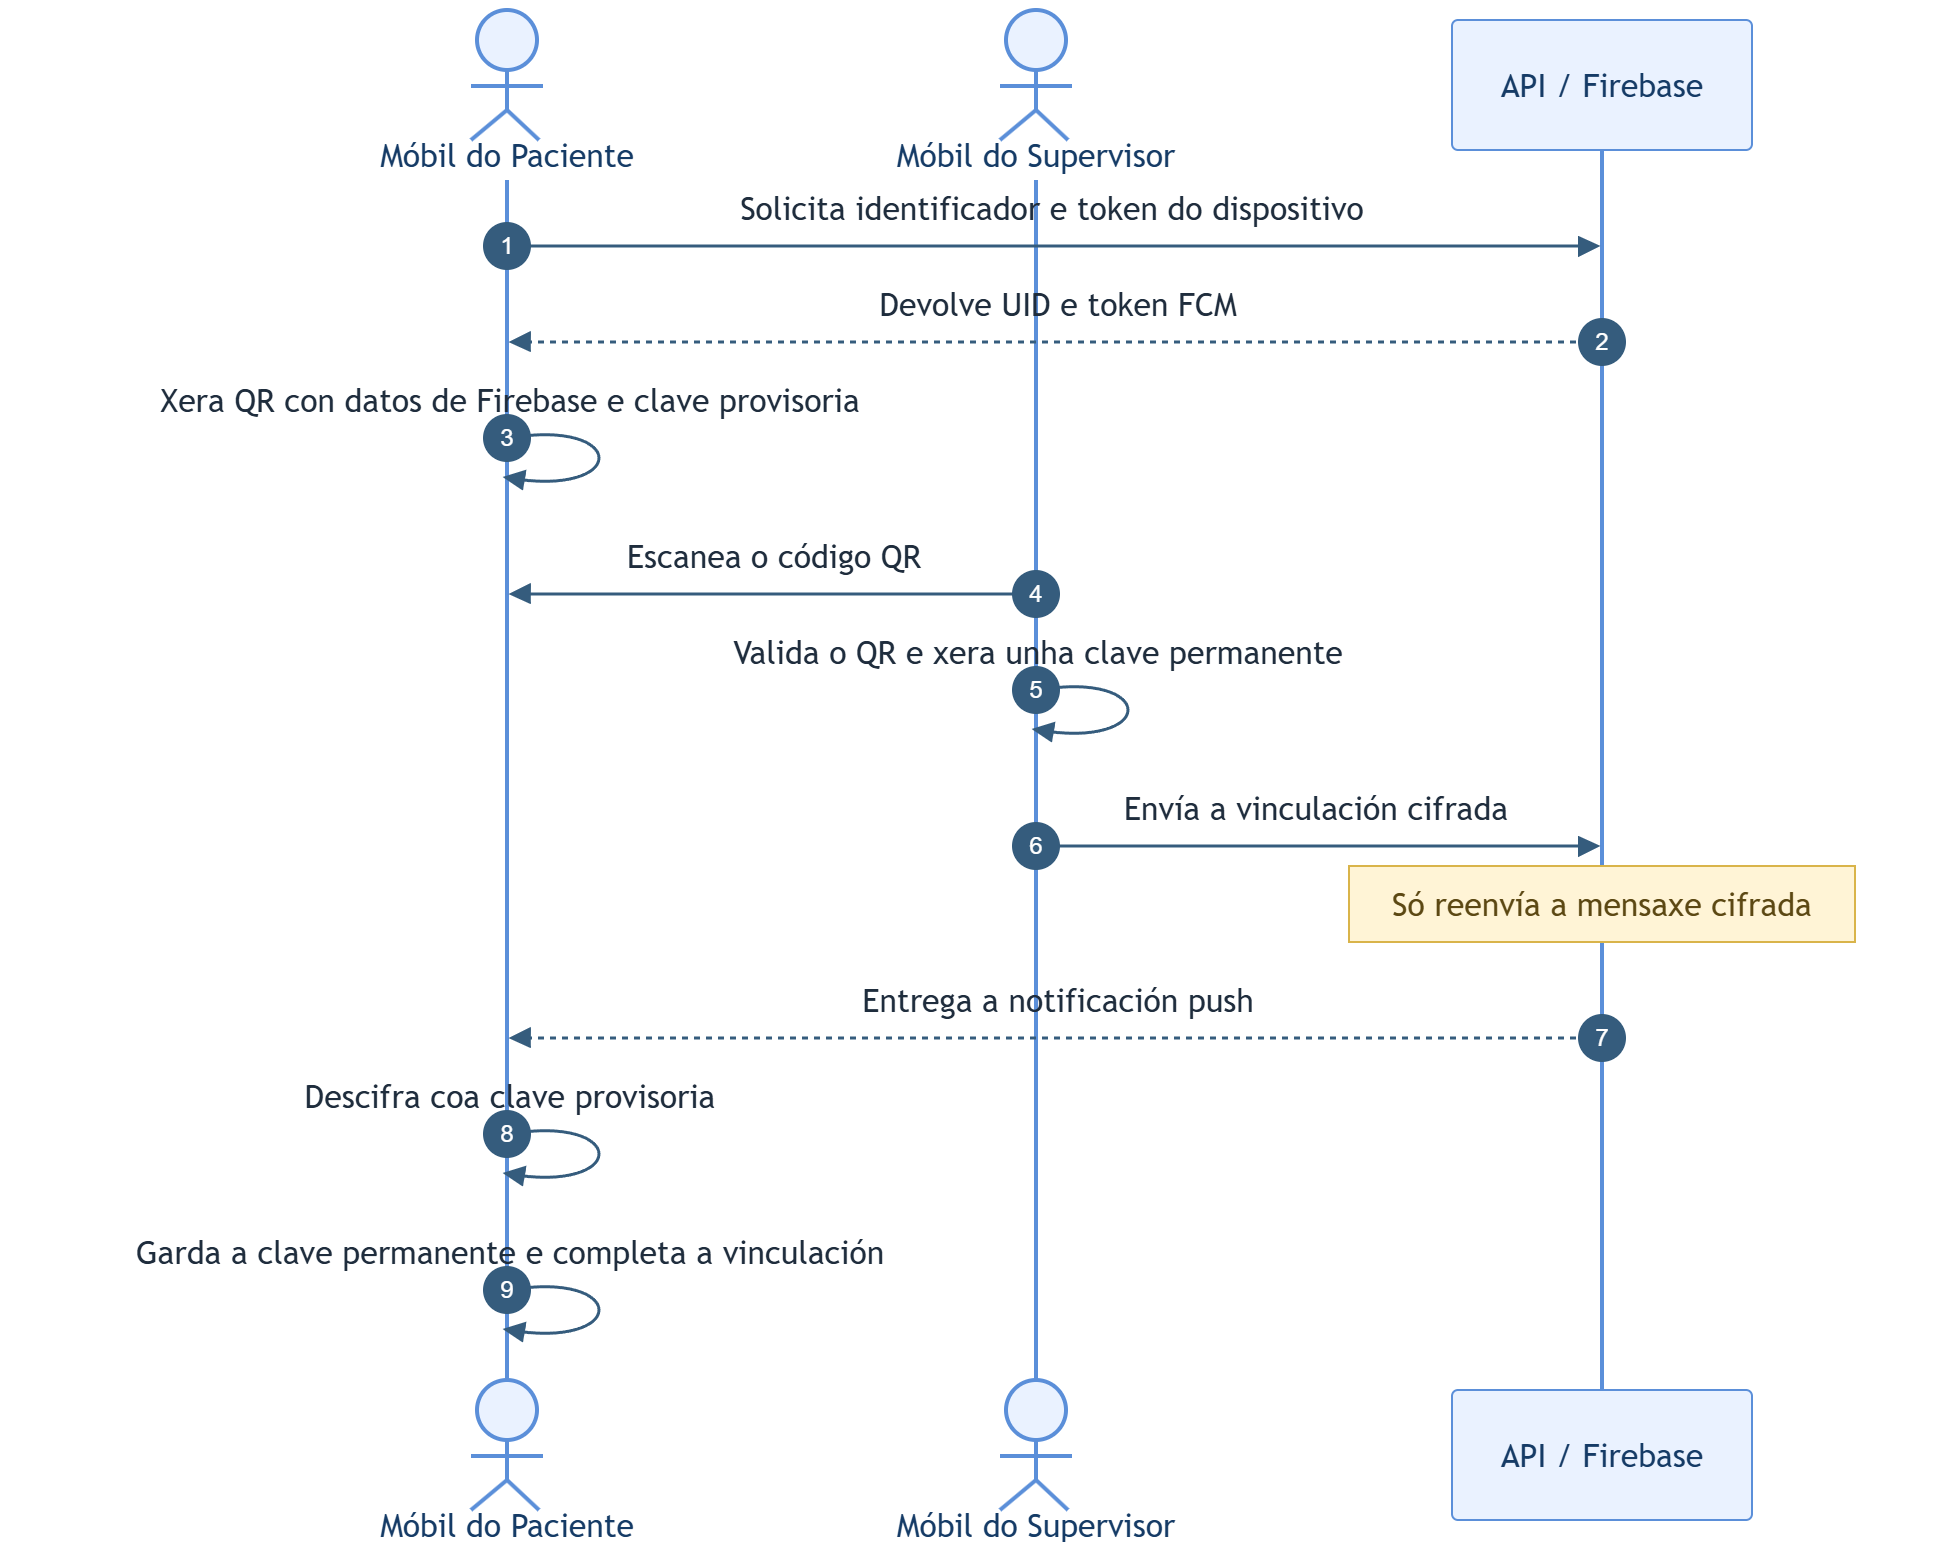
\includegraphics[width=1\linewidth]{imaxes/04-Analise/CU02-Vinculacion.png}
    \caption{Diagrama de secuencia do proceso de vinculación entre o paciente e o supervisor (CU-02).}
    \label{fig:cu02-vinculacion}
\end{figure}
\FloatBarrier

\subsubsection{CU-04: Procesar unha folla de tratamento}

\begin{description}
    \item[Actor principal:] Paciente ou supervisor vinculado.

    \item[Precondicións:] A aplicación está iniciada, existe conexión á rede e o actor dispón dunha folla de tratamento lexible. Se a acción a realiza un supervisor, este debe manter unha vinculación activa co paciente e telo seleccionado previamente.

    \item[Disparador:] O usuario preme a opción de engadir ou actualizar unha folla de tratamento.

    \item[Fluxo principal:] \hfill
    \begin{enumerate}
        \item O usuario selecciona a orixe do documento: cámara, galería ou ficheiro PDF.
        \item A aplicación comproba que o formato e o tamaño sexan compatibles.
        \item O ficheiro envíase á API mediante unha petición HTTPS.
        \item A API preprocesa a imaxe, extrae os datos estruturados e aplica as regras de validación.
        \item Se a API procesa correctamente o documento, a aplicación recibe os datos extraídos e gárdaos localmente.
        \item A nova pauta móstrase na interface principal.
        \item Se existen outros dispositivos vinculados, a actualización empaquétase de forma segura e sincronízase automaticamente con eles.
    \end{enumerate}

    \item[Fluxos alternativos:] Se o documento non é lexible, a API rexeita o formato ou faltan datos obrigatorios, o proceso interrómpese. A aplicación mantén intacta a pauta anterior, mostra unha mensaxe de erro descritiva e solicita repetir a captura. Se a extracción se completa pero falla a sincronización, a pauta permanece gardada no dispositivo local e infórmase do erro de rede.

    \item[Postcondicións:] A nova pauta consolídase no dispositivo que realizou a operación e sincronízase de forma segura cos dispositivos vinculados. O documento orixinal descártase tras a súa análise e non se almacena de forma persistente no servidor.
\end{description}

As diferentes etapas do procesamento e o comportamento do sistema ante un resultado correcto ou un erro represéntanse no diagrama de actividade da Figura~\ref{fig:cu04-procesar-folla}.

\begin{figure}[H]
    \centering
    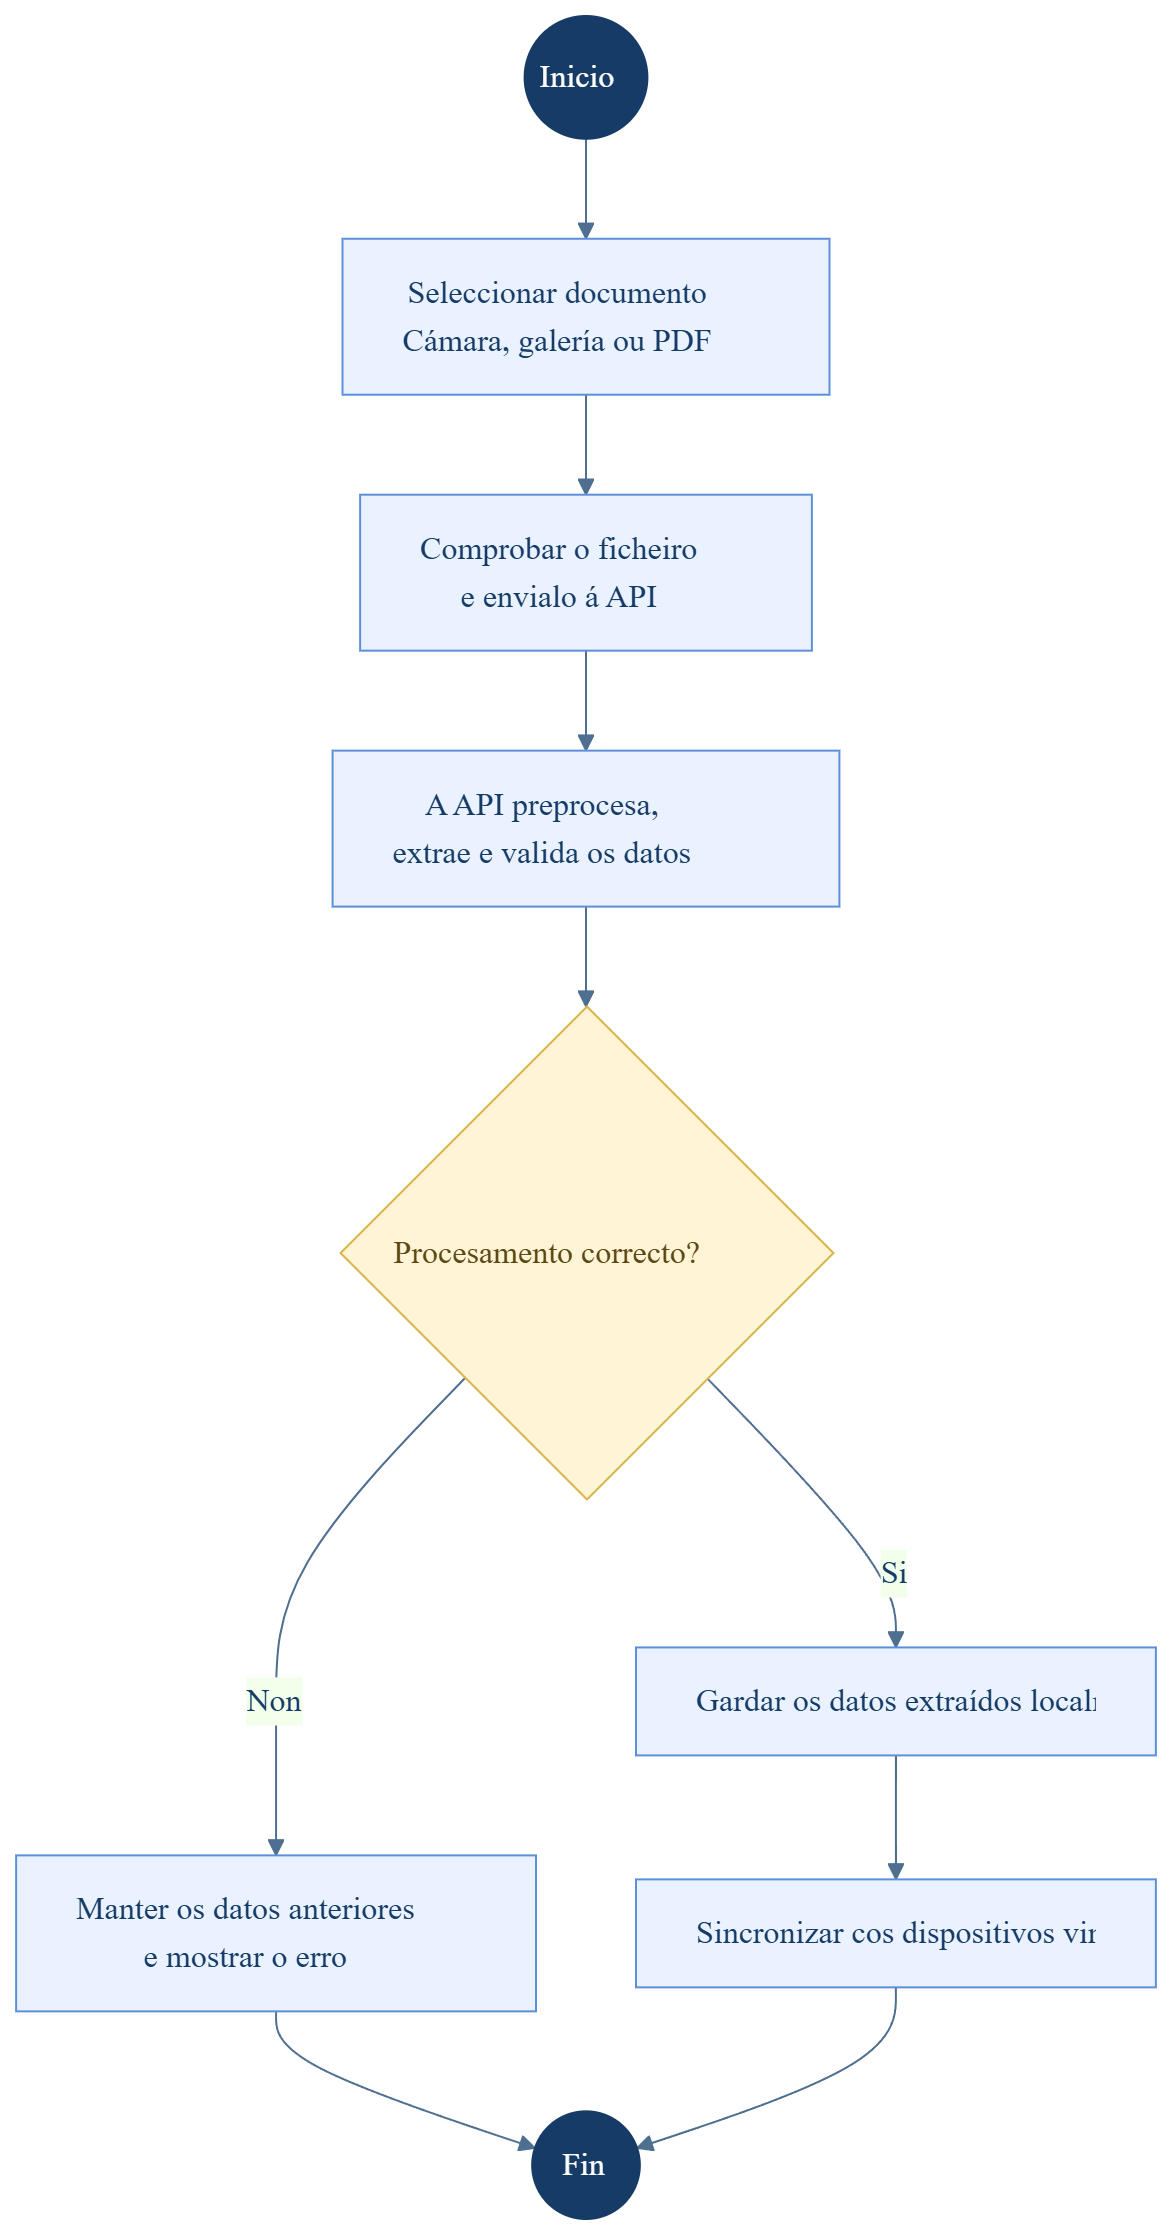
\includegraphics[width=0.6\linewidth]{imaxes/04-Analise/CU04-Procesar-Folla.png}
    \caption{Diagrama de actividade do procesamento dunha folla de tratamento (CU-04).}
    \label{fig:cu04-procesar-folla}
\end{figure}
\FloatBarrier

\subsubsection{CU-06: Confirmar unha toma}

\begin{description}
    \item[Actor principal:] Paciente.

    \item[Precondicións:] O sistema conta cunha pauta activa que inclúe unha dose prescrita para o día en curso.

    \item[Disparador:] O paciente activa o control de confirmación da toma diaria na interface.

    \item[Fluxo principal:] \hfill
    \begin{enumerate}
        \item A aplicación identifica a dose asignada para a xornada actual.
        \item Rexistra a confirmación xunto coa data e a hora exactas na base de datos local.
        \item Avalía a puntualidade da toma en comparación coa hora habitual configurada nas preferencias.
        \item Actualiza a pantalla de inicio, o calendario e as métricas de adherencia.
        \item Se existen supervisores vinculados, notifícase o evento aos seus dispositivos de forma segura.
    \end{enumerate}

    \item[Fluxos alternativos:] A interface non permite confirmar unha toma cando a pauta indica que ese día non debe tomarse medicación ou corresponde unicamente a un control médico. En ausencia de conexión, a confirmación permanece rexistrada localmente, pero a comunicación cos supervisores non pode completarse ata recuperar a conectividade.

    \item[Postcondicións:] A toma pasa ao estado de confirmada e incorpórase ao historial local de tomas. Os supervisores que reciban correctamente a actualización poden consultar o novo estado.
\end{description}

Os posibles estados asociados á toma diaria e as transicións producidas pola confirmación represéntanse na Figura~\ref{fig:cu06-confirmar-toma}.

\begin{figure}[H]
    \centering
    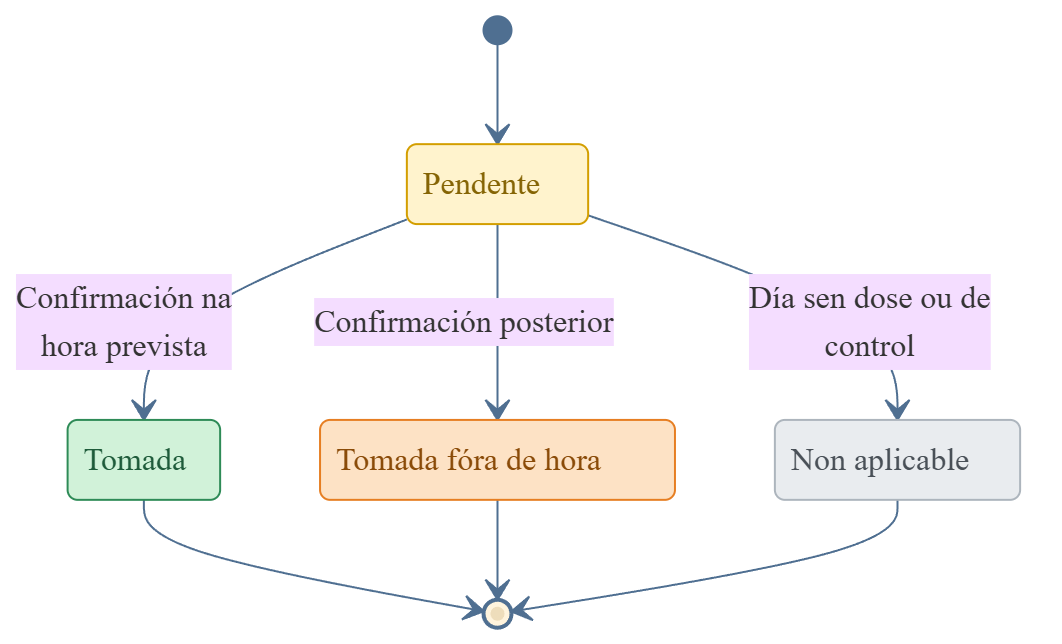
\includegraphics[width=0.6\linewidth]{imaxes/04-Analise/CU06-Confirmar-Toma.png}
    \caption{Diagrama de estados asociado á confirmación dunha toma diaria (CU-06).}
    \label{fig:cu06-confirmar-toma}
\end{figure}
\FloatBarrier

\subsubsection{CU-10: Supervisar un paciente}

\begin{description}
    \item[Actor principal:] Supervisor.

    \item[Precondicións:] O supervisor mantén unha vinculación activa con polo menos un paciente que xa compartiu información do seu tratamento.

    \item[Disparador:] O supervisor selecciona un perfil de paciente na pantalla principal.

    \item[Fluxo principal:] \hfill
    \begin{enumerate}
        \item A aplicación carga o panel de estado do paciente seleccionado.
        \item O supervisor visualiza a dose do día, o estado da toma e a data da seguinte visita médica.
        \item O supervisor pode consultar o calendario e as gráficas de evolución dispoñibles.
        \item O supervisor pode iniciar a captura dunha nova folla para actualizar a pauta do paciente seleccionado.
        \item Se o documento se procesa correctamente, a nova pauta envíase de forma segura ao dispositivo do paciente.
    \end{enumerate}

    \item[Fluxos alternativos:] Se o paciente aínda non dixitalizou ningunha folla, móstrase unha mensaxe indicando que non hai información dispoñible. Se a vinculación foi revogada, o sistema bloquea o acceso ao perfil, impide dixitalizar novas follas no seu nome e deixa de aceptar actualizacións asociadas á relación eliminada.

    \item[Postcondicións:] A consulta non modifica o estado do tratamento. Se o supervisor procesa unha nova folla, a pauta actualízase e sincronízase co paciente vinculado.
\end{description}

\subsubsection{CU-11: Sincronizar cambios e recibir avisos}

\begin{description}
    \item[Actor principal:] Paciente ou supervisor.

    \item[Precondicións:] Existe unha vinculación activa e comprobada entre os dispositivos.

    \item[Disparador:] Prodúcese un cambio que debe ser comunicado, como a confirmación dunha toma, a actualización dunha pauta, unha modificación da configuración ou a revogación dunha vinculación.

    \item[Fluxo principal:] \hfill
    \begin{enumerate}
        \item O dispositivo de orixe empaqueta a actualización e cífraa, garantindo a súa privacidade.
        \item A API recibe a petición de envío e encamíñaa ao destinatario correspondente sen acceder ao contido da mensaxe.
        \item O dispositivo destinatario recibe a notificación e verifica a autenticidade e a integridade da mensaxe.
        \item Se a comprobación é correcta, descifra a información, aplícaa e actualiza a interface.
    \end{enumerate}

    \item[Fluxos alternativos:] Se a orixe é descoñecida, a mensaxe foi alterada durante o tránsito ou non cumpre os controis de seguridade, o dispositivo descártaa sen modificar os datos locais. Se non hai conexión á rede, o envío non pode completarse, pero consérvanse os datos gardados no dispositivo de orixe para permitir unha sincronización posterior.

    \item[Postcondicións:] O dispositivo destinatario incorpora unha actualización procedente dunha vinculación válida. A API e o servizo de mensaxería interveñen unicamente como intermediarios e non acceden á información clínica en claro.
\end{description}

O proceso de envío dunha actualización cifrada e o papel da API e de Firebase como intermediarios represéntanse no diagrama de secuencia da Figura~\ref{fig:cu11-sincronizacion-avisos}.

\begin{figure}
    \centering
    \includegraphics[width=1\linewidth]{imaxes/04-Analise/cu11-sincronizacion-avisos.png}
    \caption{Diagrama de secuencia da sincronización segura de cambios e avisos entre dispositivos (CU-11).}
    \label{fig:cu11-sincronizacion-avisos}
\end{figure}
\FloatBarrier

 \chapter{Deseño}
\label{app:deseno-detallado}

\section{Wireframes}
\label{app:wireframes}

Nesta sección recóllense os wireframes elaborados durante a fase de deseño, organizados segundo os principais fluxos de interacción da aplicación. A Figura~\ref{fig:wireframes-configuracion} mostra as pantallas asociadas á configuración inicial e á vinculación entre dispositivos; a Figura~\ref{fig:wireframes-paciente} recolle o fluxo de incorporación dunha folla e o acceso á pauta por parte do paciente; a Figura~\ref{fig:wireframes-seguimento} presenta as principais pantallas empregadas para o seguimento do tratamento; e a Figura~\ref{fig:wireframes-supervisor} agrupa as interfaces relacionadas co perfil supervisor e os axustes da aplicación. Finalmente, a Figura~\ref{fig:wireframes-modo-sinxelo-anexo} recolle os wireframes correspondentes ao modo sinxelo.

% ============================================================
% CONFIGURACIÓN INICIAL
% ============================================================

\begin{figure}[h]
    \centering

    \begin{subfigure}[t]{0.23\textwidth}
        \centering
        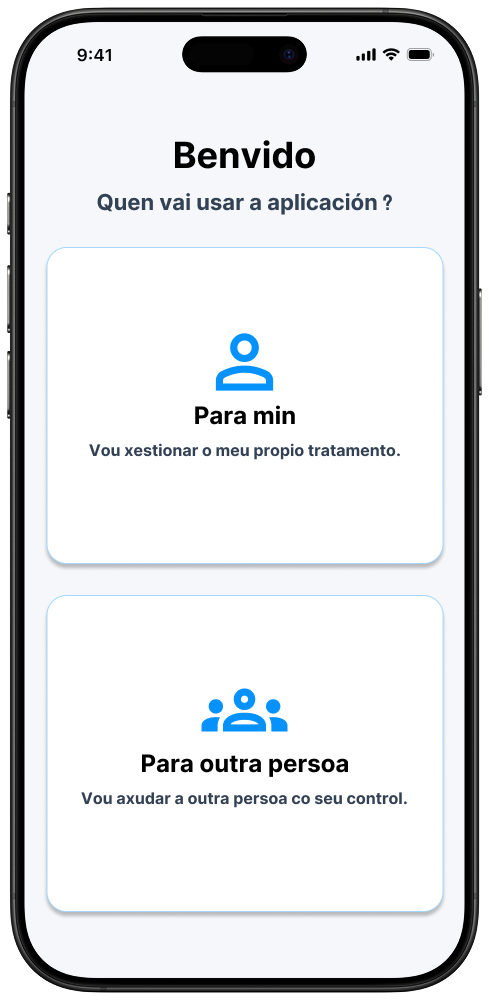
\includegraphics[width=\linewidth]
        {imaxes/07-Deseño/anexo/wireframes/Pantalla setup.png}
        \caption{Selección do rol.}
        \label{fig:wireframe-seleccion-rol}
    \end{subfigure}
    \hfill
    \begin{subfigure}[t]{0.23\textwidth}
        \centering
        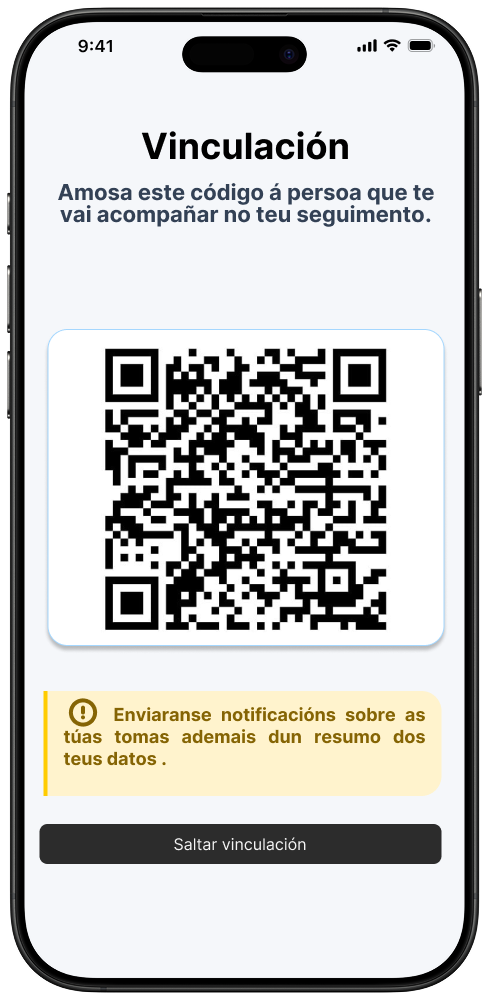
\includegraphics[width=\linewidth]
        {imaxes/07-Deseño/anexo/wireframes/Pantalla setup 2.png}
        \caption{Vinculación do paciente.}
        \label{fig:wireframe-vinculacion-paciente}
    \end{subfigure}
    \hfill
    \begin{subfigure}[t]{0.23\textwidth}
        \centering
        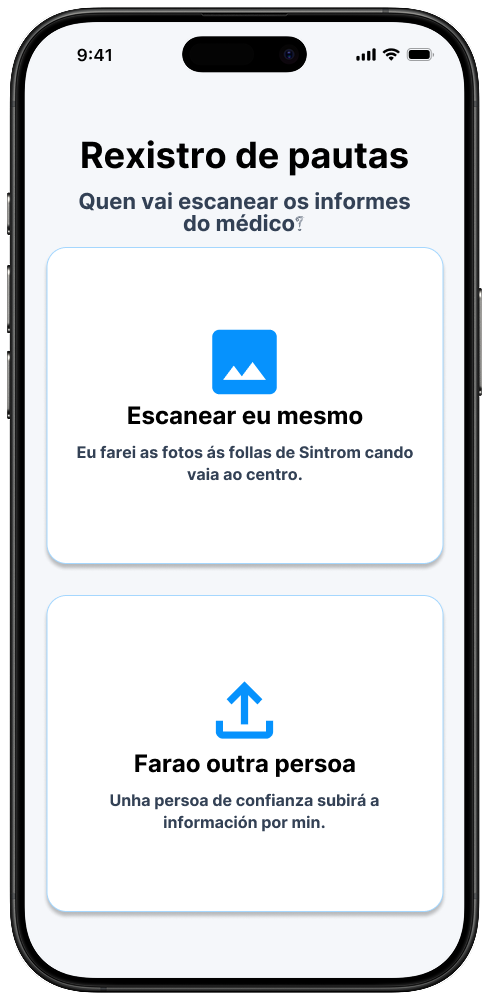
\includegraphics[width=\linewidth]
        {imaxes/07-Deseño/anexo/wireframes/Pantalla setup 3.png}
        \caption{Selección do rexistro das pautas.}
        \label{fig:wireframe-seleccion-rexistro-pautas}
    \end{subfigure}
    \hfill
    \begin{subfigure}[t]{0.23\textwidth}
        \centering
        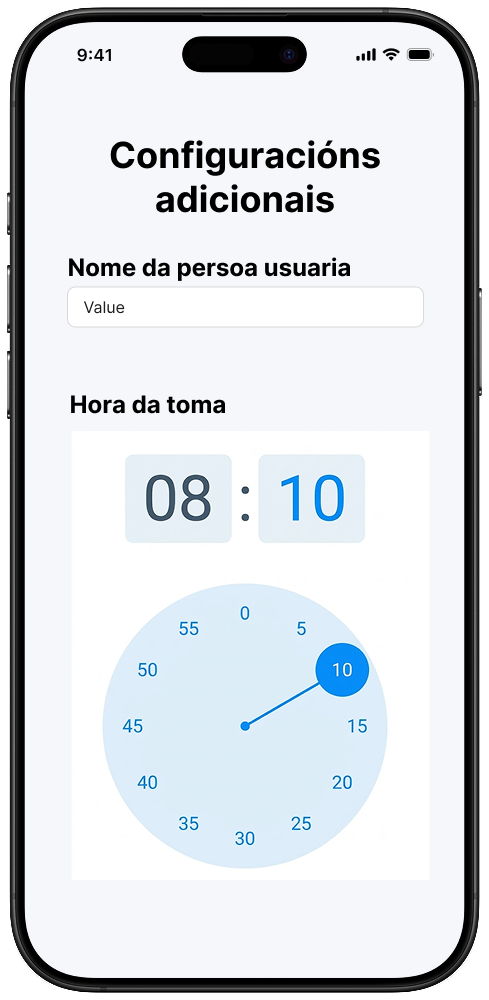
\includegraphics[width=\linewidth]
        {imaxes/07-Deseño/anexo/wireframes/Config adicionais.png}
        \caption{Configuración adicional.}
        \label{fig:wireframe-configuracion-adicional}
    \end{subfigure}

    \caption{Wireframes correspondentes á configuración inicial do paciente.}
    \label{fig:wireframes-configuracion}
\end{figure}


% ============================================================
% INCORPORACIÓN DA FOLLA E PAUTA DO PACIENTE
% ============================================================

\begin{figure}[h]
    \centering

    \begin{subfigure}[t]{0.23\textwidth}
        \centering
        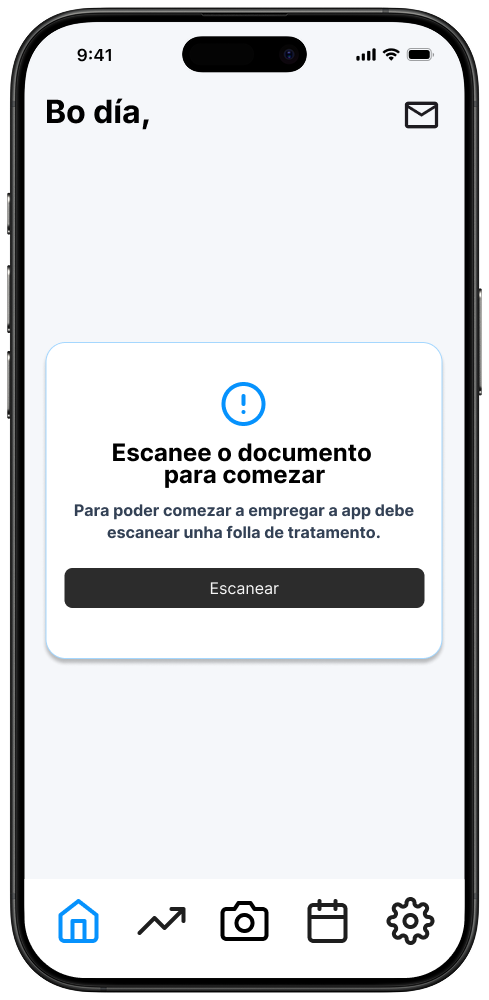
\includegraphics[width=\linewidth]
        {imaxes/07-Deseño/anexo/wireframes/Pantalla inicio vacía.png}
        \caption{Inicio sen pauta.}
        \label{fig:wireframe-inicio-sen-pauta}
    \end{subfigure}
    \hfill
    \begin{subfigure}[t]{0.23\textwidth}
        \centering
        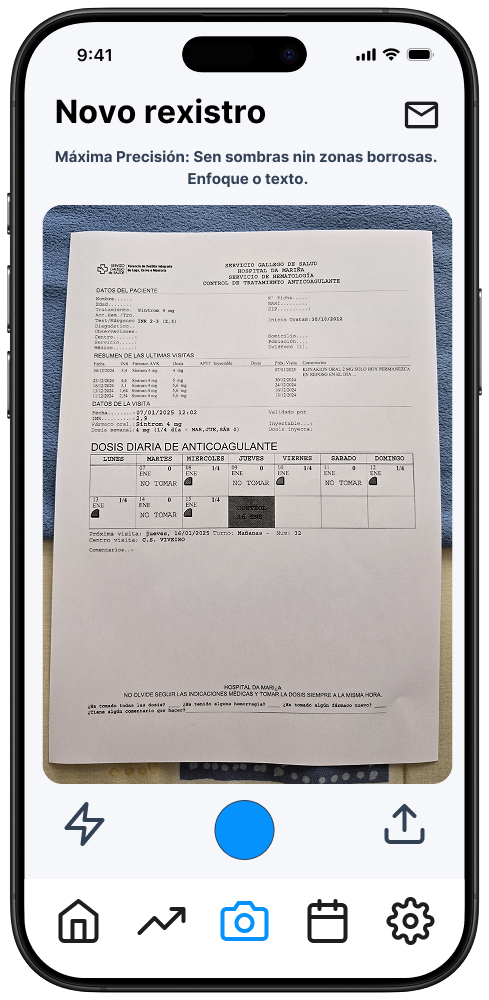
\includegraphics[width=\linewidth]
        {imaxes/07-Deseño/anexo/wireframes/Saca foto.png}
        \caption{Captura da folla.}
        \label{fig:wireframe-captura-folla}
    \end{subfigure}
    \hfill
    \begin{subfigure}[t]{0.23\textwidth}
        \centering
        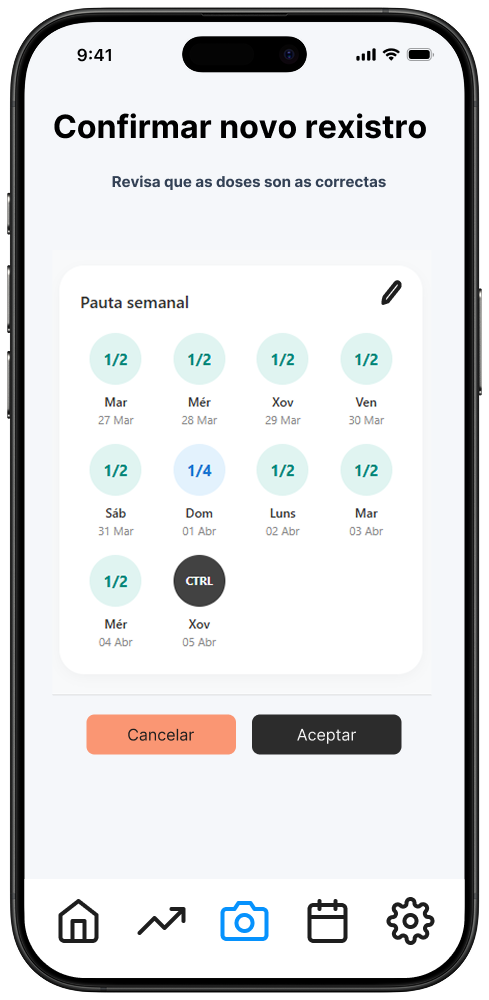
\includegraphics[width=\linewidth]
        {imaxes/07-Deseño/anexo/wireframes/Revisar toma.png}
        \caption{Revisión da pauta.}
        \label{fig:wireframe-revision-pauta}
    \end{subfigure}
    \hfill
    \begin{subfigure}[t]{0.23\textwidth}
        \centering
        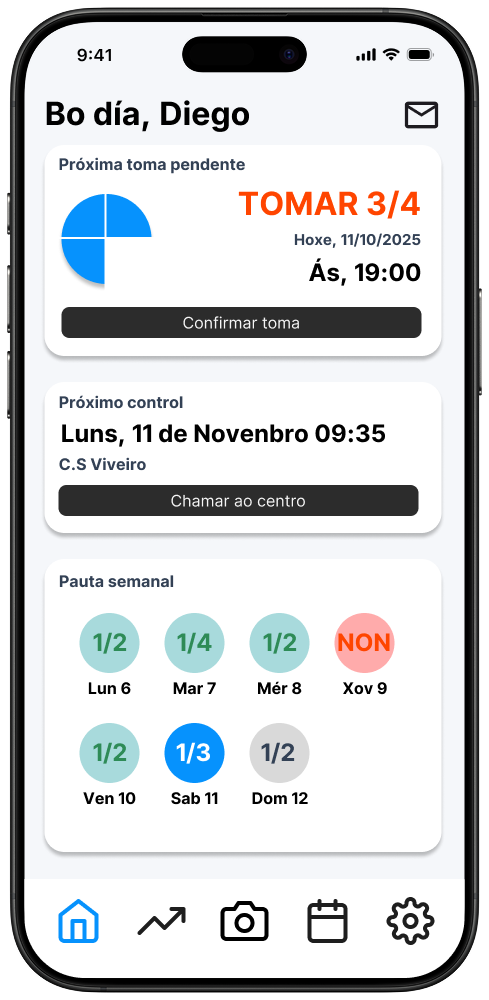
\includegraphics[width=\linewidth]
        {imaxes/07-Deseño/anexo/wireframes/Pantalla inicio.png}
        \caption{Inicio cunha toma pendente.}
        \label{fig:wireframe-inicio-paciente}
    \end{subfigure}

    \caption{Wireframes do fluxo de incorporación dunha folla e presentación da pauta ao paciente.}
    \label{fig:wireframes-paciente}
\end{figure}


% ============================================================
% SEGUIMENTO DO TRATAMENTO
% ============================================================

\begin{figure}[h]
    \centering

    \begin{subfigure}[t]{0.23\textwidth}
        \centering
        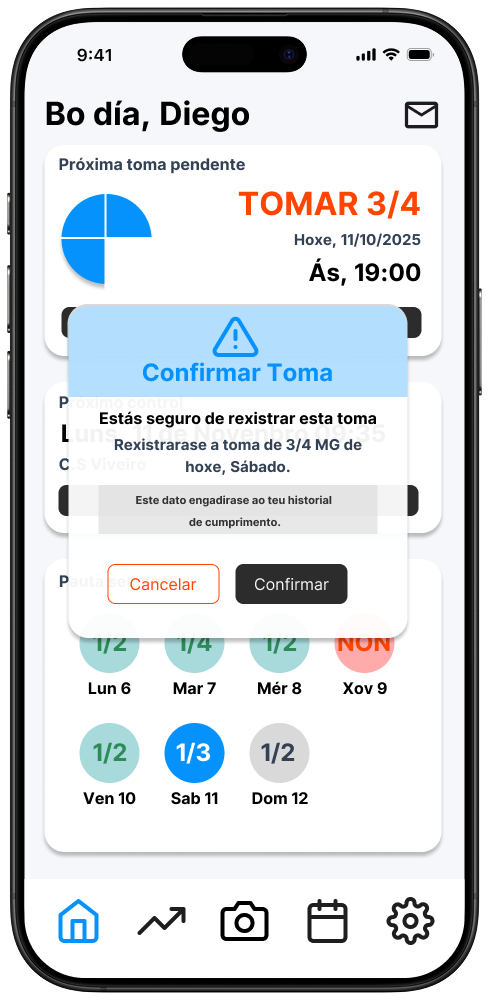
\includegraphics[width=\linewidth]
        {imaxes/07-Deseño/anexo/wireframes/Pantalla inicio Aviso.png}
        \caption{Confirmación dunha toma.}
        \label{fig:wireframe-confirmacion-toma}
    \end{subfigure}
    \hfill
    \begin{subfigure}[t]{0.23\textwidth}
        \centering
        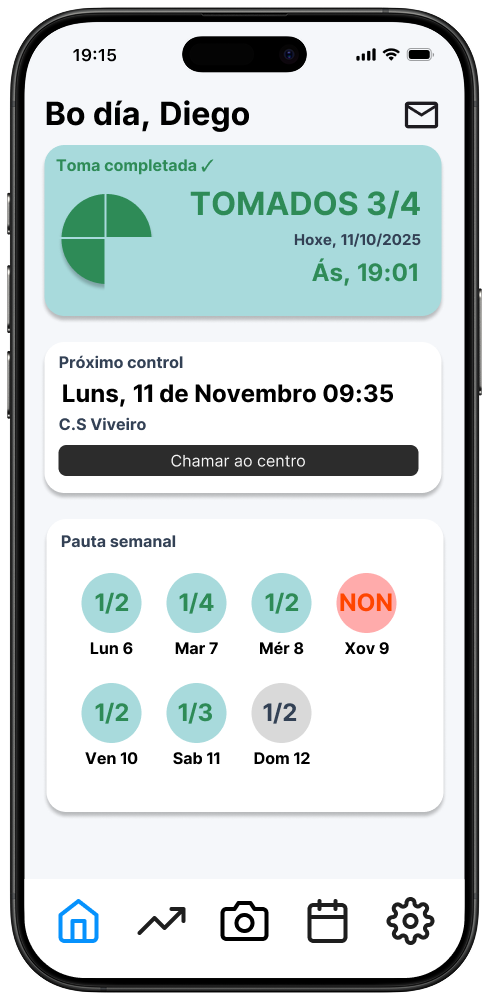
\includegraphics[width=\linewidth]
        {imaxes/07-Deseño/anexo/wireframes/Pantalla inicio 2.png}
        \caption{Toma confirmada.}
        \label{fig:wireframe-inicio-toma-confirmada}
    \end{subfigure}
    \hfill
    \begin{subfigure}[t]{0.23\textwidth}
        \centering
        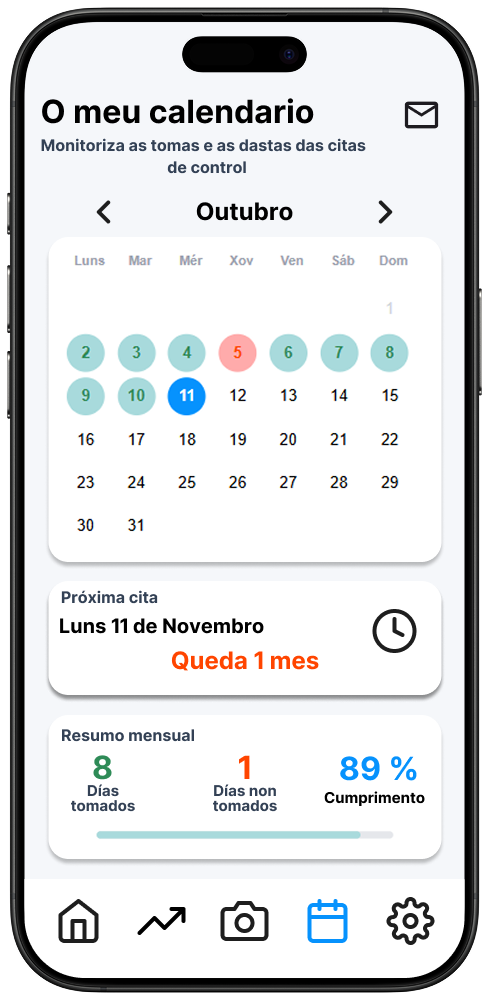
\includegraphics[width=\linewidth]
        {imaxes/07-Deseño/anexo/wireframes/Calendario.png}
        \caption{Calendario.}
        \label{fig:wireframe-calendario}
    \end{subfigure}
    \hfill
    \begin{subfigure}[t]{0.28\textwidth}
        \centering
        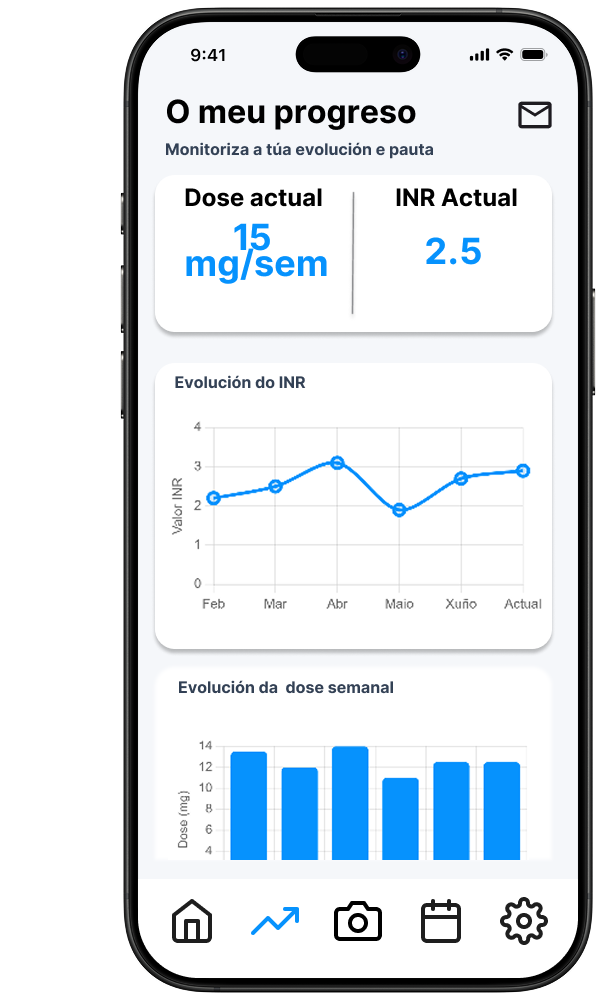
\includegraphics[width=\linewidth]
        {imaxes/07-Deseño/anexo/wireframes/O meu progreso.png}
        \caption{Progreso do tratamento.}
        \label{fig:wireframe-progreso}
    \end{subfigure}

    \caption{Wireframes das principais interfaces de seguimento do tratamento.}
    \label{fig:wireframes-seguimento}
\end{figure}


% ============================================================
% SUPERVISOR E AXUSTES
% ============================================================

\begin{figure}[h]
    \centering

    \begin{subfigure}[t]{0.23\textwidth}
        \centering
        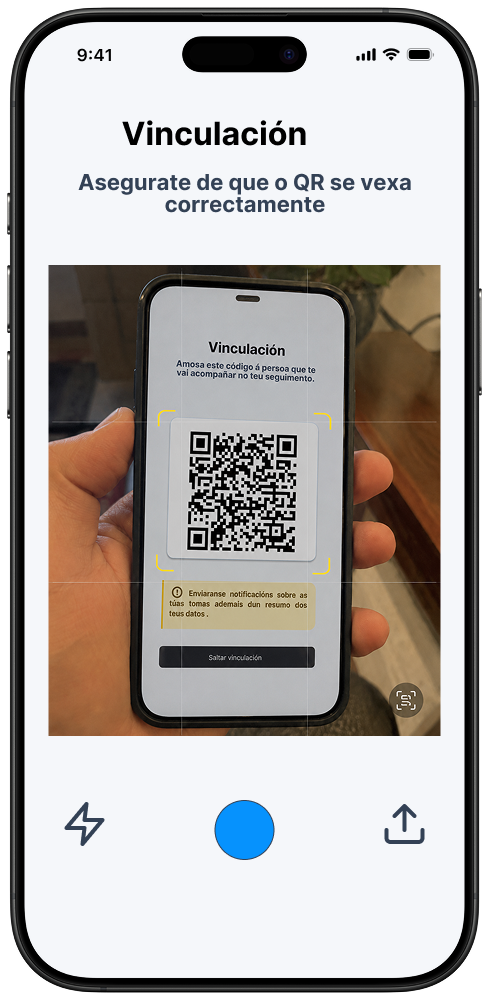
\includegraphics[width=\linewidth]
        {imaxes/07-Deseño/anexo/wireframes/Escaneo QR.png}
        \caption{Escaneo do código QR.}
        \label{fig:wireframe-escaneo-qr}
    \end{subfigure}
    \hfill
    \begin{subfigure}[t]{0.23\textwidth}
        \centering
        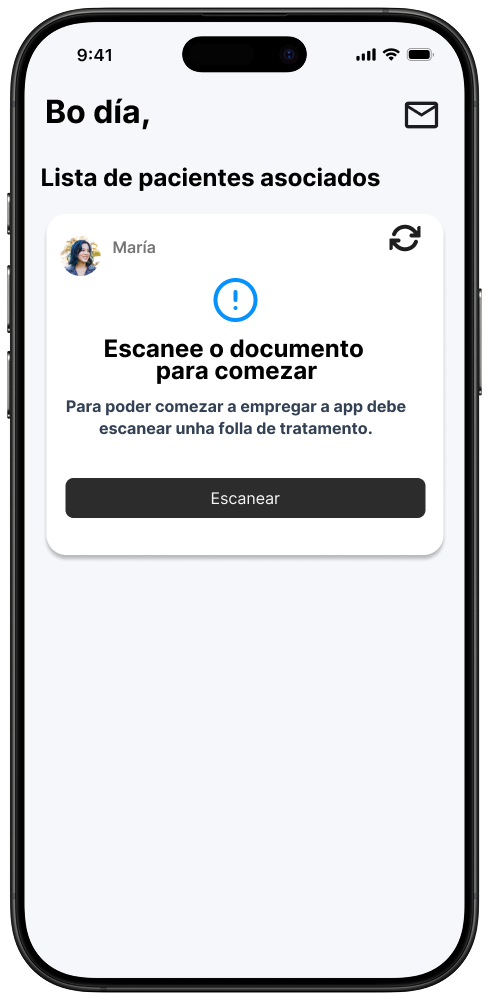
\includegraphics[width=\linewidth]
        {imaxes/07-Deseño/anexo/wireframes/Inicio supervisor.png}
        \caption{Inicio do supervisor.}
        \label{fig:wireframe-inicio-supervisor}
    \end{subfigure}
    \hfill
    \begin{subfigure}[t]{0.24\textwidth}
        \centering
        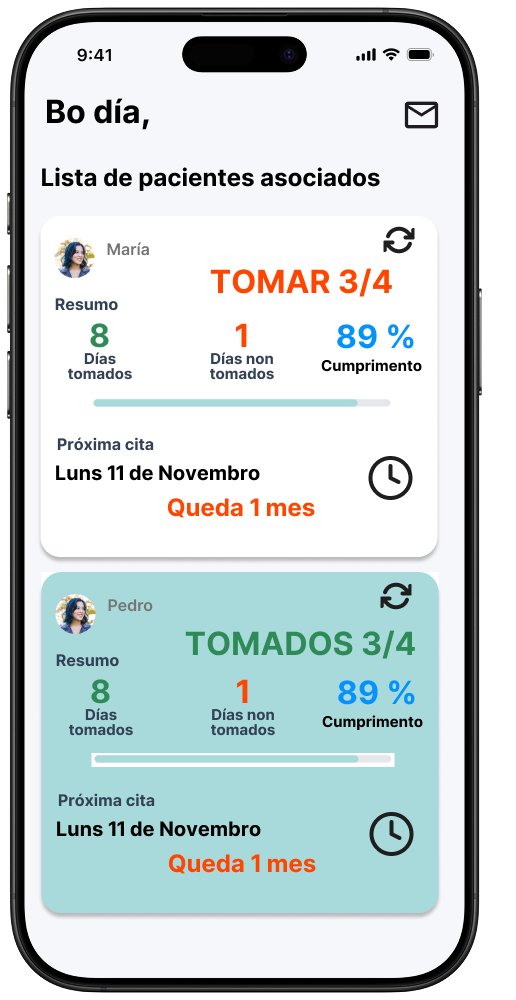
\includegraphics[width=\linewidth]
        {imaxes/07-Deseño/anexo/wireframes/Inicio supervisor toma realizada e varios apcientes.png}
        \caption{Supervisor con varios pacientes.}
        \label{fig:wireframe-inicio-supervisor-varios-pacientes}
    \end{subfigure}
    \hfill
    \begin{subfigure}[t]{0.26\textwidth}
        \centering
        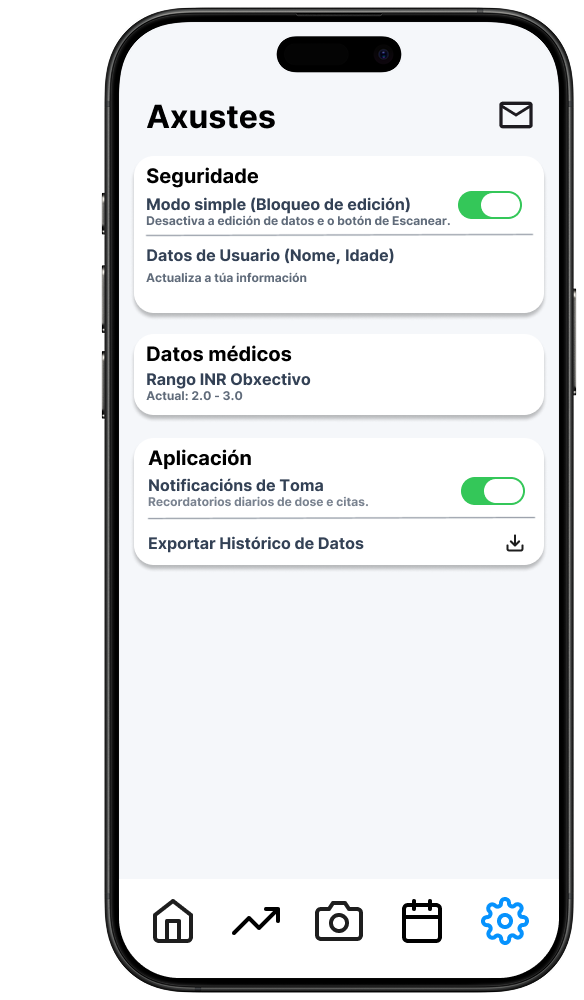
\includegraphics[width=\linewidth]
        {imaxes/07-Deseño/anexo/wireframes/Axustes.png}
        \caption{Axustes da aplicación.}
        \label{fig:wireframe-axustes}
    \end{subfigure}

    \caption{Wireframes do perfil supervisor, da vinculación e dos axustes da aplicación.}
    \label{fig:wireframes-supervisor}
\end{figure}

\begin{figure}[htbp]
    \centering

    \begin{subfigure}[t]{0.23\textwidth}
        \centering
        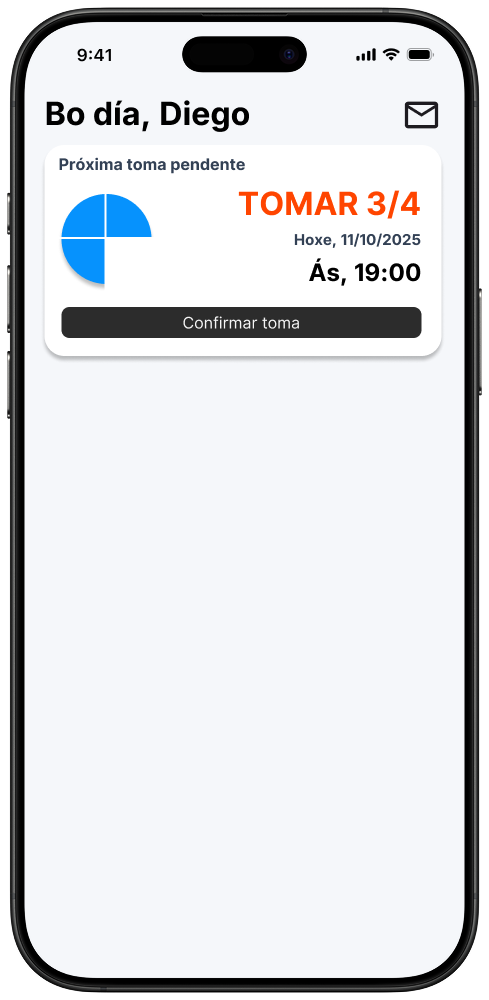
\includegraphics[width=\linewidth]{imaxes/07-Deseño/anexo/wireframes/mock_sinxelo.png}
        \caption{Pantalla principal no modo sinxelo.}
    \end{subfigure}
    \hspace{0.04\textwidth}
    \begin{subfigure}[t]{0.23\textwidth}
        \centering
        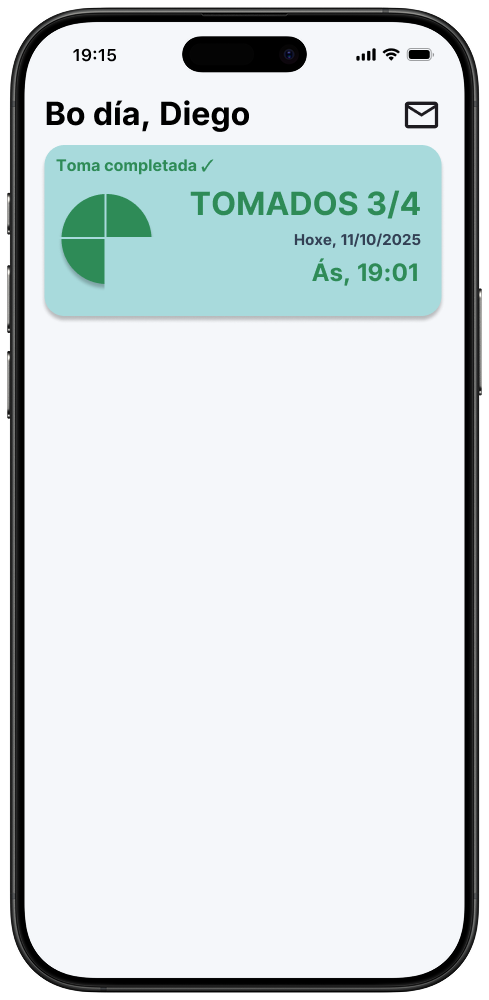
\includegraphics[width=\linewidth]{imaxes/07-Deseño/anexo/wireframes/mock_sinxelo2.png}
        \caption{Acceso aos axustes no modo sinxelo.}
    \end{subfigure}

    \caption{Wireframes correspondentes ao modo sinxelo da aplicación.}
    \label{fig:wireframes-modo-sinxelo-anexo}
\end{figure}
%\include{anexos/...}

 \printglossary[type=\acronymtype,title=\nomeglosarioacronimos]
 \printglossary[title=\nomeglosariotermos]

 \bibliographystyle{IEEEtranN}
 \bibliography{\bibconfig,bibliografia/bibliografia}
 \clearpage
 
\end{document}

%%%%%%%%%%%%%%%%%%%%%%%%%%%%%%%%%%%%%%%%%%%%%%%%%%%%%%%%%%%%%%%%%%%%%%%%%%%%%%%%
